%%%%%%%%%%%%%%%%%%%%%%%%%%%%%%%%%%%%%%%%%
% KOMA-Script Presentation
% LaTeX Template
% Version 1.1 (18/10/15)
%
% This template has been downloaded from:
% http://www.LaTeXTemplates.com
%
% Original Authors:
% Marius Hofert (marius.hofert@math.ethz.ch)
% Markus Kohm (komascript@gmx.info)
% Described in the PracTeX Journal, 2010, No. 2
%
% License:
% CC BY-NC-SA 3.0 (http://creativecommons.org/licenses/by-nc-sa/3.0/)
%
%%%%%%%%%%%%%%%%%%%%%%%%%%%%%%%%%%%%%%%%%

%----------------------------------------------------------------------------------------
%	PACKAGES AND OTHER DOCUMENT CONFIGURATIONS
%----------------------------------------------------------------------------------------
% KOMA-Script_MDPI_jpm-1309345
% compiling only on TexLive 2019

\documentclass[
paper=landscape,
paper=160mm:90mm, %128mm:96mm, % The same paper size as used in the beamer class
fontsize=11pt, % Font size
pagesize, % Write page size to dvi or pdf
parskip=half-, % Paragraphs separated by half a line
%captions=tableheading
]{scrartcl} % KOMA script (article)

\linespread{1.12} % Increase line spacing for readability



%~~~~~~~~~~~~~~~~~~~~~~~~~~~~~~~~~~~~~~~~~~~~~~~
% from main.tex
%%%%%%%%%%%%%%%%%%%%%%%%%%%%%%%%%% Tex
\maxdeadcycles=1000 % Output loop---200 consecutive dead cycles.

% http://mirror.ox.ac.uk/sites/ctan.org/macros/latex/contrib/biblatex/doc/biblatex.pdf it is compatible with KOMA-script
%\usepackage[backend=biber, style=authoryear, sorting=nyt, natbib=false]{biblatex}
% ****** backend=bibtex *******
\usepackage[backend=bibtex, style=authoryear]{biblatex}
%\bibliography{TCGA_margin_cutoff.bib, betel.bib, TMSB4X.bib, pvalueTex.bib}
% ~\autocite{}
\addbibresource{TCGA_margin_cutoff}
\addbibresource{betel.bib}
\addbibresource{TMSB4X.bib}
\addbibresource{pvalueTex.bib}
\addbibresource{Deep_Learning.bib}
% for citep
%\usepackage[comma,authoryear,square]{natbib} 
%\setcitestyle{authoryear,open={[},close={]}}
%\PassOptionsToPackage{comma,authoryear,square}{natbib}

\usepackage{wrapfig} % for wrapfigure, text wrapping figure

\usepackage{todonotes}

\usepackage{floatrow} % for side caption (beside)
%\floatsetup[widefigure]{margins=hangleft,capposition=beside,capbesideposition={center,outside},floatwidth=\textwidth} % {center,outside}
\usepackage{amsmath,amsfonts}
\usepackage{tikz-imagelabels} % for  tikz
%\usepackage[]{caption} % bf
%\newcommand{\bcaption}[2]{\caption{\textbf{#1} #2}}
%\usepackage{outlines}
% mark in blue or red
%\usepackage{xcolor}

%\usepackage{xr-hyper}
\usepackage{hyperref} % for \url clickable
%\newcommand{\R}[1]{\label{#1}\linelabel{#1}} % for \label page and line
%\newcommand{\R}[1]{\linelabel{#1}} % for \label page and line
%\newcommand{\lr}[1]{page~\pageref{#1} (line~\lineref{#1})} % for \ref page and line
% for xr in your preamble
% https://www.overleaf.com/learn/how-to/Cross_referencing_with_the_xr_package_in_Overleaf
%\makeatletter
%\newcommand*{\addFileDependency}[1]{% argument=file name and extension
%  \typeout{(#1)}
%  \@addtofilelist{#1}
%  \IfFileExists{#1}{}{\typeout{No file #1.}}
%}
%\makeatother

%\newcommand*{\myexternaldocument}[1]{%
%    \externaldocument{#1}%
%    \addFileDependency{#1.tex}%
%    \addFileDependency{#1.aux}%
%}
% my external document I would like to reference the labels of. 
%\myexternaldocument{Supplementary_figures} %.tex .aux


%% not tikz
%\usepackage{pstricks-add}
%\usepackage{pst-all} % for PSTricks
%\usepackage{pst-plot,pst-eucl}
%\psset{algebraic,saveNodeCoors}

%\def\f{x+.5}
%\def\g{y-.5}% inverse of \f
%https://tex.stackexchange.com/questions/120788/draw-line-from-a-point-to-another-line-along-x-axis-or-y-axis-in-tikz/120817
%%
\usepackage{array}
\usepackage{ragged2e}
\usepackage{rotating}
\usepackage{tabularx} % for resizebox?
\usepackage{makecell}
% \usepackage{array}
\usepackage{multirow}
\usepackage{colortbl}     % arrayrulecolor
% \usepackage{colortbl}
\usepackage{longtable}

\usepackage{hhline}
%\usepackage{soul} % for \hl{}
\usepackage{siunitx} % for  1e-10 scientific notation, \num
%\usepackage{caption}
%\usepackage{subcaption}
%\usepackage{subcaption} % for figure  side by side, subfigure

%DIF 140a141
\usepackage{pbox} %DIF > 
%DIF -------

\usepackage{booktabs, multirow} % for borders and merged ranges
\usepackage{soul}% for underlines
%\usepackage[table]{xcolor} % for cell colors
\usepackage{changepage,threeparttable} 

%%% for abbreviations, or acronyms
\usepackage[acronym, nopostdot]{glossaries}  % automake
\usepackage{glossary-inline}
%\setacronymstyle{long-short}
%\renewcommand*{\glossarysection}[2][]{} 
%\renewcommand*{\glossarysection}[2][]{\textbf{#1}: }
% for abbreviations environment
%\newcommand{\abbrlabel}[1]{\makebox[3cm][l]{\textbf{#1}\ \dotfill}}
\newenvironment{abbreviation}


%\section{abbreviation}
%%%%%%%%%%%%% Define abbreviation
%\makeglossaries %https://tex.stackexchange.com/questions/110095/list-of-acronyms-is-not-displayed

\newacronym{tmuh}{TMUH}{Taipei Medical University Hospital}

\newacronym{ptta}{PTTA}{p value of t-test or ANOVA}
\newacronym{anova}{ANOVA}{analysis of variance}
\newacronym{lcms}{LC-MS/MS}{liquid chromatography with tandem mass spectrometry}
\newacronym{maldi}{MALDI MS}{matrix-assisted laser desorption/ionization mass spectrometry}
\newacronym{maldii}{MALDI IMS}{matrix-assisted laser desorption/ionization imaging mass spectrometry}


\newacronym{ncbi}{NCBI}{National Center for Biotechnology Information}
\newacronym{degs}{DEGs}{differentially expressed genes}

\newacronym{ihc}{IHC}{immunohistochemistry}
\newacronym{fdr}{FDR}{false discovery rate}

\newacronym{hpa}{HPA}{the Human Protein Atlas}
\newacronym{hnscc}{HNSCC}{head and neck squamous cell carcinoma}
\newacronym{tcga}{TCGA}{the Cancer Genome Atlas}
\newacronym{tcpa}{TCPA}{the Cancer Proteome Atlas}
\newacronym{rna}{RNA}{ribonucleic acid}
\newacronym{rnaseq}{RNA-Seq}{RNA sequencing}
\newacronym{lncrna}{lncRNA}{long non-coding RNA}
%\newacronym{km}{KM}{Kaplan--Meier}
\newacronym{rppa}{RPPAs}{reverse-phase protein arrays}
\newacronym{rpma}{RPMA}{reverse-phase protein lysate microarray}

\newacronym{mmp}{MMP}{matrix metalloproteinase}
 %DKK1, CAMK2N1, STC2, PGK1, SURF4, USP10, NDFIP1, FOXA2, STIP1, and DKC1
 %ZNF557, ZNF266, IL19, MYO1H, FCGBP, LOC148709, EVPLL, PNMA5, KIAA1683, and NPB

\newacronym{DKK1}{DKK1}{dickkopf WNT signaling pathway inhibitor 1} 
\newacronym{CAMK2N1}{CAMK2N1}{calcium/calmodulin dependent protein kinase II inhibitor 1} 
\newacronym{CALML5}{CALML5}{calmodulin like 5}

\newacronym{STC2}{STC2}{stanniocalcin 2} 
\newacronym{PGK1}{PGK1}{phosphoglycerate kinase 1} 
\newacronym{SURF4}{SURF4}{surfeit 4} 
\newacronym{USP10}{USP10}{ubiquitin specific peptidase 10} 
\newacronym{NEDD4}{NEDD4}{neural precursor cell expressed, developmentally down-regulated 4}
\newacronym{NDFIP1}{NDFIP1}{NEDD4 family interacting protein 1} 
\newacronym{FOXA2}{FOXA2}{forkhead box A2} 
\newacronym{STIP1}{STIP1}{stress-induced-phosphoprotein 1} 
\newacronym{DKC1}{DKC1}{dyskeratosis congenita 1, dyskerin} 

\newacronym{ZNF557}{ZNF557}{zinc finger protein 557} 
\newacronym{ZNF266}{ZNF266}{zinc finger protein 266} 
\newacronym{IL19}{IL19}{interleukin 19} 
\newacronym{MYO1H}{MYO1H}{myosin 1H} 
\newacronym{FCGBP}{FCGBP}{Fc fragment of IgG binding protein} 
\newacronym{LOC148709}{LOC148709}{LncRNA LOC148709} 
\newacronym{EVPLL}{EVPLL}{envoplakin-like protein} 
\newacronym{PNMA5}{PNMA5}{paraneoplastic antigen like 5} 
%\newacronym{KIAA1683}{KIAA1683}{IQCN, IQ Motif Containing N} 
\newacronym{IQCN}{IQCN}{IQ motif containing N} % previous name KIAA1683
% "IQ'' refers to the first two amino acids of the motif: isoleucine (commonly) and glutamine (invariably)
\newacronym{NPB}{NPB}{neuropeptide B} 

 \newacronym{rt}{RT}{radiation therapy}
 \newacronym{nccn}{NCCN}{National Comprehensive Cancer Network}
 \newacronym{hif}{HIF}{hypoxia-inducible factor}
 \newacronym{egfr}{EGFR}{epidermal growth factor receptor}
 \newacronym{ras}{RAS}{rat sarcoma}
 \newacronym{hras}{HRAS}{Harvey rat sarcoma viral oncoprotein}
 \newacronym{erk}{ERK}{extracellular signal-regulated kinases}
 \newacronym{us}{US}{United States}
 \newacronym{fda}{FDA}{Food and Drug Administration}
 \newacronym{tpf}{Tax-PF}{docetaxel, cisplatin, and 5-fluorouracil}
 \newacronym{tki}{TKI}{tyrosine kinase inhibitor}
 \newacronym{her}{HER}{human epidermal growth factor receptor}
 \newacronym{ici}{ICI}{immune-checkpoint inhibitor}
 \newacronym{ctla4}{CTLA-4}{cytotoxic T lymphocyte antigen 4}
 \newacronym{pd1}{PD-1}{programmed death 1}
 \newacronym{pdl1}{PD-L1}{programmed death ligand 1}
 \newacronym{tim3}{TIM-3}{T-cell immunoglobulin mucin protein 3}
 \newacronym{lag3}{LAG-3}{lymphocyte activation gene 3}
 \newacronym{ifng}{IFN-$\gamma$}{interferon gamma}
 \newacronym{tigit}{TIGIT}{T cell immunoglobin and immunoreceptor tyrosine-based inhibitory motif}
 \newacronym{gitr}{GITR}{glucocorticoid-induced tumor necrosis factor receptor}
 \newacronym{vista}{VISTA}{V-domain Ig suppressor of T-cell activation}
 \newacronym{tmsb4x}{TMSB4X}{thymosin beta-4 X-linked}
 \newacronym{emt}{EMT}{epithelial-mesenchymal-transition}
 \newacronym{gdc}{GDC}{Genomic Data Commons}
 \newacronym{nci}{NCI}{the National Cancer Institute}
 \newacronym{gdac}{GDAC}{genome data analysis center}
 \newacronym{rest}{REST}{Representational State Transfer} 
 \newacronym{api}{API}{application programmable interface}
\newacronym{grch38}{GRCh38}{Genome Reference Consortium Homo sapiens genome assembly 38}
\newacronym{fpkm}{FPKM}{Fragments per kilobase per million reads mapped}
\newacronym{rsem}{RSEM}{RNA-Seq by Expectation-Maximization}
\newacronym{slca}{SLC35E2A}{solute carrier family 35 member E2A}
\newacronym{slcb}{SLC35E2B}{solute carrier family 35 member E2B}
\newacronym{cde}{CDE}{Common Data Element}
\newacronym{id}{ID}{identification}
\newacronym{ajcc}{AJCC}{the American Joint Committee on Cancer}
\newacronym{uicc}{UICC}{he Union for International Cancer Control}
\newacronym{tnm}{TNM}{the tumor size (T), cervical lymph node metastases (N), and distal metastasis status (M)}
\newacronym{ci95}{95\% CI}{95\% confidence interval}
\newacronym{os}{OS}{overall survival}
\newacronym{hr}{HR}{hazard ratio}
\newacronym{hpv}{HPV}{human papillomavirus}
\newacronym{ene}{ENE}{extra-nodal extension}
\newacronym{lvsi}{LVSI}{lymph-vascular space invasion}
\newacronym{pni}{PNI}{perineural invasion}
\newacronym{doi}{DOI}{depth of invasion}
\newacronym{lnd}{LND}{lymph node density}
\newacronym{wpoi5}{WPOI-5}{worst pattern of invasion score 5}
\newacronym{glut4}{GLUT4}{glucose transporter 4}
\newacronym{slc2a4}{SLC2A4}{solute carrier family 2 member A4}
\newacronym{trim24}{TRIM24}{tripartite motif-containing 24}
\newacronym{til}{TIL}{tumor-infiltrating lymphocytes}
\newacronym{tmb}{TMB}{tumor mutational burden}




%------------------------------------------------
\usepackage{outlines}
\usepackage[font={small}]{caption}
\newcommand{\bcaption}[2]{\caption{\textbf{#1} #2}}


\usepackage[margincaption]{sidecap}

\usepackage{subcaption} % for figure  side by side, subfigure

%%%%%% updated 2020 by esdd
%% https://tex.stackexchange.com/questions/547723/latex-throws-errors-on-section
%------------------------------------------------
% Colors
\usepackage[]{xcolor}  % table % Required for custom colors
% Define a few colors for making text stand out within the presentation
\definecolor{mygreen}{RGB}{44,85,17}
\definecolor{myblue}{RGB}{34,31,217}
\definecolor{mybrown}{RGB}{194,164,113}
\definecolor{myred}{RGB}{255,66,56}
% Use these colors within the presentation by enclosing text in the commands below

\newcommand*{\mygreen}[1]{\textcolor{mygreen}{#1}}
\newcommand*{\myblue}[1]{\textcolor{myblue}{#1}}
\newcommand*{\mybrown}[1]{\textcolor{mybrown}{#1}}
\newcommand*{\myred}[1]{\textcolor{myred}{#1}}

\definecolor{asparagus}{rgb}{0.53, 0.66, 0.42}

\newenvironment{MyColorPar}[1]{% for RED marked of revision
    \leavevmode\color{#1}\ignorespaces%
}{%
}%


% Margins
\usepackage[ % Page margins settings
  includeheadfoot,
  top=-1mm,
  bottom=1.5mm,
  left=1mm,
  right=3.5mm,
  headsep=0mm,
  footskip=8.5mm
]{geometry}

% Fonts
\usepackage[T1]{fontenc}     % For correct hyphenation and T1 encoding
\usepackage{lmodern} % Default font: latin modern font
%\usepackage{fourier} % Alternative font: utopia
%\usepackage{charter} % Alternative font: low-resolution roman font
\renewcommand{\familydefault}{\sfdefault} % Sans serif - this may need to be commented to see the alternative fonts

% Various required packages
\usepackage{amsthm} % Required for theorem environments
\usepackage{bm} % Required for bold math symbols (used in the footer of the slides)
\usepackage{tikz} % Required for colored boxes, loads graphicx and other packages
\usepackage{booktabs} % Required for horizontal rules in tables
\usepackage{multicol} % Required for creating multiple columns in slides
\usepackage{lastpage} % For printing the total number of pages at the bottom of each slide

\usepackage{microtype} % Better typography

% Slide layout configuration
\usepackage[automark]{scrlayer-scrpage} % Required for customization of the header and footer
\clearpairofpagestyles % Remove the default header and footer
\AddLayersAtBeginOfPageStyle{scrheadings}{headerbg,footerbg}% add background layers
\setkomafont{pageheadfoot}{\normalfont\sffamily} % Font settings for the header and footer
\setkomafont{pagehead}{\color{white}}
% Header configuration - if you don't want a header remove this block
\DeclareNewLayer[
  background,
  head,
  hoffset=0pt,
  width=\paperwidth,
  mode=picture,
  contents=\putLL{\myblue{\rule{\layerwidth}{\layerheight}}}
]{headerbg}

\ihead{\rightbotmark}

% Footer configuration
\KOMAoptions{footwidth=\textwidth+2mm:0pt}
\setkomafont{pagefoot}{\color{black}\tiny} % Small font size for the footnote
%\DeclareNewLayer[
  %background,
  %foot,
  %hoffset=0pt,
  %width=\paperwidth,
  %mode=picture,
  %contents=\putLL{\myblue{\rule{\layerwidth}{\layerheight}}}
%]{footerbg}
\ifoot{\myauthor\ \raisebox{0.2mm}{$\bm{\vert}$}\ \myuni} % Left side text
\ofoot*{\pagemark/\pageref{LastPage}} % Right side

% Sets vertical centering of slide contents with increased space between paragraphs/lists
\makeatletter
\renewcommand*{\@textbottom}{\vskip \z@ \@plus 1fil}
\newcommand*{\@texttop}{\vskip \z@ \@plus .5fil}
\setparsizes{1em}{\z@\@plus .25fil}{0pt plus 1fil}
\makeatother

% Remove page numbers and the dots leading to them from the outline slide
\DeclareTOCStyleEntries[linefill=\hfill,pagenumberbox=\gobble]{section}{section,subsection,subsubsection}
%\newcommand*\gobble[1]{}
\AfterTOCHead{\small}

%\renewcaptionname{english}{\contentsname}{Outline} % contentsname % Change the name of the table of contents
% Section spacing - deeper section titles are given less space due to lesser importance
\RedeclareSectionCommands[beforeskip=0pt,afterskip=0pt,afterindent=true,runin=false]{section,subsection,subsubsection}
\RedeclareSectionCommand[afterskip=-1mm]{subsection}
\RedeclareSectionCommand[afterskip=-2mm]{subsubsection}
\setcounter{secnumdepth}{\partnumdepth} % How deep sections are numbered

% Theorem style
\newtheoremstyle{mythmstyle} % Defines a new theorem style used in this template
  {0.5em} % Space above
  {0.5em} % Space below
  {} % Body font
  {} % Indent amount
  {\sffamily\bfseries} % Head font
  {} % Punctuation after head
  {\newline} % Space after head
  {\thmname{#1}\ \thmnote{(#3)}} % Head spec

\theoremstyle{mythmstyle} % Change the default style of the theorem to the one defined above
\newtheorem{theorem}{Theorem}[section] % Label for theorems
\newtheorem{remark}[theorem]{Remark} % Label for remarks
\newtheorem{algorithm}[theorem]{Algorithm} % Label for algorithms


% The code for the box which can be used to highlight an element of a slide (such as a theorem)
\newcommand*{\mybox}[2]{% The box takes two arguments: width and content
  \par\noindent
  \begin{tikzpicture}[mynodestyle/.style={rectangle,draw=myblue,thick,inner sep=2mm,text justified,top color=white,bottom color=white,above}]
    \node[mynodestyle,at={(0.5*#1+2mm+0.4pt,0)}]{% Box formatting
      \begin{minipage}[t]{#1}
      #2
      \end{minipage}%
    };
  \end{tikzpicture}
\par\vspace{-1.3em}}

%----------------------------------------------------------------------------------------
%	PRESENTER INFORMATION Tex Chi
%----------------------------------------------------------------------------------------
\usepackage{mfirstuc}
\MFUnocap{and}
\MFUnocap{for}
\MFUnocap{in}
% dissertation title: \title{\capitalisewords{global transcriptomics and proteomics analyses for biomarker identification and validation in head and neck squamous cell carcinoma}}
\newcommand*{\mytitle}{\capitalisewords{A Transcriptomic Analysis of Head and Neck Squamous Cell Carcinomas for Prognostic Indications}}
%global transcriptomics and proteomics analyses for biomarker identification and validation in head and neck squamous cell carcinoma}}
%\newcommand*{\mytitle}{Global Proteomics-based Identification and Validation of Thymosin Beta-4 X-Linked as a Prognostic Marker for Head and Neck Squamous Cell Carcinoma}
% new title: A Transcriptomic Analysis of Head and Neck Squamous Cell Carcinomas for Prognostic Indications
% old Title Transcriptomic Analysis for Prognostic Value in Head and Neck Squamous Cell Carcinoma
\newcommand*{\runninghead}{HNSCC Biomarker} % Running head displayed on almost all slides
\newcommand*{\myauthor}{Li-Hsing (Tex) Chi} % Presenters name(s)
\newcommand*{\myadvisorM}{Michael Hsiao}
\newcommand*{\myadvisorJ}{Yu-Chuan (Jack) Li}
\newcommand*{\myadvisorA}{Alexander TH Wu}
\newcommand*{\mydate}{2022/04/06}
%{2022/01/12} % \today Presentation date {2021/09/10} or {2021/12/10}
\newcommand*{\myuni}{Taipei Medical University} % University or department

\newcommand{\comm}[1]{} % for comment it out; https://tex.stackexchange.com/questions/17816/commenting-out-large-sections
%----------------------------------------------------------------------------------------

\begin{document}

%----------------------------------------------------------------------------------------
%	TITLE SLIDE
%----------------------------------------------------------------------------------------

% Title slide - you may have to tweak a few of the numbers if you wish to make changes to the layout
\thispagestyle{empty} % No slide header and footer


\includegraphics[width=9.5cm]{TMU_PTM_logo.png}
\begin{tikzpicture}[remember picture,overlay] % Background box
  \node [xshift=\paperwidth/2,yshift=\paperheight/2] at (current page.south west)
    [rectangle,fill,inner sep=0pt,minimum width=\paperwidth,minimum height=\paperheight/1.85,top color=myblue,bottom color=myblue]{}; % Change the height of the box, its colors and position on the page here
\end{tikzpicture}
% Text within the box
\begin{flushright}
%  \vspace{0.45cm}
  \color{white}\sffamily
  {\bfseries\Large\mytitle\par}% Title
  \vspace{0.2cm}
  \normalsize
  \myauthor, D.D.S., Ph.D.  \hspace{20mm} \par % Author name
%  Ph.D. candidate: \myauthor  \hspace{28.7mm} \par % Author name
  Advisors: \myadvisorM \hspace{1mm} \myadvisorJ\par \hspace{1mm} \myadvisorA\par
  \mydate %\par % Date
%  \myuni\par
%  \vfill
\end{flushright}
%Chi, L.-H., Wu, A. T. H., Hsiao, M. \& Li, Y.-C. (Jack). Journal of Personalized Medicine, 11, 782 (2021).
%\autocite{Chi2021}
%  \vspace{0.3cm}

\large \hspace{6cm} $\longrightarrow$ A Holistic Way for Cancer Care

\clearpage

%\begin{figure}
%    \centering
%    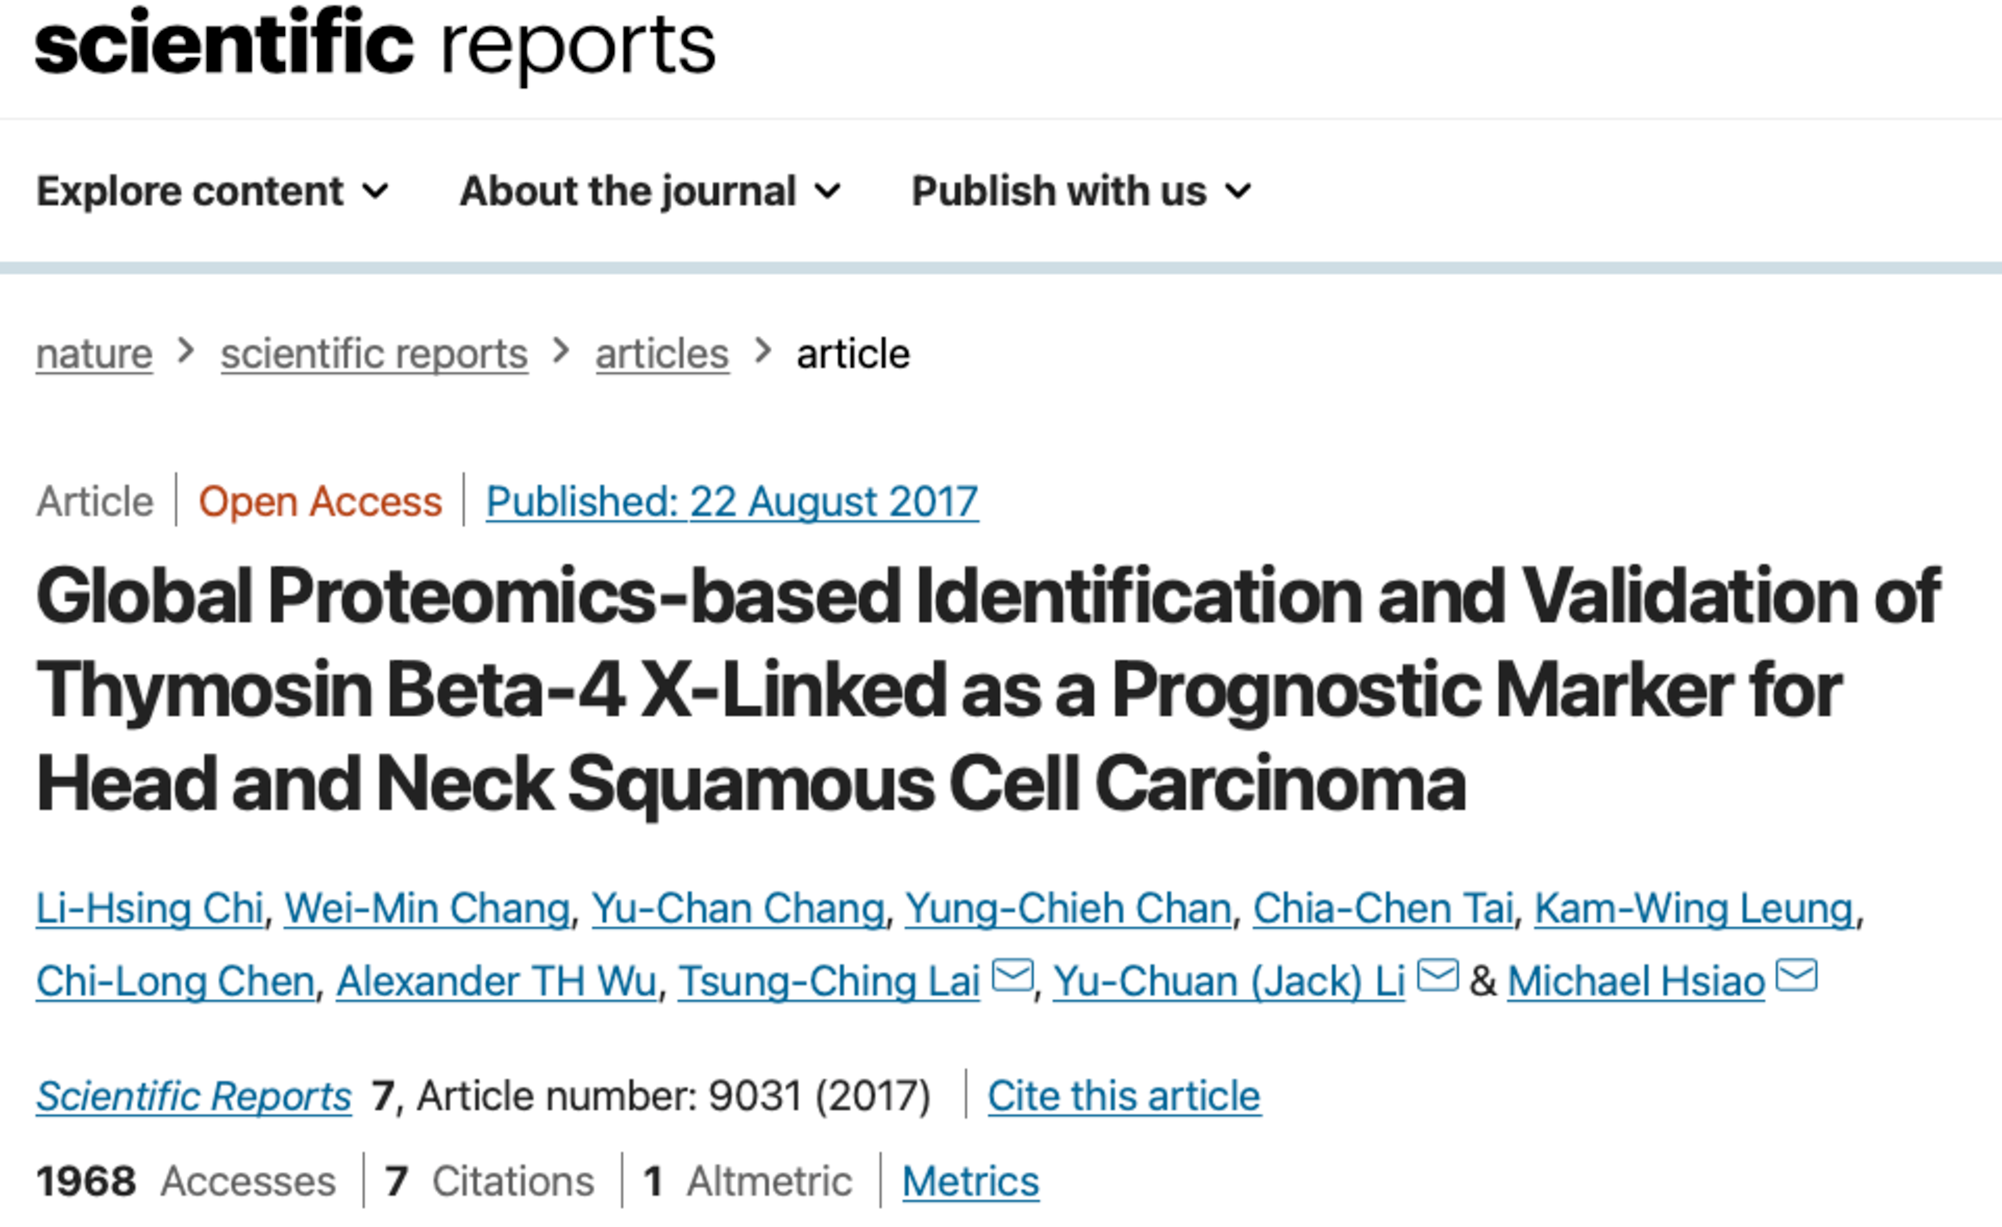
\includegraphics[width=13cm]{Article_Banner_TMSB4X_2017.pdf}
%    \caption{Caption}
%    \label{fig:my_label}
%\end{figure}
%\clearpage
%----------------------------------------------------------------------------------------
%	TABLE OF CONTENTS
%----------------------------------------------------------------------------------------

\thispagestyle{empty} % No slide header and footer

\small\tableofcontents % Change the font size and print the table of contents - it may be useful to shrink the font size further if the presentation is full of sections
% To exclude sections/subsections from the table of contents, put an asterisk after \(sub)section like so: \section*{Section Name}
%\clearpage


\textbf{KEYWORD}\\
%head and neck squamous cell carcinoma (HNSCC);\\
the Cancer Genome Atlas (TCGA); \\
\hl{transcriptomics}; proteomics; \\
\hl{RNA-Seq}: \acrlong{rnaseq};\\ %\hl{mass spectrometry};\\
R; Rstudio server on the cloud; Google platform; firebrowseR;\\
survival analysis; \hl{optimal cutoff} for Kaplan--Meier curve; Cox proportional hazard regression model;\\
\url{https://github.com/texchi2/pvalueTex}; \\
reproducible research; \LaTeX;\\
%effect size; hazard ratio in Cox's modeling;\\
%\acrfull{tmsb4x}; \\
%\acrfull{CALML5}; \\
%\acrfull{FCGBP}; \\
\hl{holistic cancer care}; mindfulness meditation.

\begin{outline}

\1 surgical specimen from oral cancer %口腔癌病理檢體
\2 using Next Generation Sequencing (NGS) to measure the gene expression (\hl{RNA-Seq})

\1 to make a model to estimate biomarkers
\2 association of RNA-Seq versus patient's survival time %基因表現量,與口腔癌症病患存活的相關性

\1 Chi et al, 2021, published at \url{https://www.mdpi.com/2075-4426/11/8/782/htm}
\2 a video abstract available at
\url{https://encyclopedia.pub/16116}

\end{outline}

\clearpage

%----------------------------------------------------------------------------------------
%	PRESENTATION SLIDES
%----------------------------------------------------------------------------------------

%\section*{Vize}

%\clearpage

%------------------------------------------------




\section{Introduction}

\thispagestyle{headings}
\markright{Introduction\hfill Oral cancer is a major disease in Taiwan \hfill}
%\begin{figure}
%\end{figure}



\begin{minipage}[c]{0.60\linewidth}
\begin{outline}
    \1 Head and neck squamous cell carcinoma (HNSCC) in Taiwan, which is:
        \2 derived from the \hl{oral cavity}, oropharynx, hypopharynx and larynx;
        \2 caused by long-term habits of betel nut \hl{[*OR 28.2]}, cigarette [*OR 18.0], alcohol [*OR 10.2]~\autocite{Ko1995}. {\tiny (*odds ratio)}
    \1  HNSCC is a serious problem in Taiwan:
%        \2 The \hl{sixth} common cancer worldwide~\autocite{Siegel2016};
        \2 The age-standardized incidence rate of \acrshort{hnscc} in males is \hl{42.15} per 100,000 person-years~ (7,400 victims/year) ~\autocite{MOHWincidence2018}**;
%        \2 Specialist of otolaryngology, oral and maxillofacial surgery in Taiwan (2021): 2,557 and 431, respectively  
        \2 The \hl{fourth} leading cause of cancer-related death for males in Taiwan (2,779 persons/year)~\autocite{MOHWdeath2017}**.
        {\tiny (**MOHW: Ministry of Health and Welfare, Taiwan)}
\end{outline}
\end{minipage}%\hspace{2mm}
%\begin{wrapfigure}{r}{0.3\textwidth}
\begin{minipage}[c]{0.35\linewidth}
    \raggedright
    \hfill
    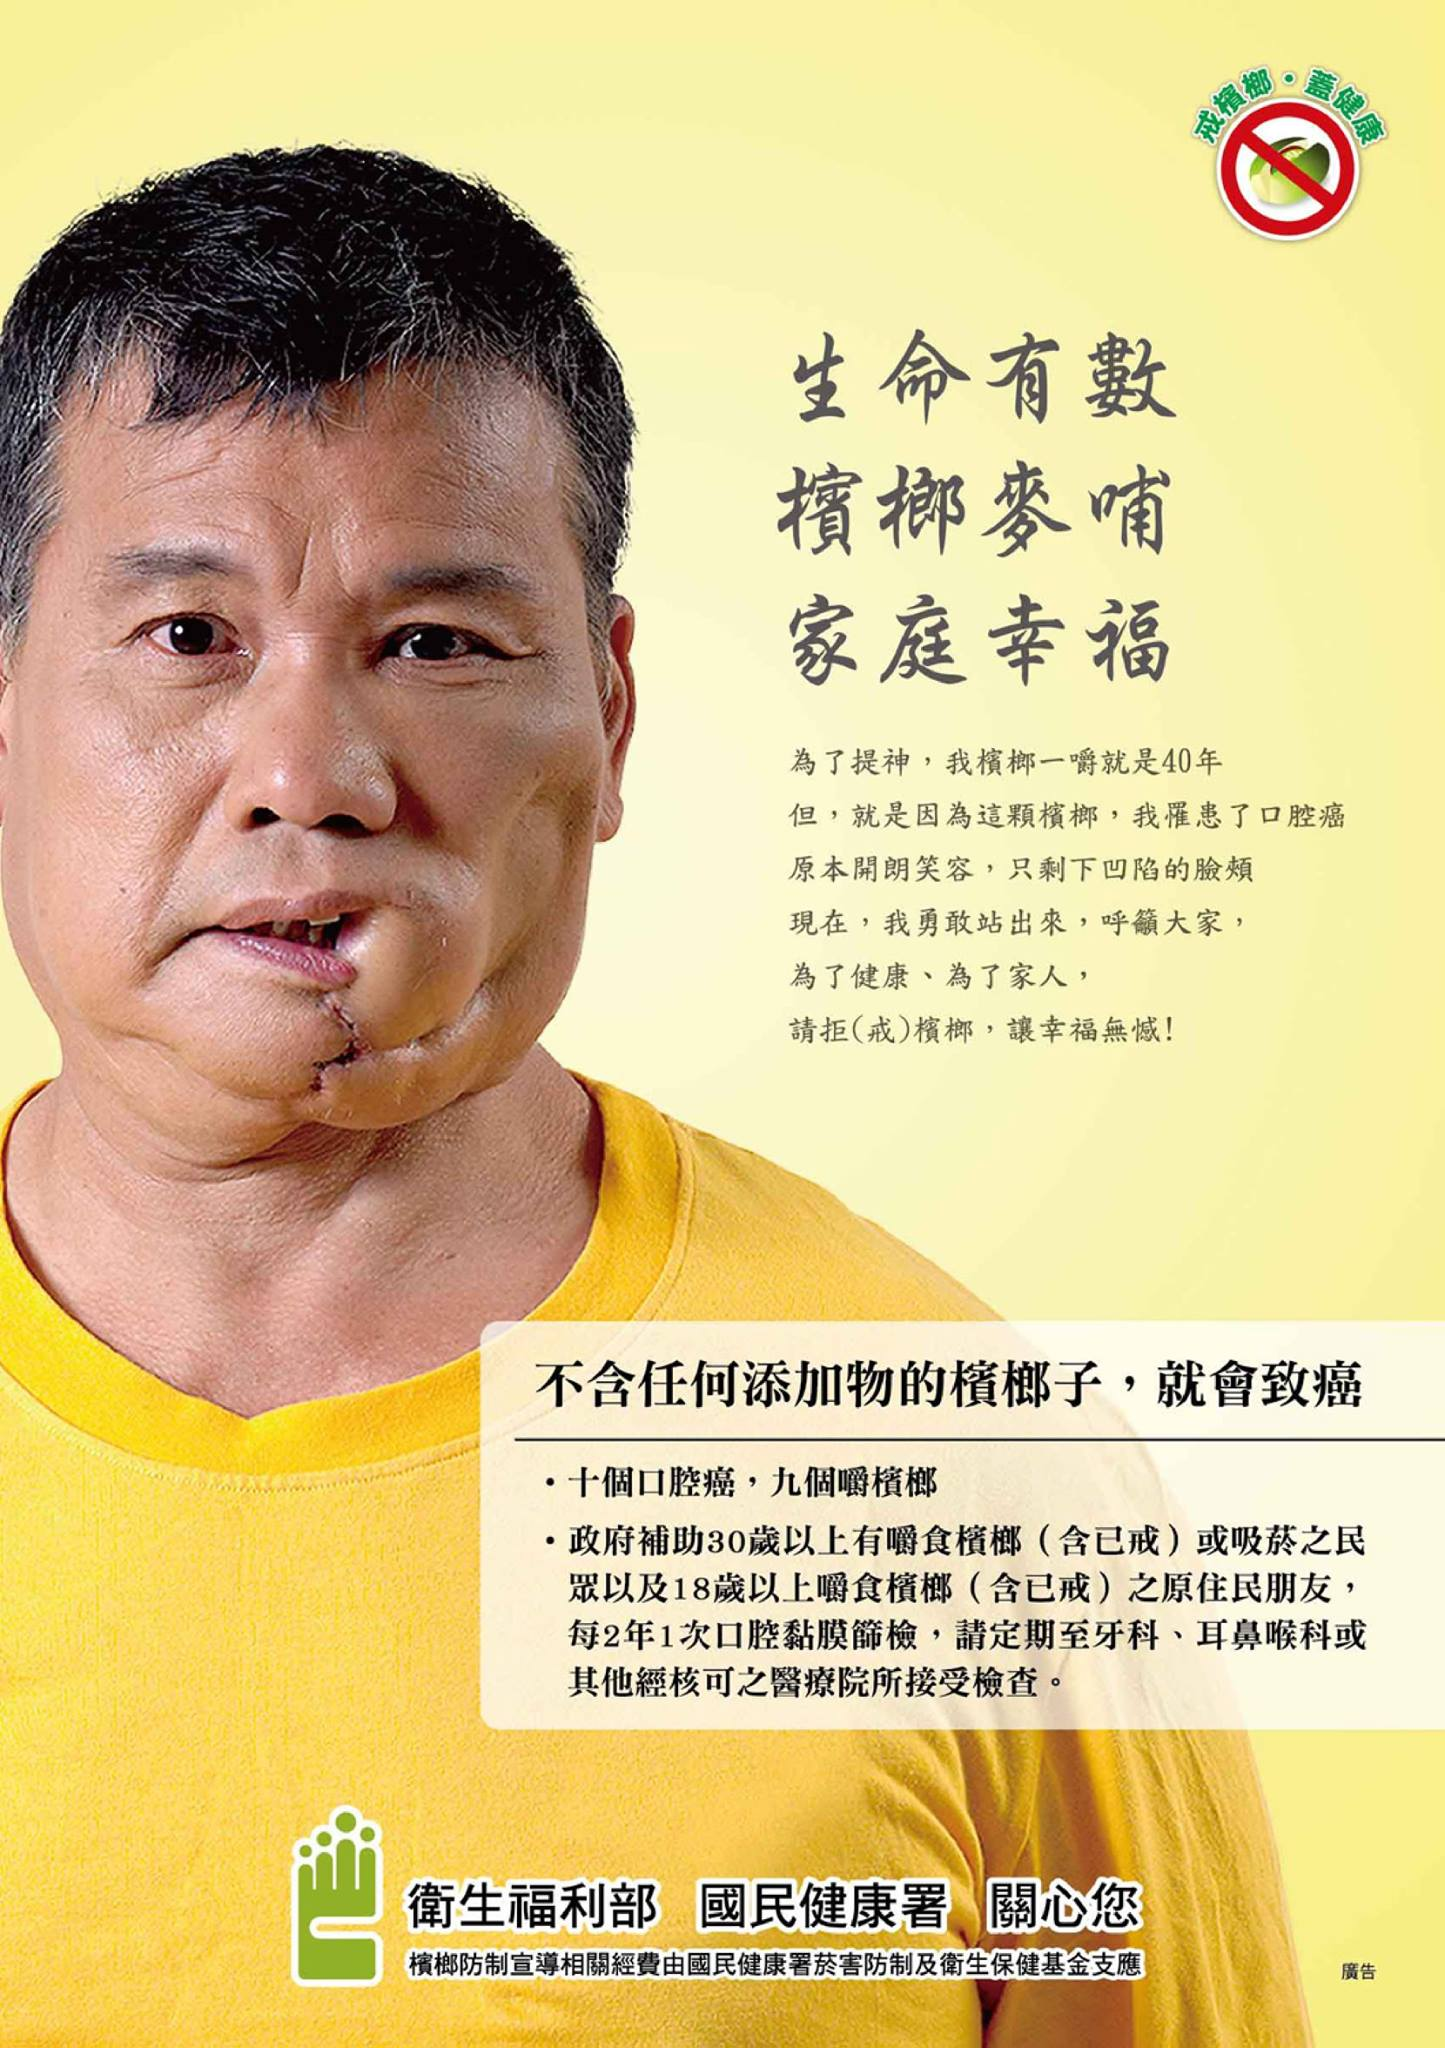
\includegraphics[width=4.5cm]{20369933_1755313531164078_5705495585669958017_o.jpg}\\
    %\caption*{
   \tiny (Photo courtesy of Health Promotion Administration, MOHW, Taiwan.)

\end{minipage}




\clearpage

%%%%%%%%%%%
\thispagestyle{headings}
\markright{Introduction\hfill Biomarker-guided HNSCC therapy \hfill}

%The advantages of applying the TCGA data for cancer biomarker identification include:
\begin{outline}
\1  Treatment for HNSCC: \textcolor{green}{surgery}, radiotherapy, or systemic therapy (chemotherapy/targeted therapy)
%There are many physical and social features of patients available for survival modeling. % ($X_1 ... X_n$)
    \2 \hl{metastasis}: from oral cavity (T*) $\longrightarrow$ neck lymph nodes (N*) $\longrightarrow$ the rest of body (M*) (e.g., lung, liver, bone)
    \2 "Biomarkers" guide the treatment after surgery:
%\1 many achievements and getting published, including \hl{Chi} et al., 2021~\autocite{Chi2021}.
%    \2 diagnostic, \textcolor{red}{predictive} or \textcolor{green}{prognostic} biomarkers:
        \3 pathological marker: \textcolor{red}{\acrfull{doi}} ($> 3 mm$), \textcolor{red}{positive surgical margin} ($< 2 mm$) or \textcolor{red}{positive lymph node (N+)} $\longrightarrow$ adjuvant radiation therapy %\hfill {\tiny (* DOI: \acrlong{doi})} is NOT tumor thickness
        \3 molecular marker: over-expression of \textcolor{red}{EGFR} $\longrightarrow$ targeted inhibitor---cetuximab~\autocite{LeTourneau2007} \hfill {\tiny (covered by Taiwan's National Health Insurance since \hl{2009})}
        % \cite{LeTourneau2007} Leblanc2020
        
        {\tiny (* cancer staging by TNM system: \textcolor{red}{T}umor size/depth, neck \textcolor{red}{N}odal metastasis, distant \textcolor{red}{M}etastasis; \\
        TNM system: the Union for International Cancer Control, UICC, and
        the American Joint Committee on Cancer, AJCC)}
\clearpage

%    \2 "The results published~\autocite{Chi2021} and shown here are in part based upon data generated by the TCGA Research Network: \url{https://www.cancer.gov/tcga}."
\1 50\% recurrent rate (on primary or neck) (all stages, global)~\autocite{Forastiere2001,Warnakulasuriya2009}

\1 However, the \hl{survival} rate in Taiwan (2008 $\longrightarrow$ 2018):
    \2 the one-year survival rate*: 79.56\% $\longrightarrow$ 81.62\% (all stages)
    \2 the five-year survival rate*: 55.13\% $\longrightarrow$ 56.03\% (all stages) \\
    {\tiny * \url{https://cris.hpa.gov.tw/pagepub/Home.aspx}}
\1 We do our best ...
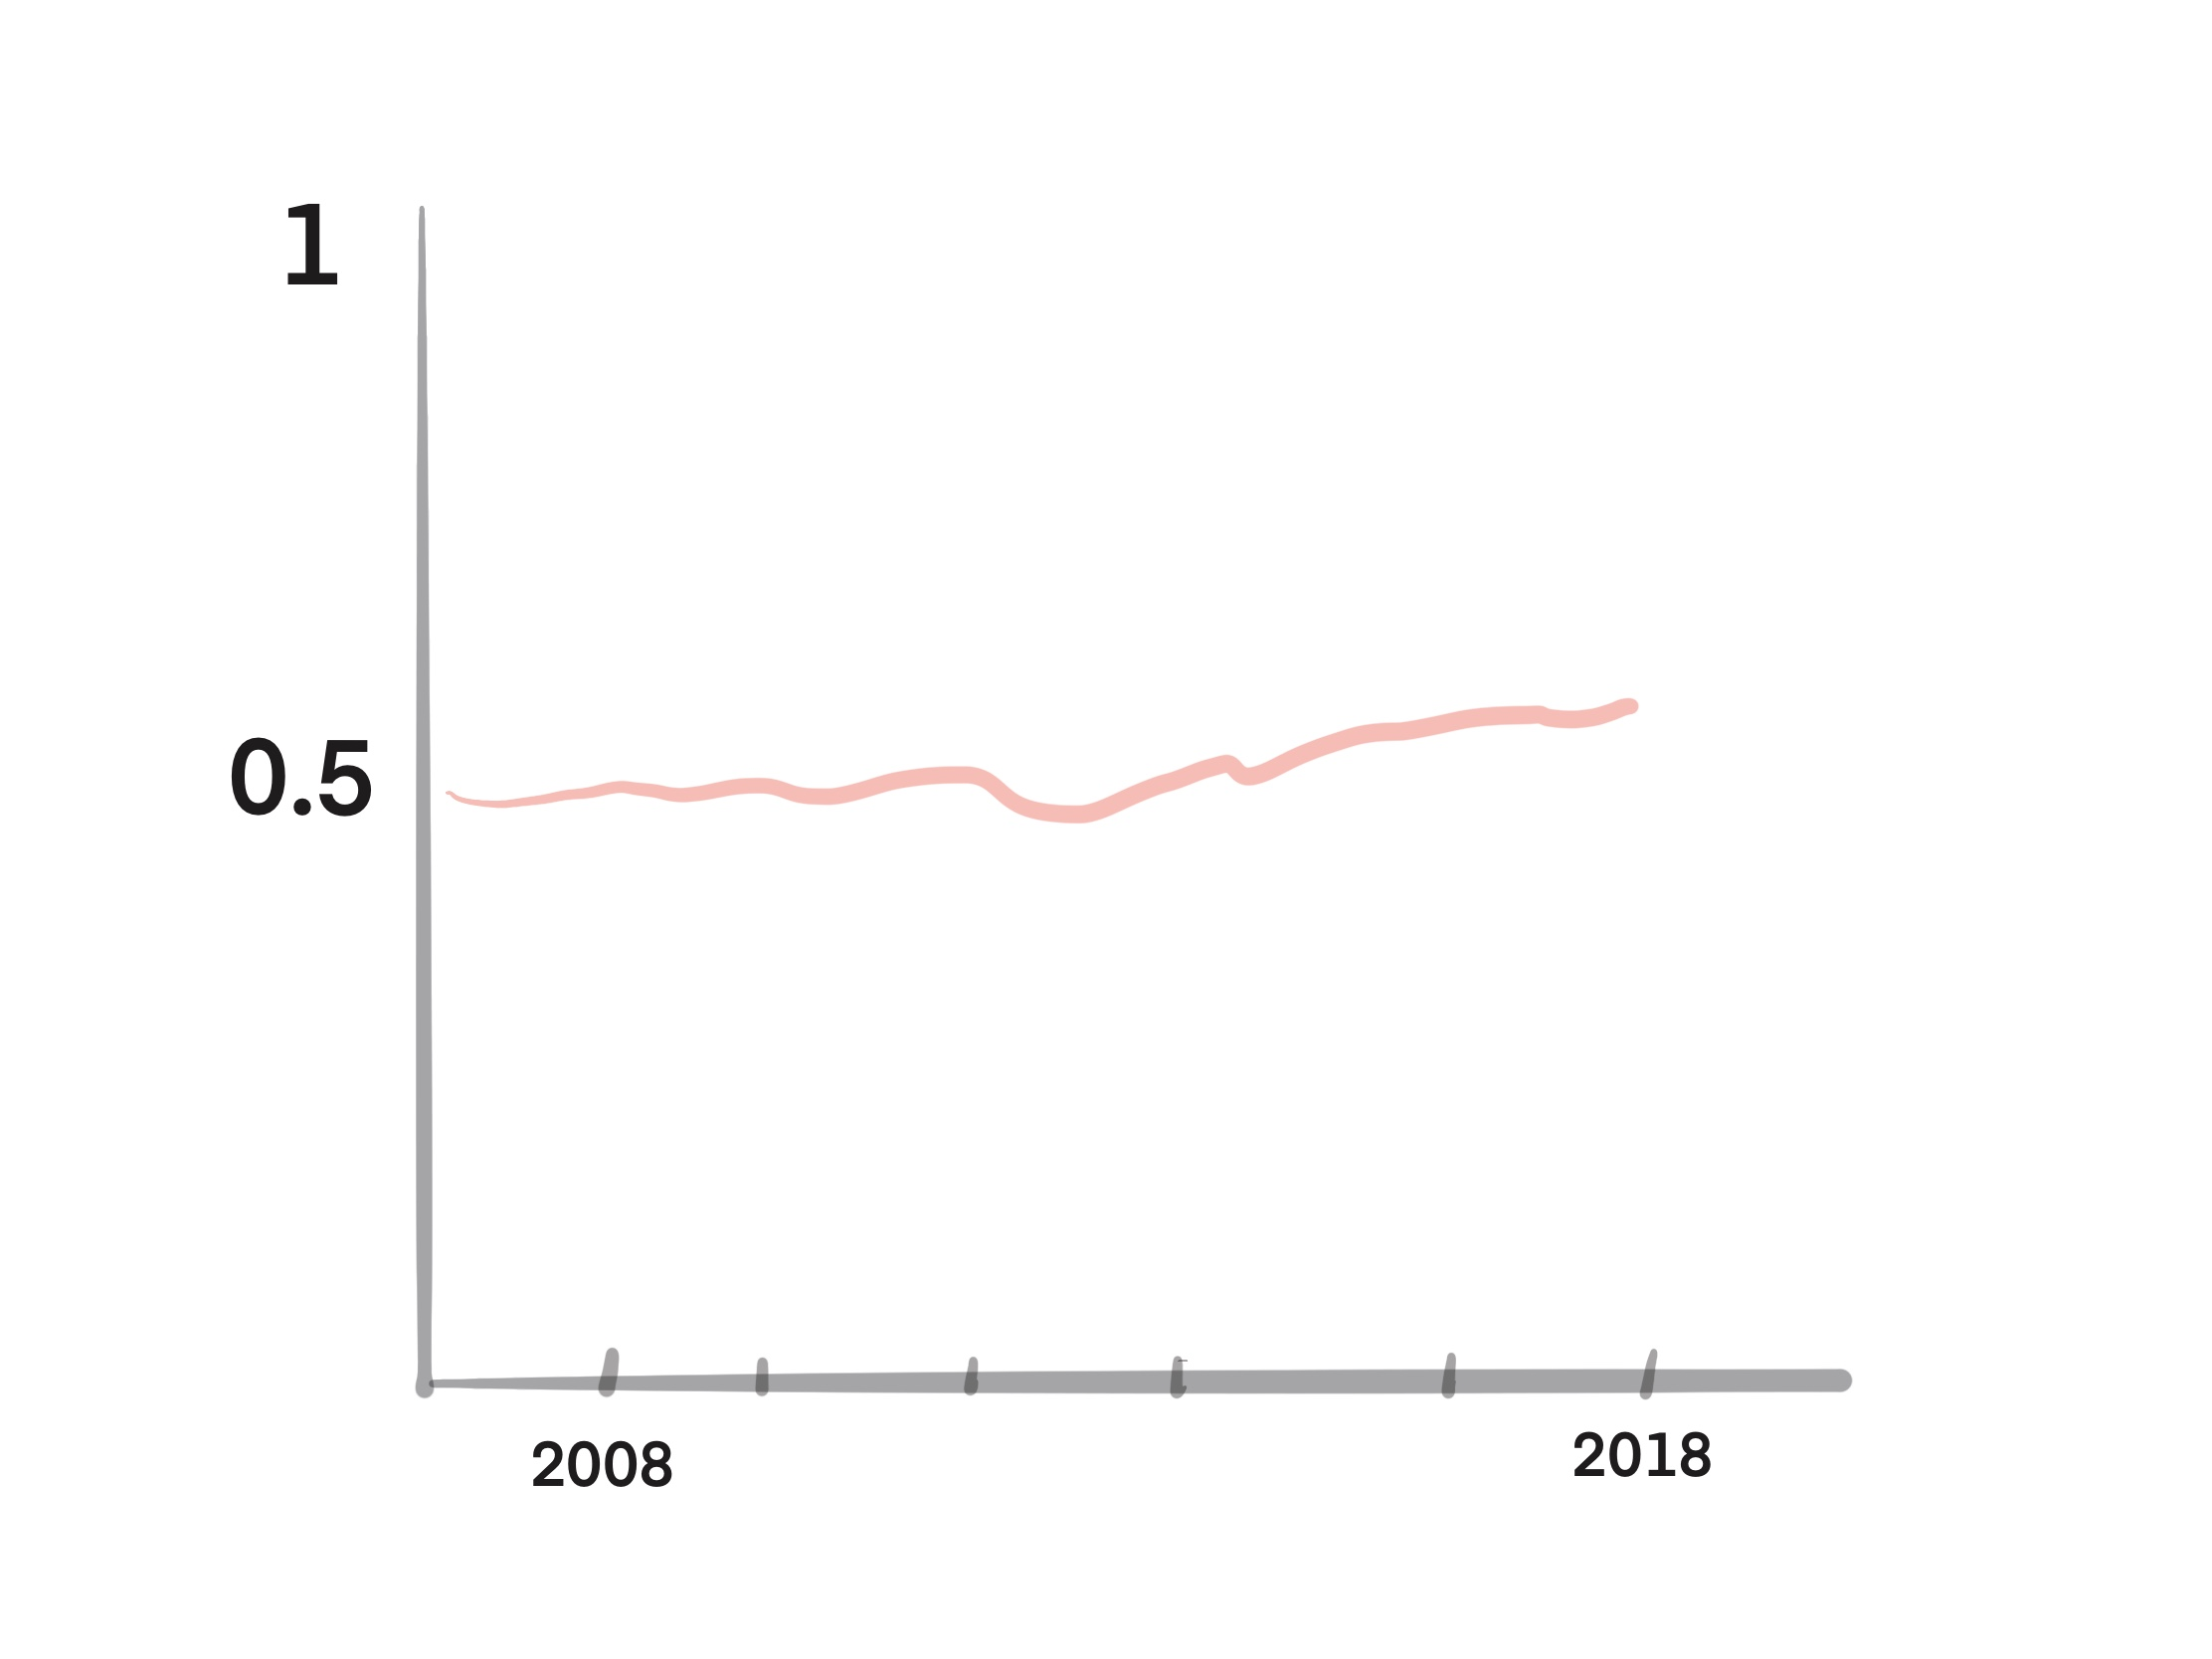
\includegraphics[width=4cm]{stationary_survival_Artwork 2.jpg}


\clearpage


%%
\1 We do
    \2 encourage patients for \hl{correction} of their life style;
    \2 \textcolor{green}{wider excision} (T+N) and better free-flap \textcolor{green}{reconstruction}.
%    \2 to find more useful \textcolor{red}{biomarkers}
\end{outline}
\begin{figure}
    \centering
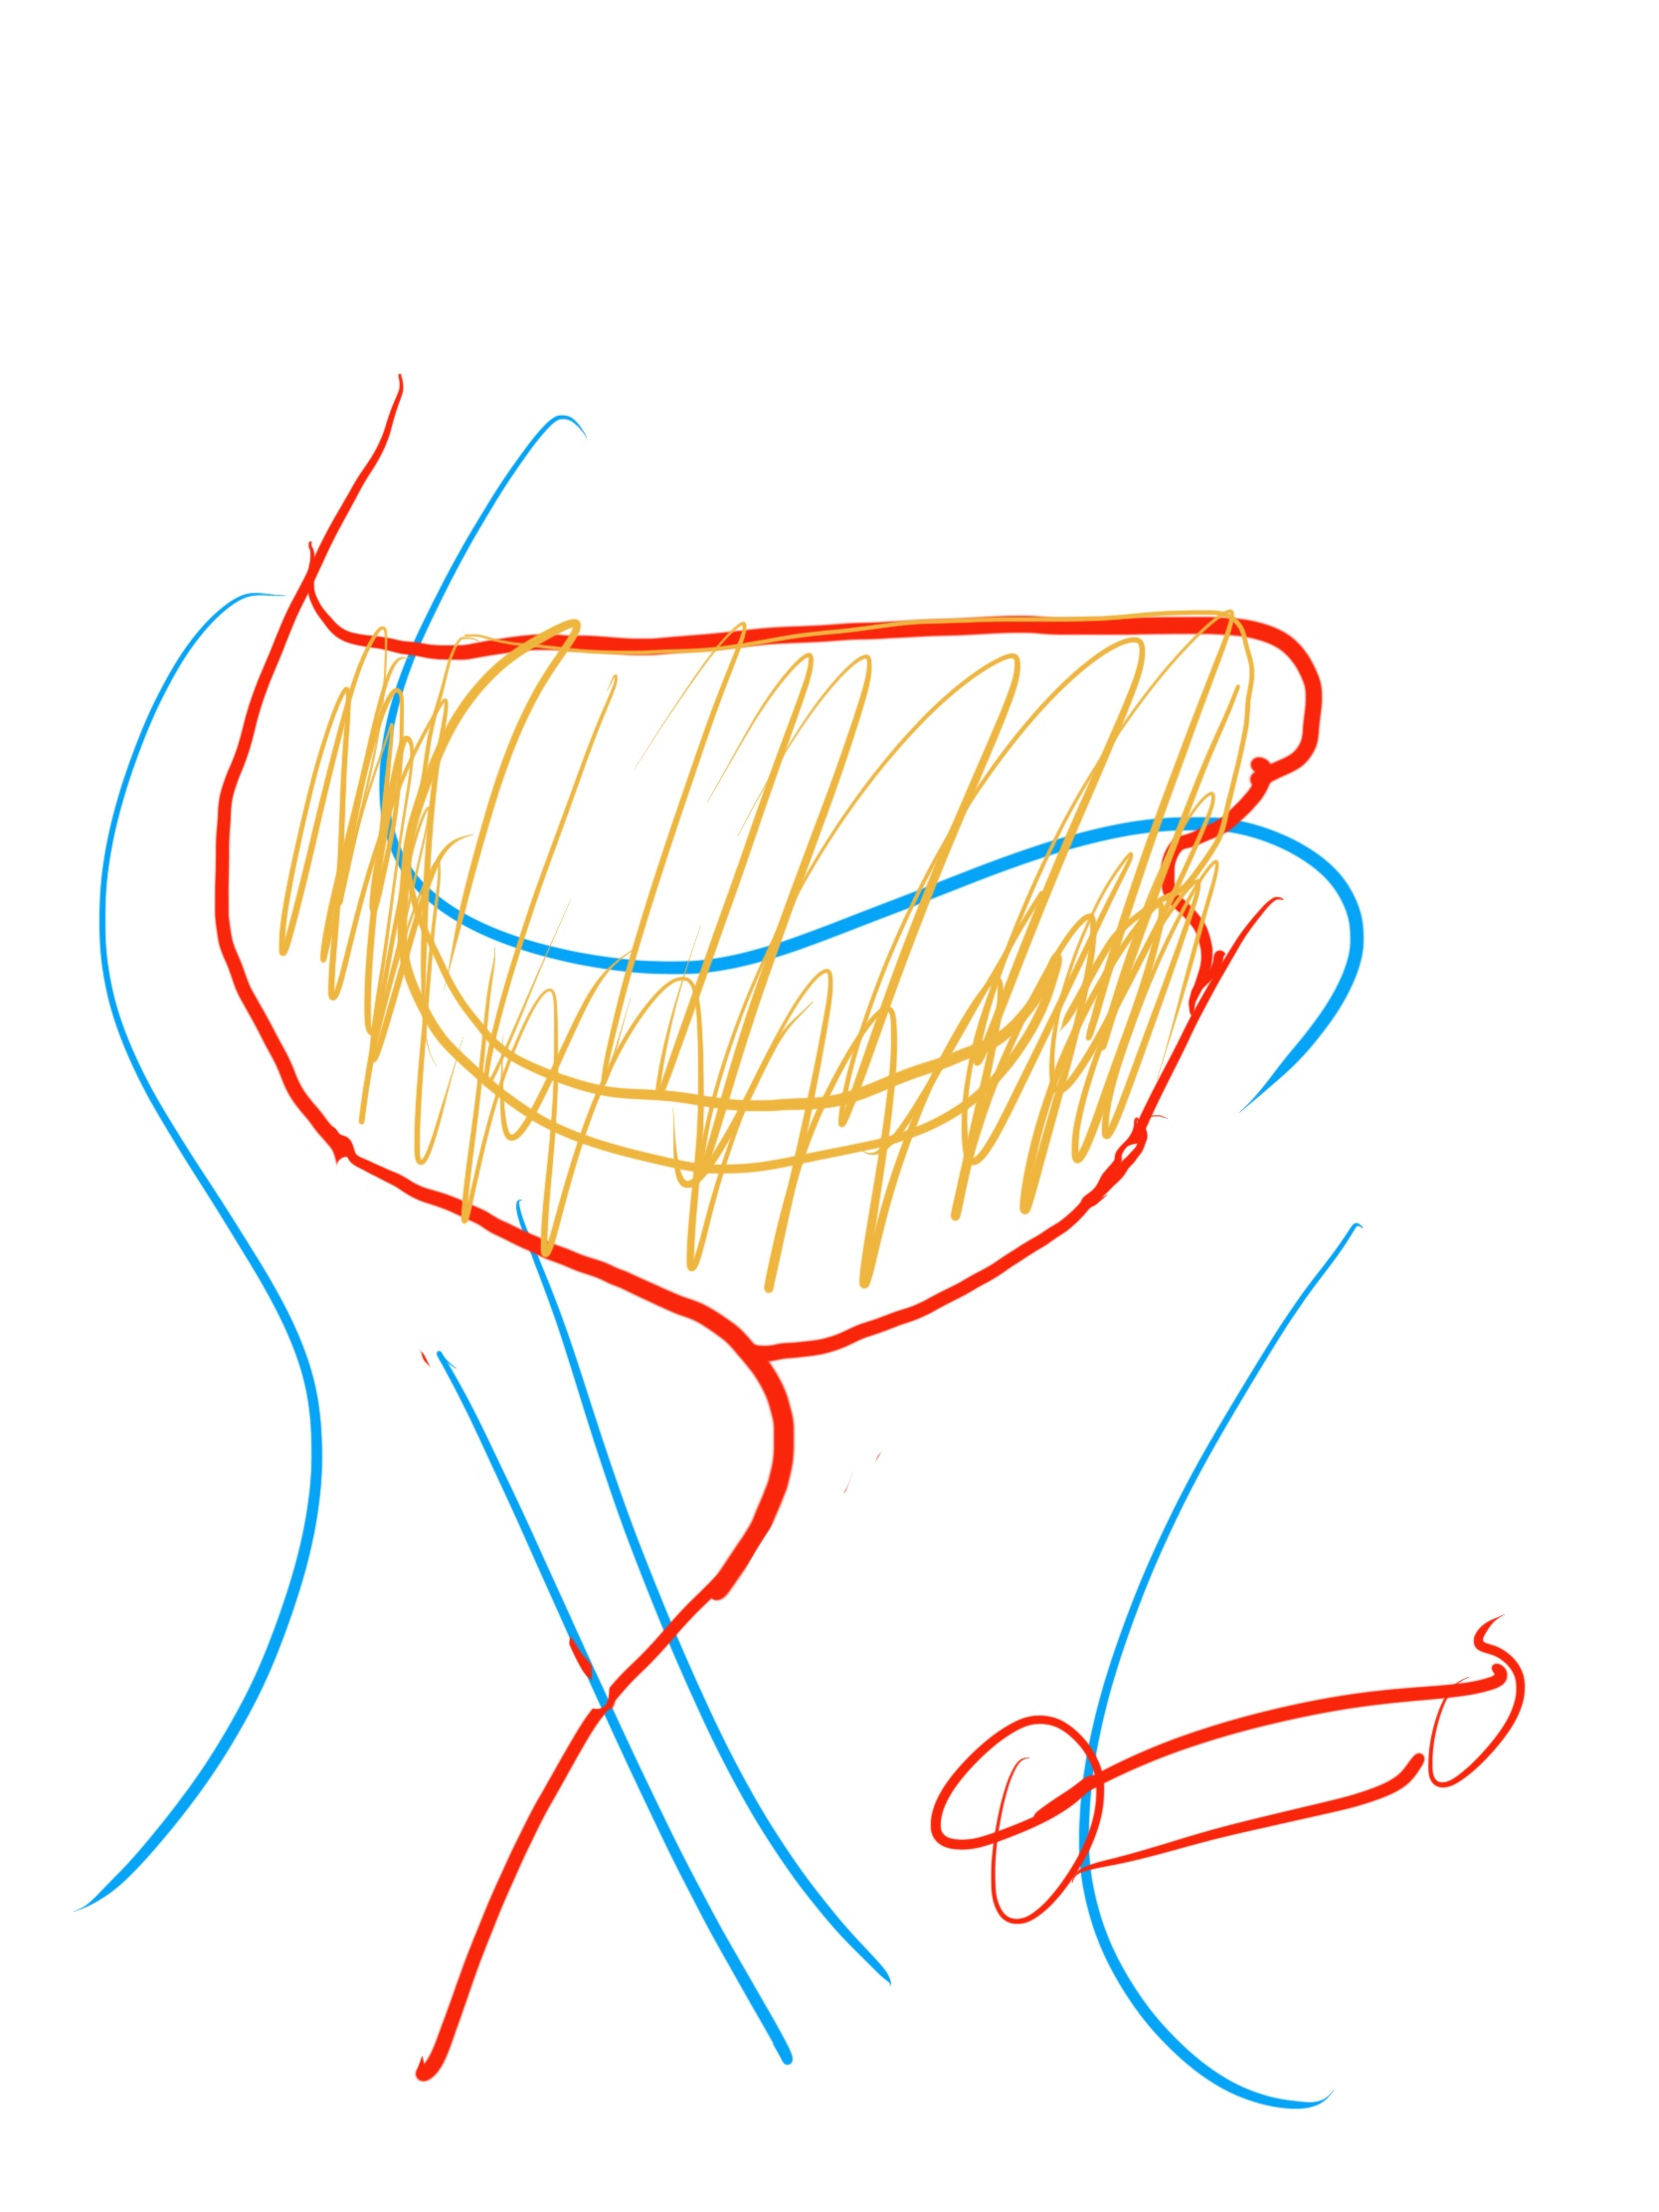
\includegraphics[width=3.5cm]{SOHND_Artwork.jpg}
\end{figure}



\clearpage

%%%%%%%%%%%
\thispagestyle{headings}
\markright{Introduction\hfill We do HNSCC therapy \hfill}

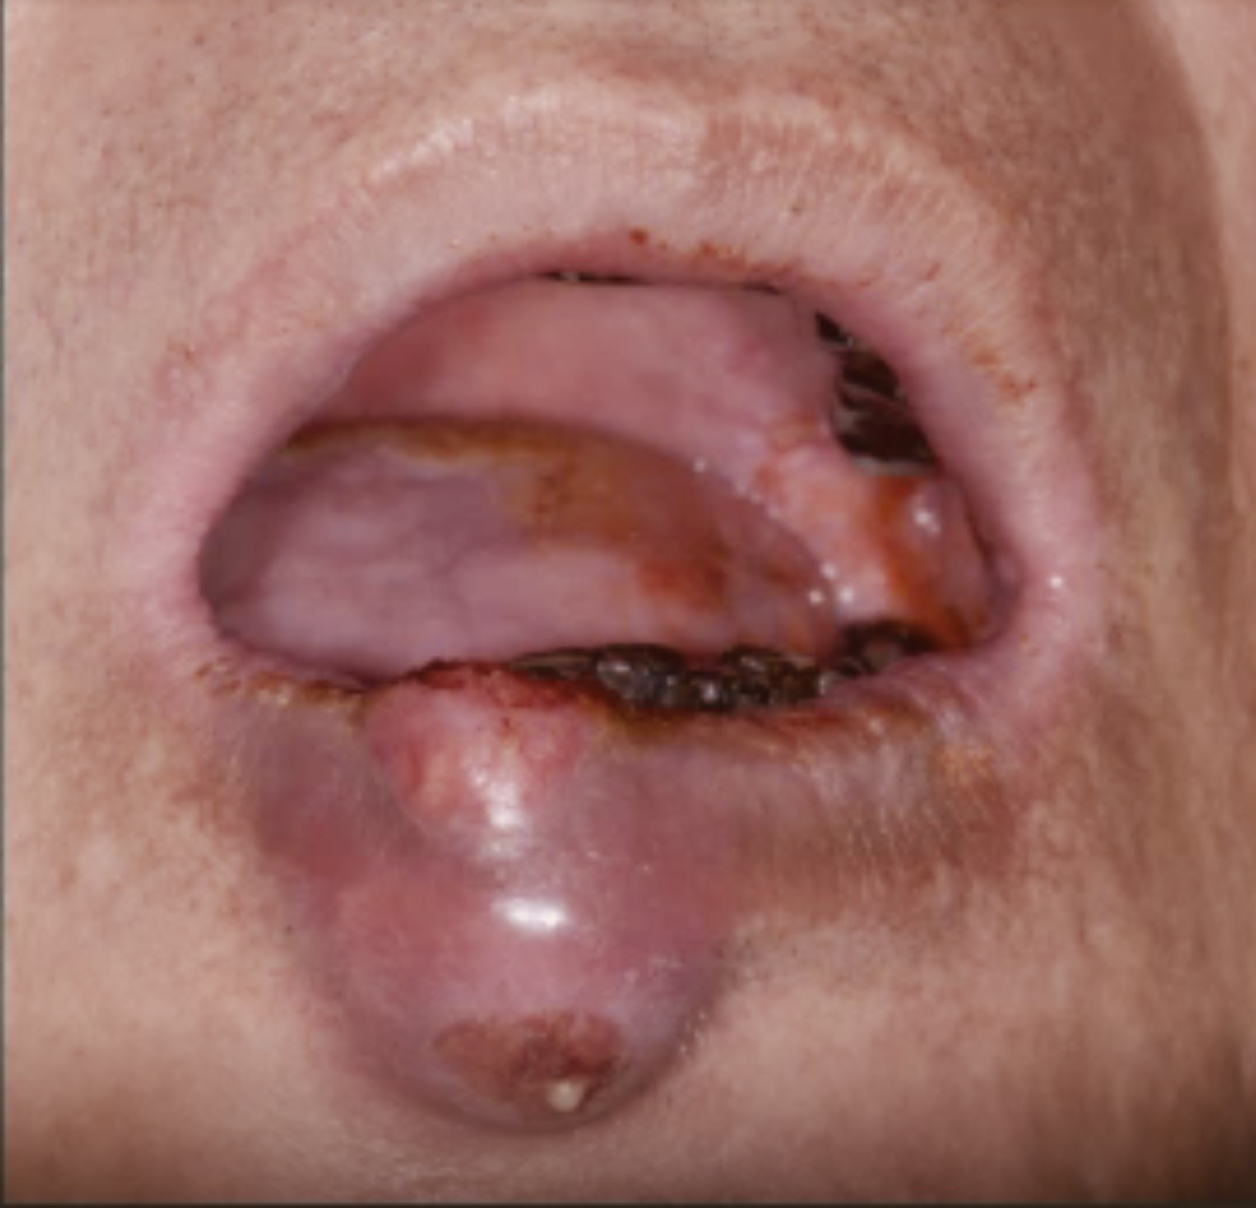
\includegraphics[width=2cm]{IMG_7174.jpg}
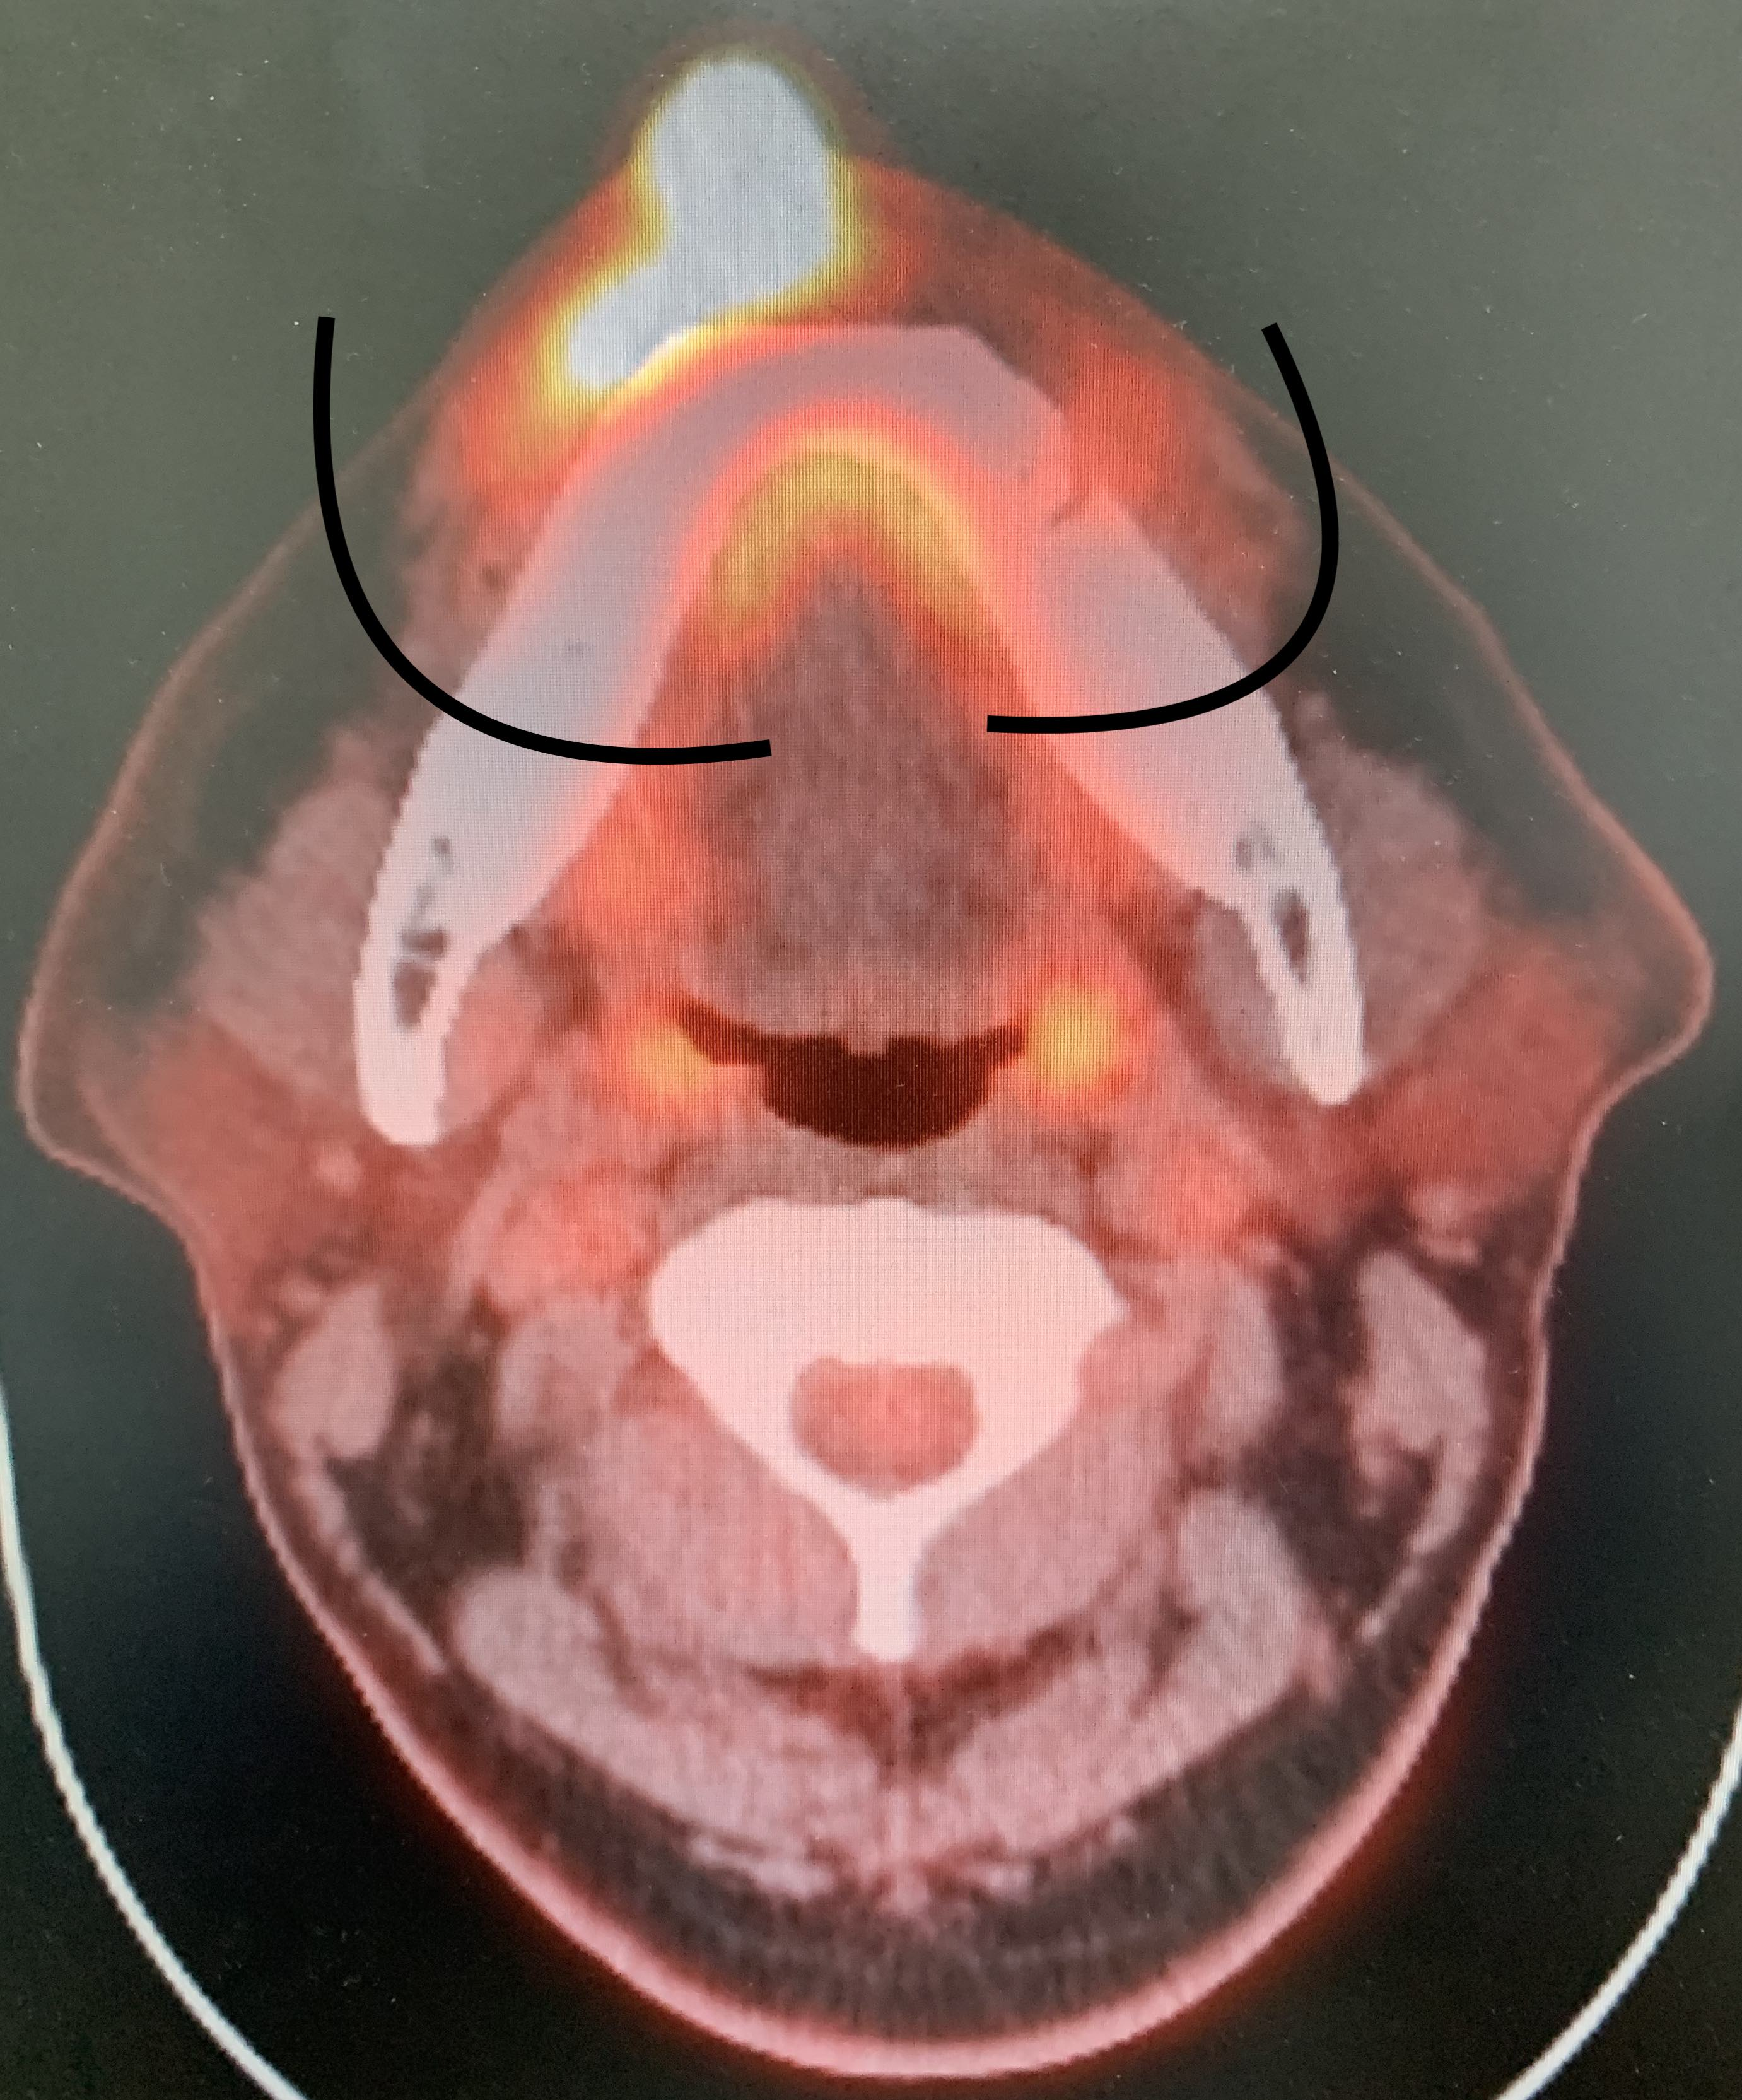
\includegraphics[width=4cm]{IMG_6430.jpg} % PET/CT scan
%\begin{figure}[!h]
%    \centering
%    \caption*{(Image courtesy of Guatacara et al., 2018)}
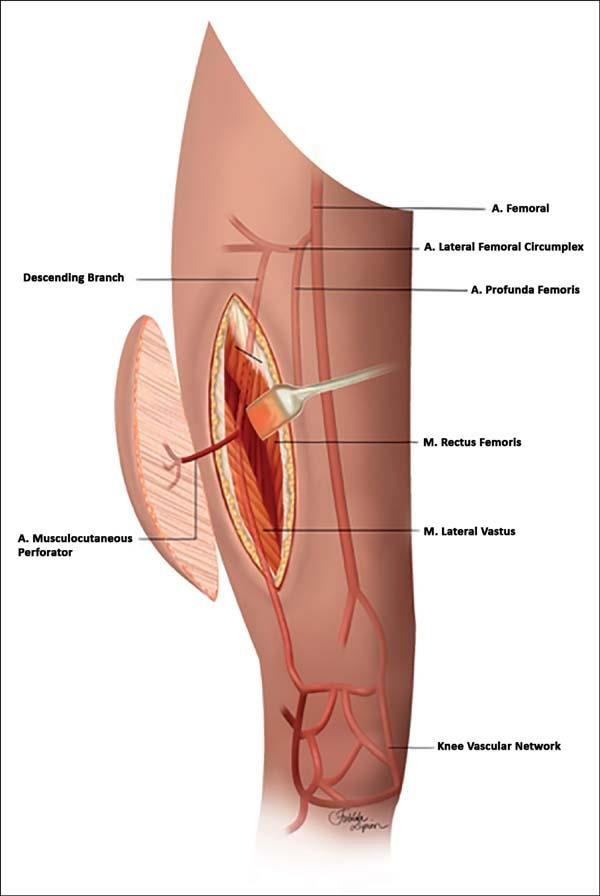
\includegraphics[width=4cm]{Figure-5-Vascular-anatomy-of-ALT-flap-Guatacara-et-al-2018_W640.jpg}\\
\large Wide excision (cut on black line) with selected neck (lymph nodes) dissection\\
\hspace{2cm} 
{\tiny (The illustration courtesy of Guatacara et al., 2018) \par}


% https://www.researchgate.net/publication/337208414_Anterolateral_thigh_versus_radial_forearm_free_flaps_in_reconstruction_of_oral_cavity_malignant_defects/figures?lo=1
%\end{figure}
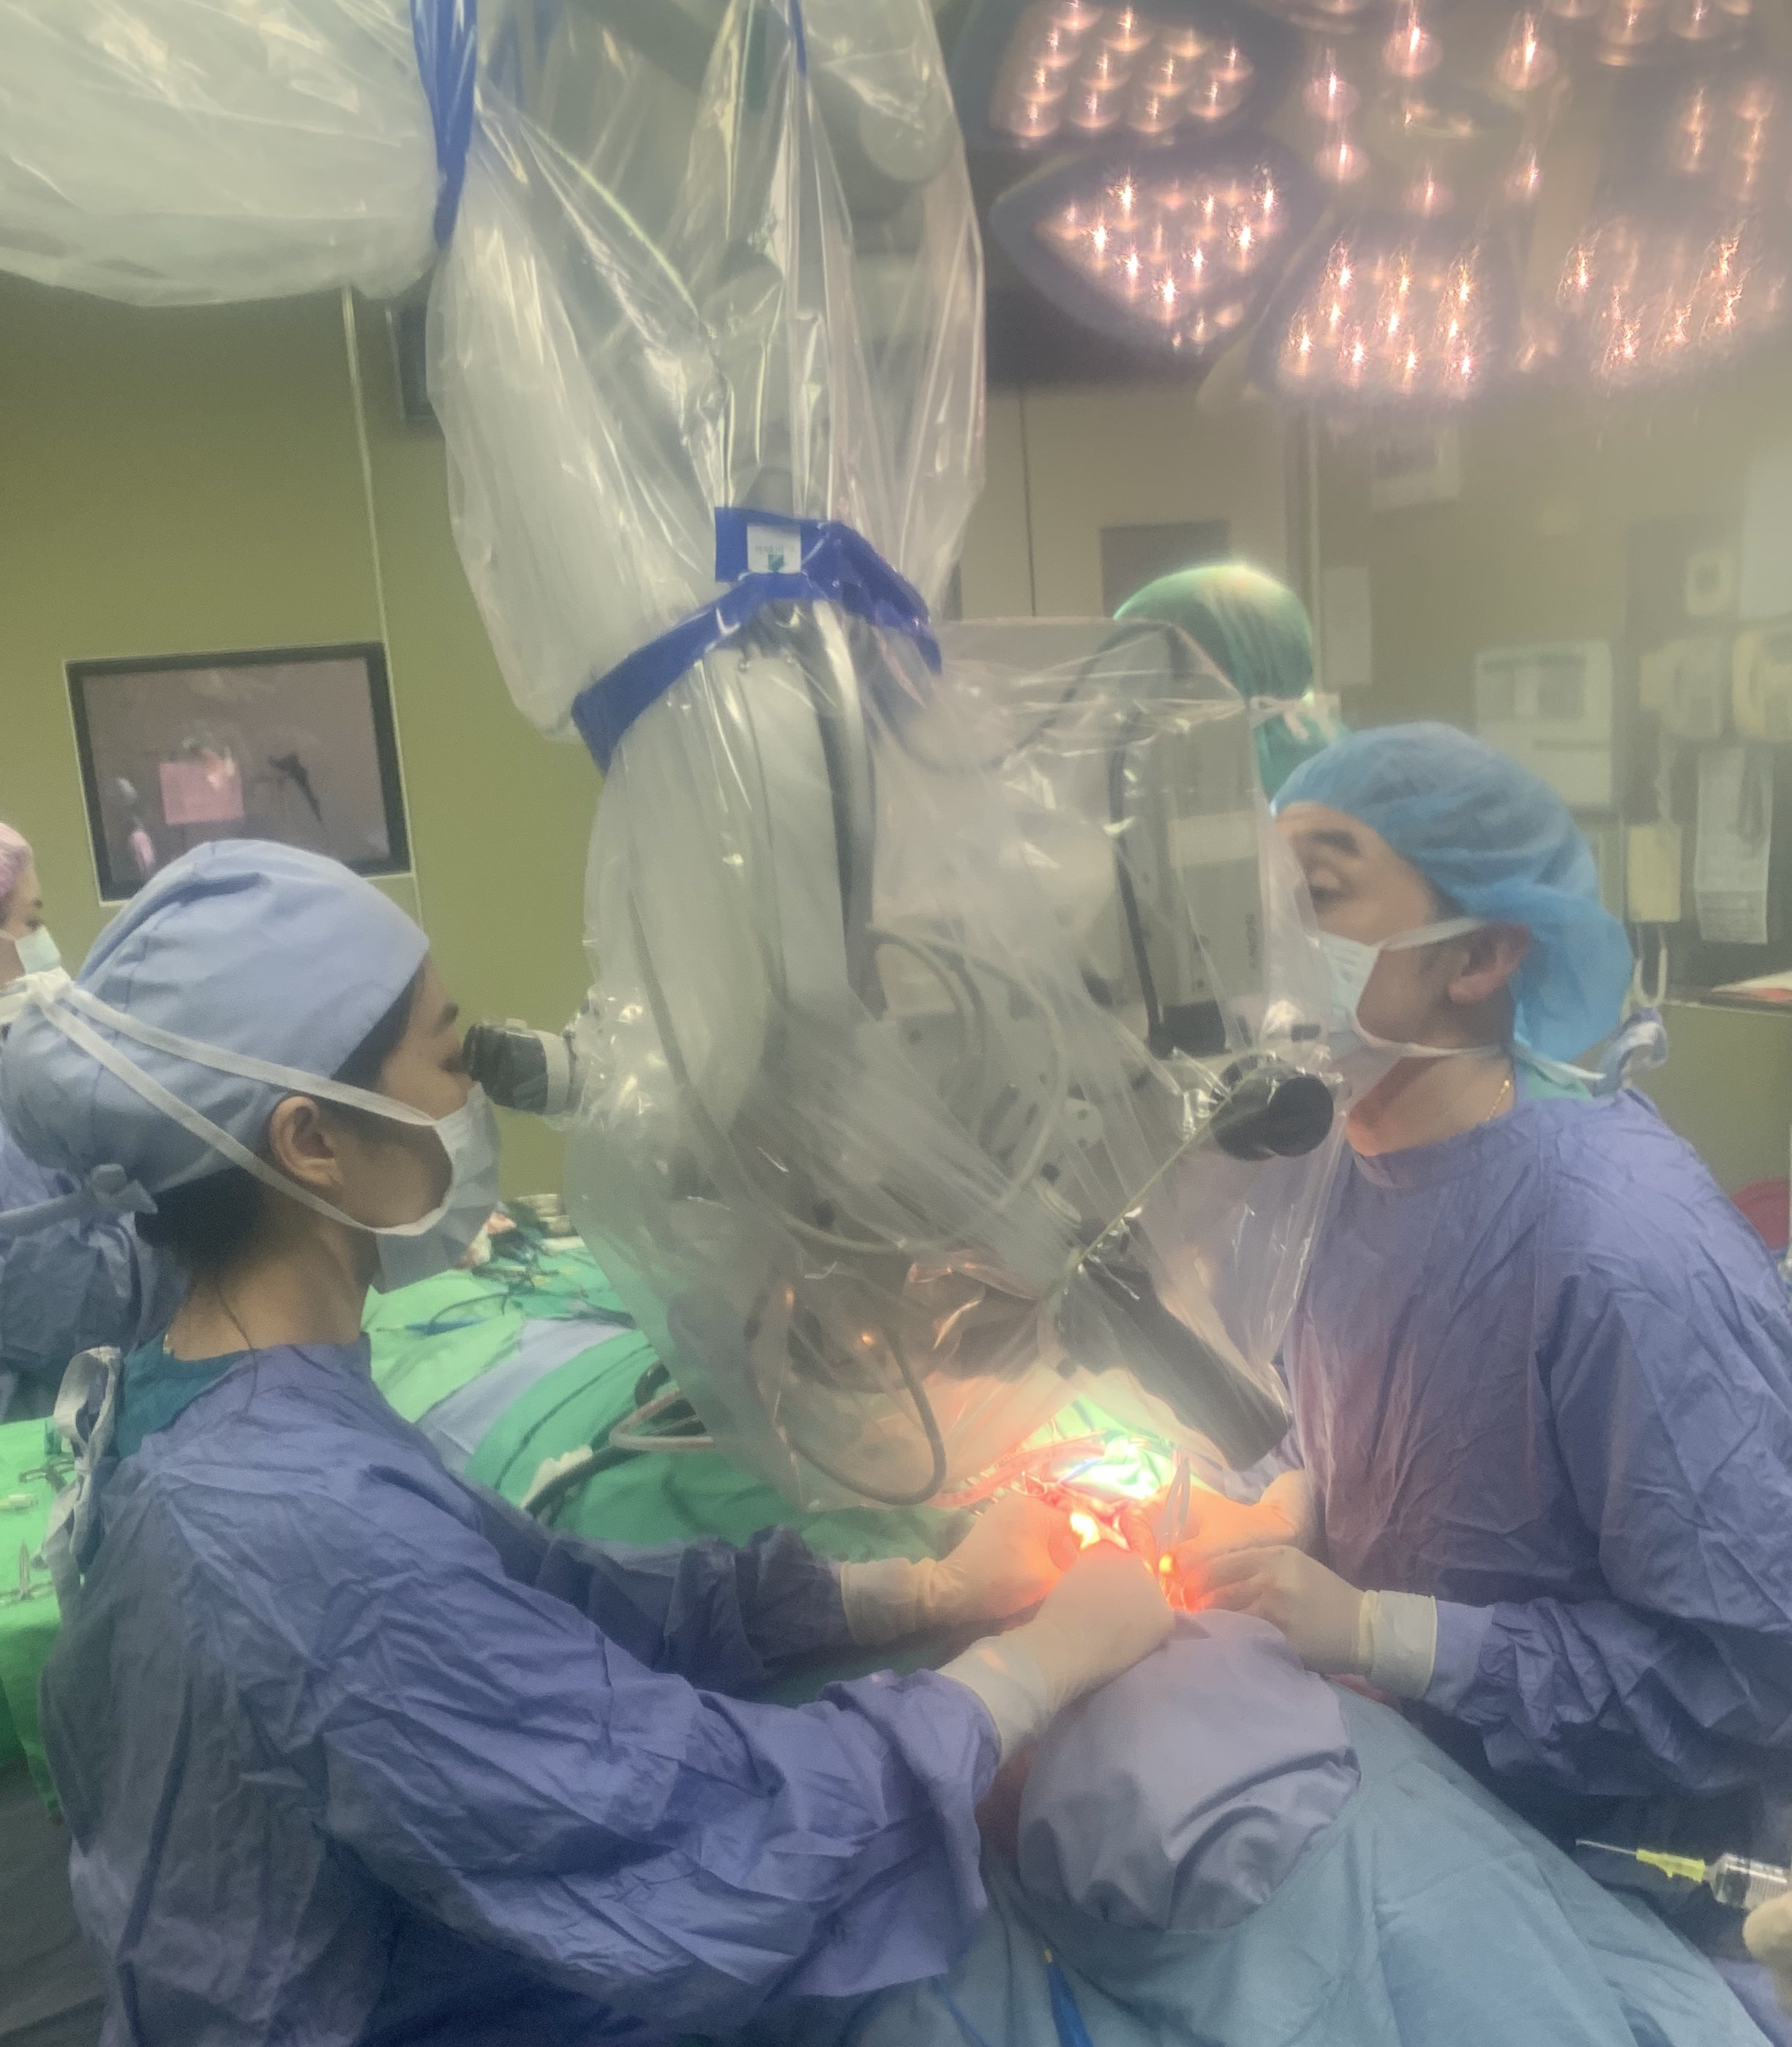
\includegraphics[width=5cm]{IMG_6791.jpg}
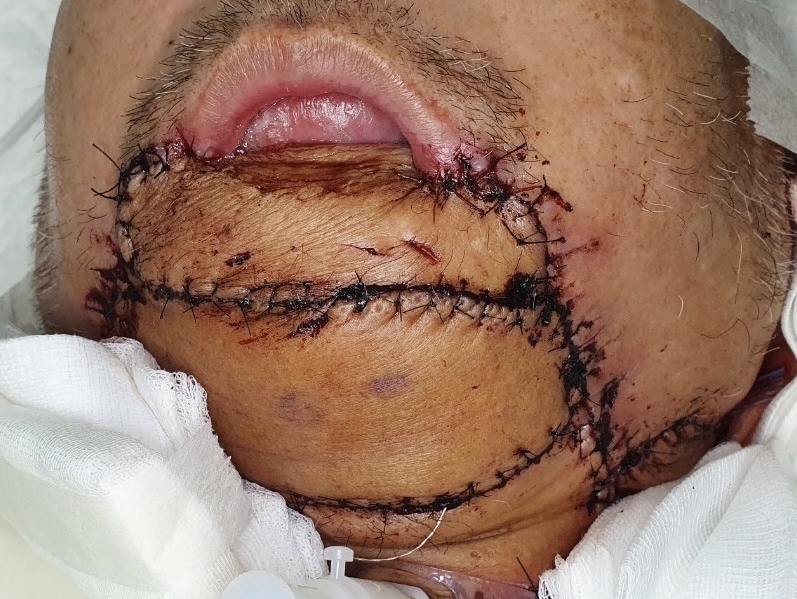
\includegraphics[width=6cm]{IMG_6910.jpg}\\
\large Reconstruction with free flap (tissue transfer) under micro-surgery team\\
{\tiny (Photos courtesy of TMU team: Dr. CY Wu and Dr. Evienne Hong on 2021/11/17)}

\clearpage
%% f/u 2009 to 2021 our thinking process: biomarker, screening TCGA, deep learning and holistic
\thispagestyle{headings}
\markright{Introduction\hfill We do HNSCC research \hfill}

\large Since surgery, we follow patients up closely, and they are always \hl{anxious} about their \hl{recurrence} (so do I).\vspace{5mm}

\begin{outline}
\0 The ways we do for improving our confidence of their prognosis, by
\1 biomarkers discovery from \hl{(A) proteomics} and \hl{(B) transcriptomics} research:
    \2 (A) the in-house HNSCC datasets (in vitro, in vivo)~\parencite{Chi2017};
    \2 (B) the public \acrfull{rnaseq} databases (in silico)~\autocite{Chi2021};
\1 investigation of \hl{surgical margin} (T) and \hl{neck metastasis} (N) by deep learning algorithm (grant proposal);
\1 development of \hl{holistic} cancer care in Taipei Medical University affiliated Hospitals.

\end{outline}
\clearpage
%%


\comm{
%%
%%% Chi2017 %%%%%%%%%%%%%%%
\section{Materials and Methods for (A) Proteomics} % 4

\subsection{Hypothesis for Chi2017} 
\begin{outline}

% top-down 
%\1 A proteomics research
\1 Biomarkers according to 
    \2 differential gene expression (protein) between normal (N) versus tumor (T) tissue
%    \2 spatial distribution on pathological slides, 
    \2 distribution on cancer stage (e.g., I II III or IV; by TNM system);
\end{outline}

\clearpage
\subsection{Two Patient Cohorts}
% KGVH and TMU cohorts for TMSB4X

\large The \acrfull{hnscc} specimen from Kaohsiung Veterans General Hospital (KVGH): n = 35, for \hl{mass spectrometry}\\ %528\\ discovery cohort
\indent{\acrfull{tmuh} cohort: n = 86, for \hl{survival analysis}}%288 validation cohort

%\subsubsection{RNA Sequencing Data} 
%20,500 \hl{RNA-Seq} data of protein-coding genes\\%, derived from cancer specimen of each participant


\subsubsection{The Clinicopathological Data}
gender, age, tumor size (T), cervical lymph node metastases (N), and \hl{overall survival data}.
%distant metastasis (M), \hl{pathological surgical margin}, tobacco exposure

%\tiny * \acrfull{rest}

\clearpage
%\subsubsection*{Demographic data}
% a table
% Please add the following required packages to your document preamble:
% \usepackage{graphicx}
%\begin{table}[H]
%\centering
%\caption{}
%\label{tab:my-table}


%\end{table}

%\clearpage





%%%%%%%%%%%%%%%%%
% automatic generation by jpm2KOMO-script.py
%% [2011/08/08]
%%%%%%%

%\section{Materials and Methods}

\thispagestyle{headings}
\markright{Materials and Methods for (A)\hfill Proteomics Workflow \hfill}

\begin{figure}
  \begin{minipage}[c]{0.35\linewidth}
  \begin{picture}(15, 20) % zero point at left end/H mid-line of (15,20) %(1,0.55038404)%
\centering
  \put(5,-65){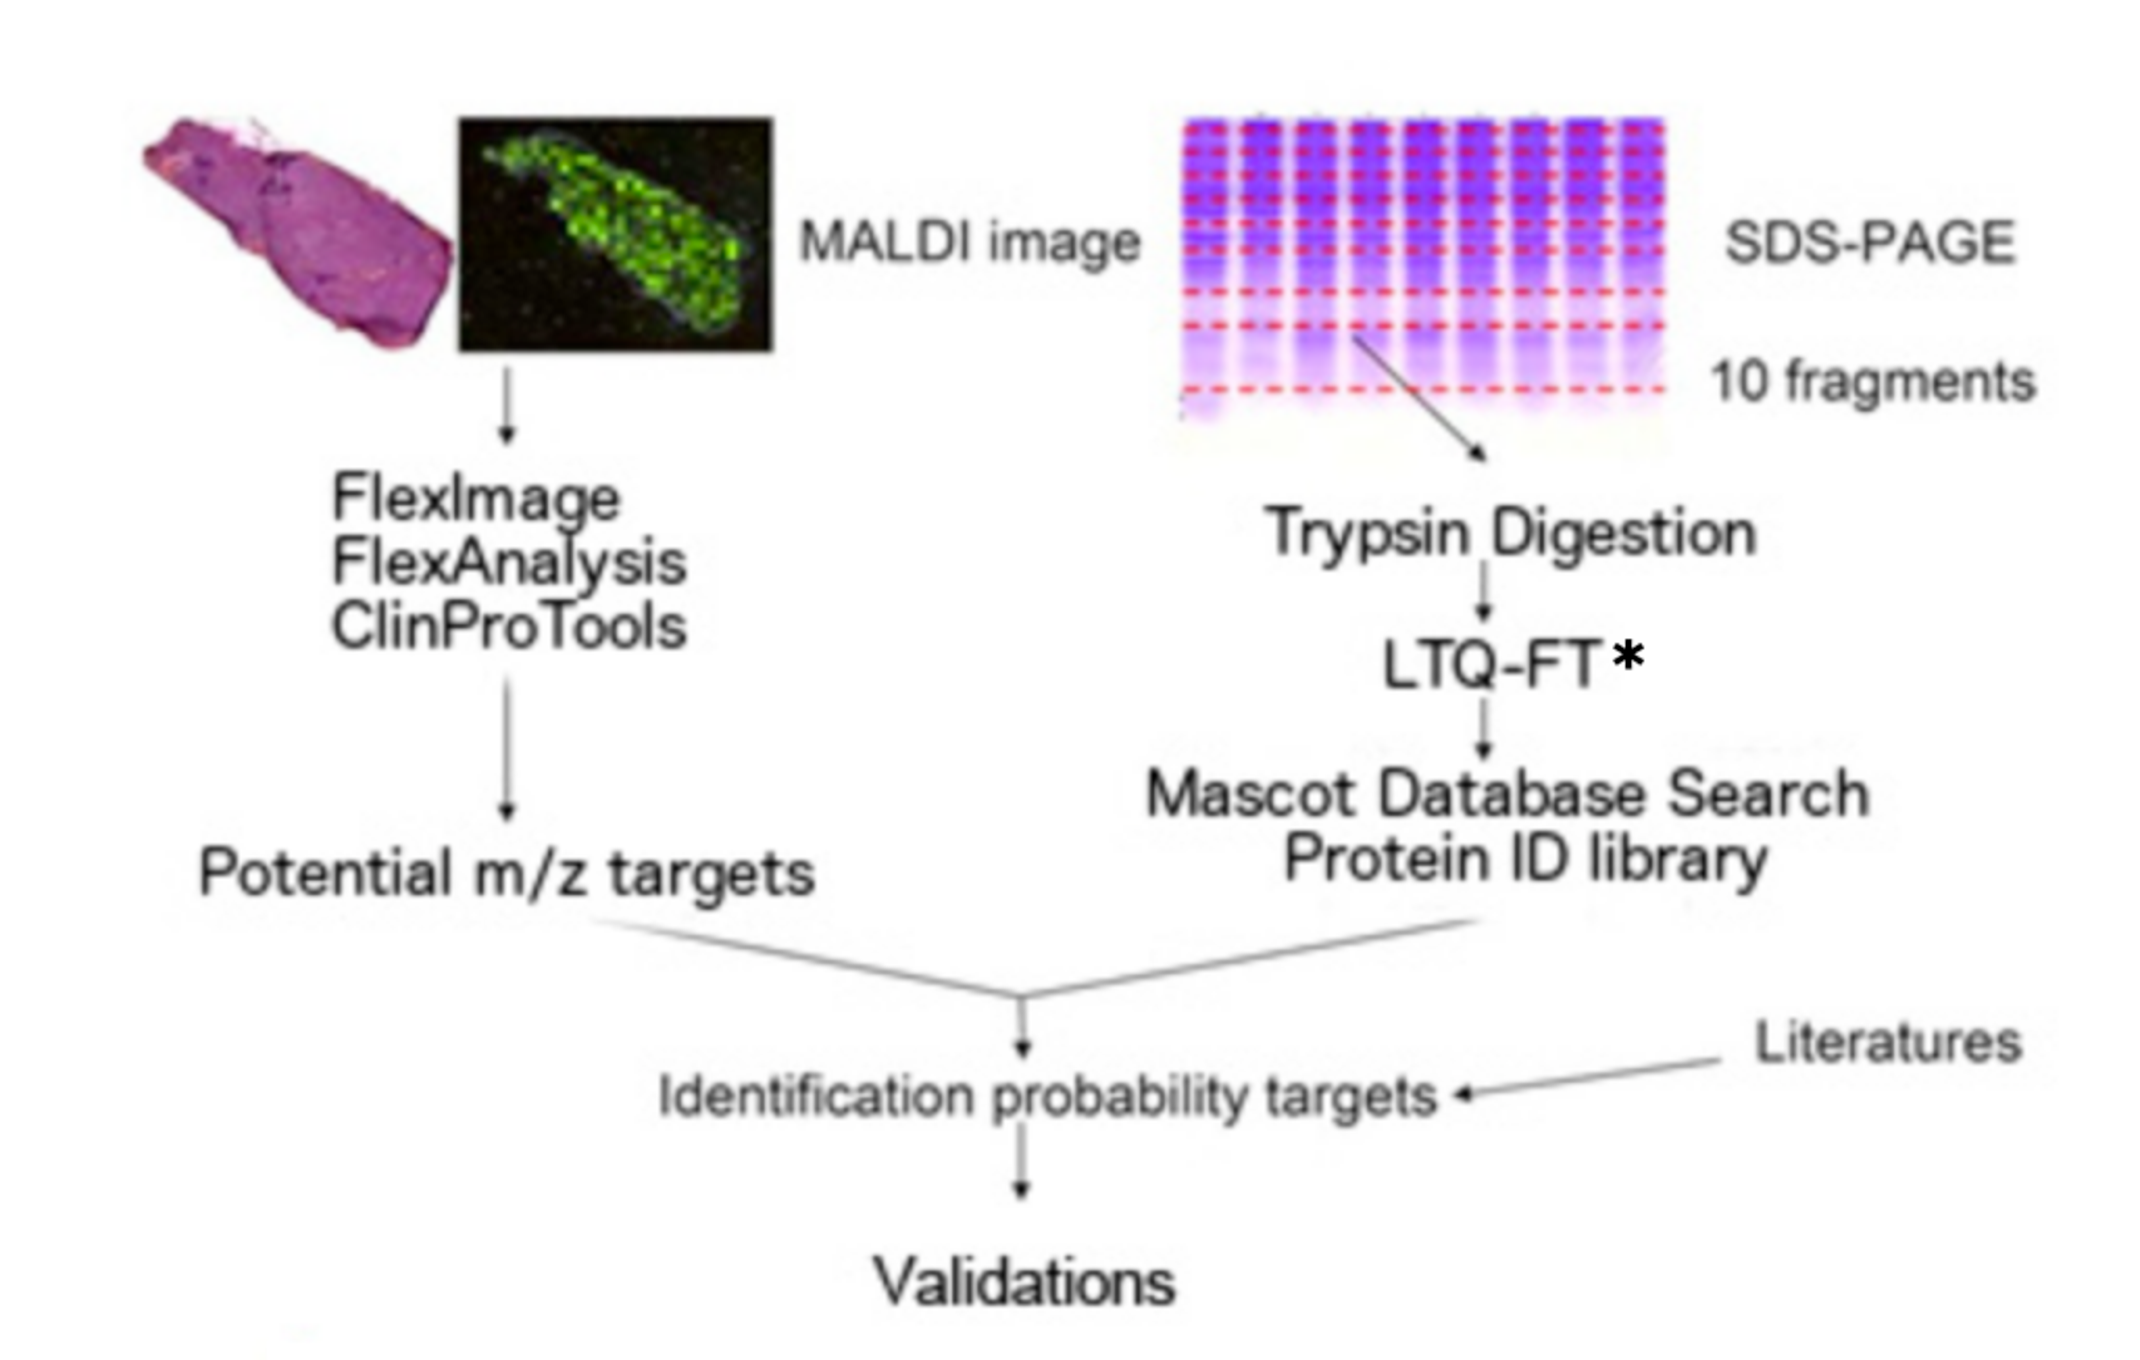
\includegraphics[width=7.0cm]{Figure-1_MALDI_Hsiao_A.PDF}}
  %graphic_abstract_pvalueTex.pdf}}% X-axis: hyphen to minus sign
%    \includegraphics[height=7.0cm, width=7.5cm]{graphic_abstract_pvalueTex.pdf}%
    \captionsetup{labelformat=empty}
%    \caption{Figure. Mindfulness meditation in \hl{holistic} cancer care}
  \put(45.5, 63.5){%\fontfamily{qcr}\selectfont
  \large (1)}
  
  \put(132.5, 63.5){%\fontfamily{qcr}\selectfont
  \large (2)}
%  \put(178.5, 48.5){%\fontfamily{qcr}\selectfont
%  \large (2)}
%  \put(188.5, 10){%\fontfamily{qcr}\selectfont
%  \large (3)}
%  \put(178.5, -10){%\fontfamily{qcr}\selectfont
%  \large (4)}
  \put(92.5, -25){%\fontfamily{qcr}\selectfont
  \large (3)}
  \put(70, -60){%\fontfamily{qcr}\selectfont
  \large (4)}
%  \put(2,-105){Figure. Overview of the strategy used for identification of the biomarker in \acrshort{hnscc}}
  %Mindfulness meditation in \hl{holistic} cancer care}
  
  \end{picture}
  \end{minipage}\hfill
  \begin{minipage}[c]{0.55\linewidth}
    \centering
    \begin{outline}[enumerate]
   % \0 Workflow for identification of the biomarker in \acrshort{hnscc}
        \1 Profiling of proteomes from \hl{pathology slides} of KVGH cohort by \acrshort{maldii} {\tiny (\acrlong{maldii})}
        % with ClinProTools analysis
        \1 Construction of protein library from normal oral cell and cancer \hl{cell lines} by \acrshort{lcms} {\tiny (\acrlong{lcms})}
%            \2 in-gel digestion (peptide) $\longrightarrow$
%            \2 separation by liquid chromatography (LC) $\longrightarrow$
%            \2 analysis by linear ion trap quadrupole (\textcolor{red}{LTQ}) mass spectrometer combined with a Fourier transform-ion cyclotron resonance (\textcolor{red}{FT-ICR}) mass spectrometer (LTQ--FT MS/MS, Thermo Electron) % a kind of tandem mass spectrometer
%        \1 \hl{sliding-window} cutoff mining engine for Kaplan--Meier survival analysis to find a optimal cutoff
%        \1 Candidate selection
%        \1 Biomarker validation

    \end{outline}
%    \captionof{table} % by KOMA-script
%      {%
%        Different kinds of ducks%
%        \label{tab:duck}%
 %     }
  \end{minipage}
\end{figure}




\clearpage




\thispagestyle{headings}
\markright{Statistics \hfill Differentially expressed genes (DEGs) analyses for KVGH cohort  \hfill}%\hfill Why TCGA dataset? \hfill}

\subsection{MALDI Imaging}
% Cutoff Finder Core Engine

%\subsection{Statistical Consideration for Survival Analysis}
\begin{minipage}[c]{0.65\linewidth}
%\large
\begin{outline}
%\1 peptide mass fingerprint
\1 \acrfull{maldii} has spatial information
\1 tissue slide (normal, stage I II III IV)
\1 softer ionization of \hl{whole molecule}
\1 detection up to 100,000 Dalton (molecular weight) of protein
%\1 recording mass-charge ratio (m/z)
% Essentially, the Bruker Daltonics Ultraflex consists of two Time-of-Flight channels. The first separates the ions generated by laser beam on the basis of their molecular weights giving a mass fingerprint. The second TOF resolves the fragmented species generated by a collision chamber, which is present between the two TOFs. We have been able to fragment peptides (generated from tryptic digests of proteins) of upto 3000 Da and the fragmentation of higher mass peptides is being standardized. We also carry out routine mass determination of proteins with molecular weights as high as 80 kDa. The accuracy of the instrument is about 0.1 Da in the low molecular weight range (upto 8 kDa) and drifts to about 5-20 Da when the mass range hits the 75 kDa range, depending on the laser power employed. Theoretically, the upper limit of the mass detection range is set at infinity. However, we have been having problems getting large molecular weight proteins (about 90-120 kDa) to ionize well.
\end{outline}
\end{minipage}
\begin{minipage}[c]{0.25\linewidth}
    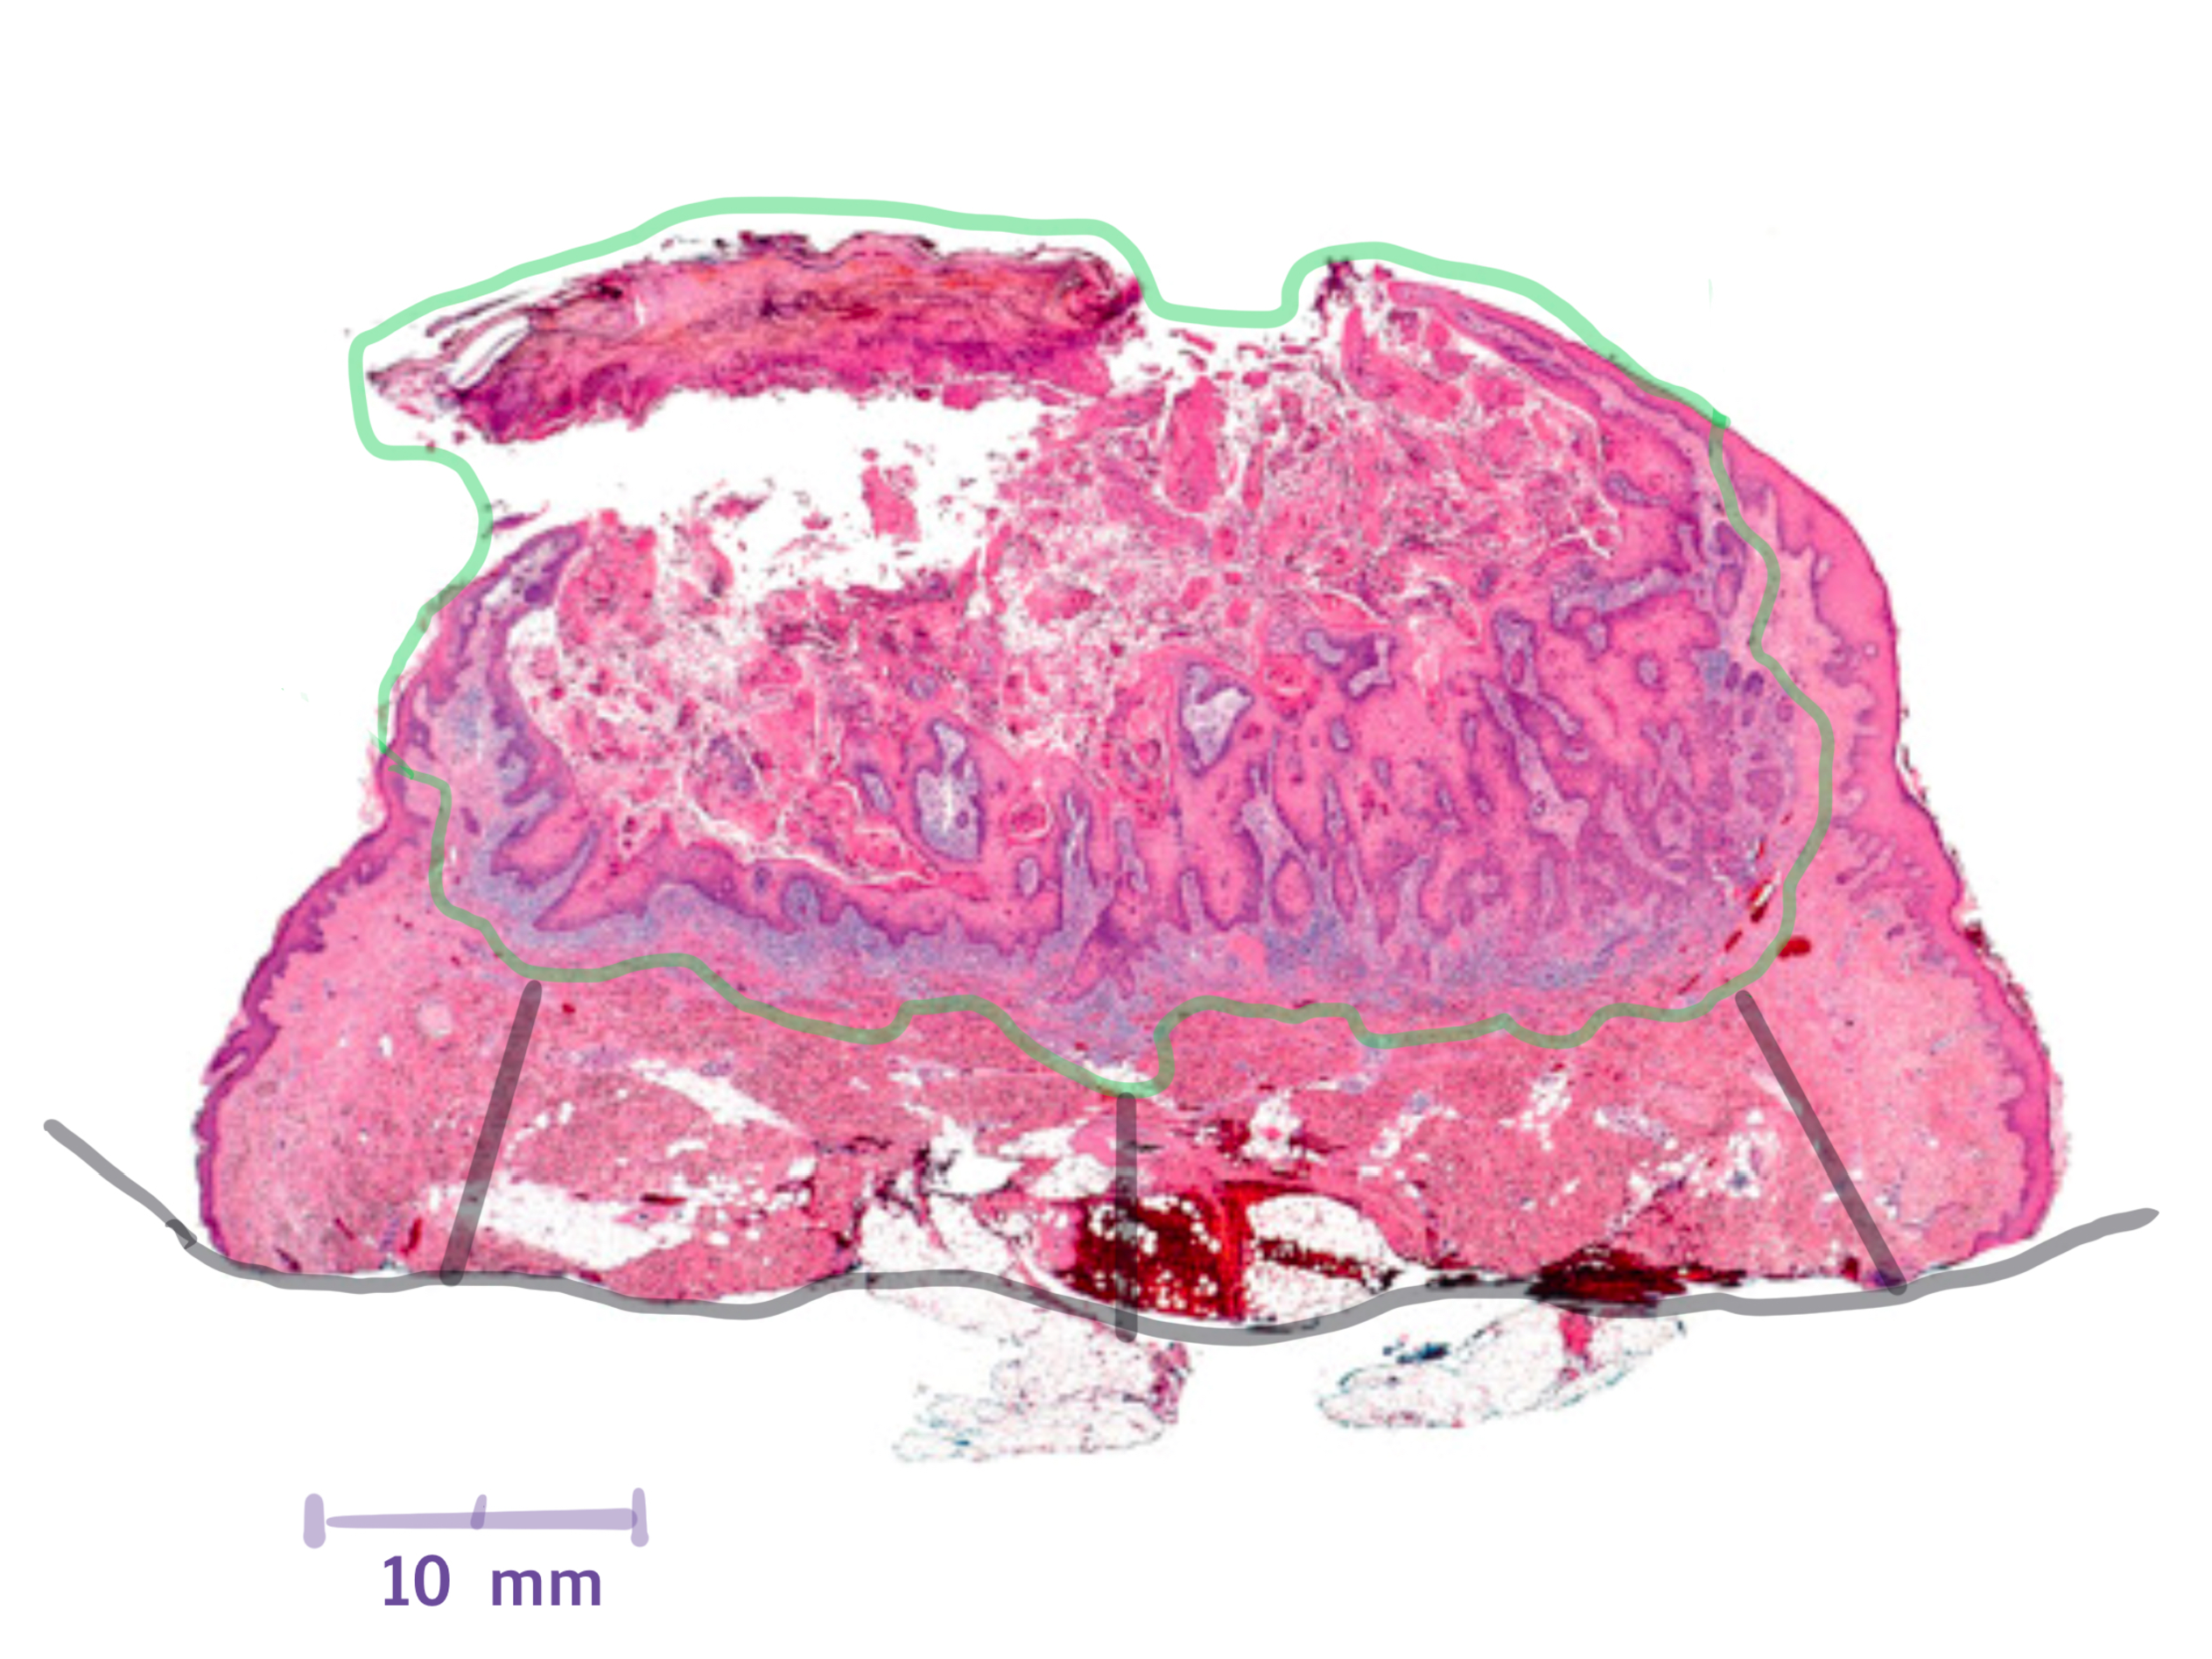
\includegraphics[width=4cm]{GCNN_for_surgical_margin_HE.pdf}
{\tiny Whole-slide pathological image of HNSCC (courtesy of Dermatology, 2017, 4th Ed.~\autocite{Bolognia2017} )}
% Bolognia2017 \cite{Bolognia2017} Bolognia_Jean_L_2017-10-22
\end{minipage}




\clearpage
%%
\begin{minipage}[c]{0.65\linewidth}
%MALDI: 分離、純化不易揮發、不能加熱的化合物 蛋白質 from tissue slide (frozen sectioned)
%LC: 分離 peptide from cell lines
%GC: 分離、純化易揮發、熱穩定性佳化合物
\begin{outline}
% why TOF: https://www.tofwerk.com/advantages-time-of-flight-mass-spectrometry-over-quadrupole-ms/
    \1 UltraFlex MALDI-TOF/TOF* (Bruker Daltonics) with a 337-nm nitrogen UV \textcolor{red}{laser} operated at 0.5-20 ns pulse duration
    {\tiny (*TOF: Time-of-Flight mass spectrometer)}
    \1 scanning \textcolor{red}{200 squares} (x 500 laser shots) in each tissue slice $\longrightarrow$ 100,000 shots per slide
    \1 protein sorting by mass-to-charge ratio (m/z) with TOF mass spectrometer (MS1)
    \1 protein detection by mass-to-charge ratio (m/z) with TOF mass spectrometer (MS2)
\end{outline}
\end{minipage}
\begin{minipage}[c]{0.25\linewidth}
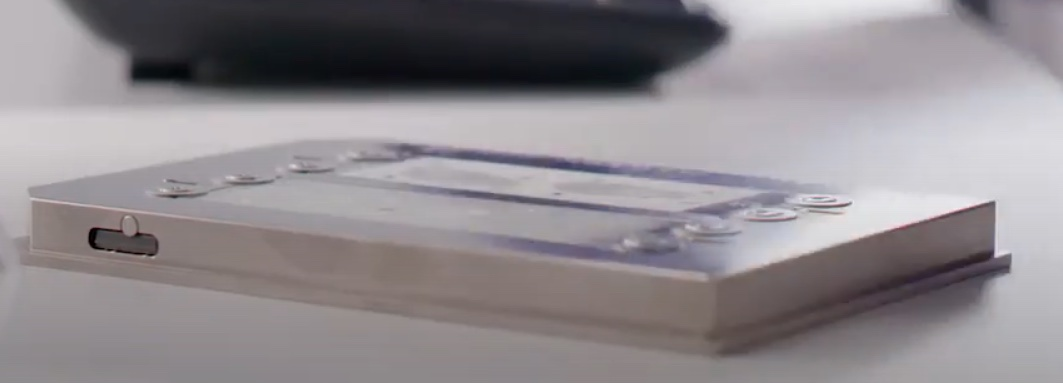
\includegraphics[width=4cm]{MALDI_image_slide.jpg}
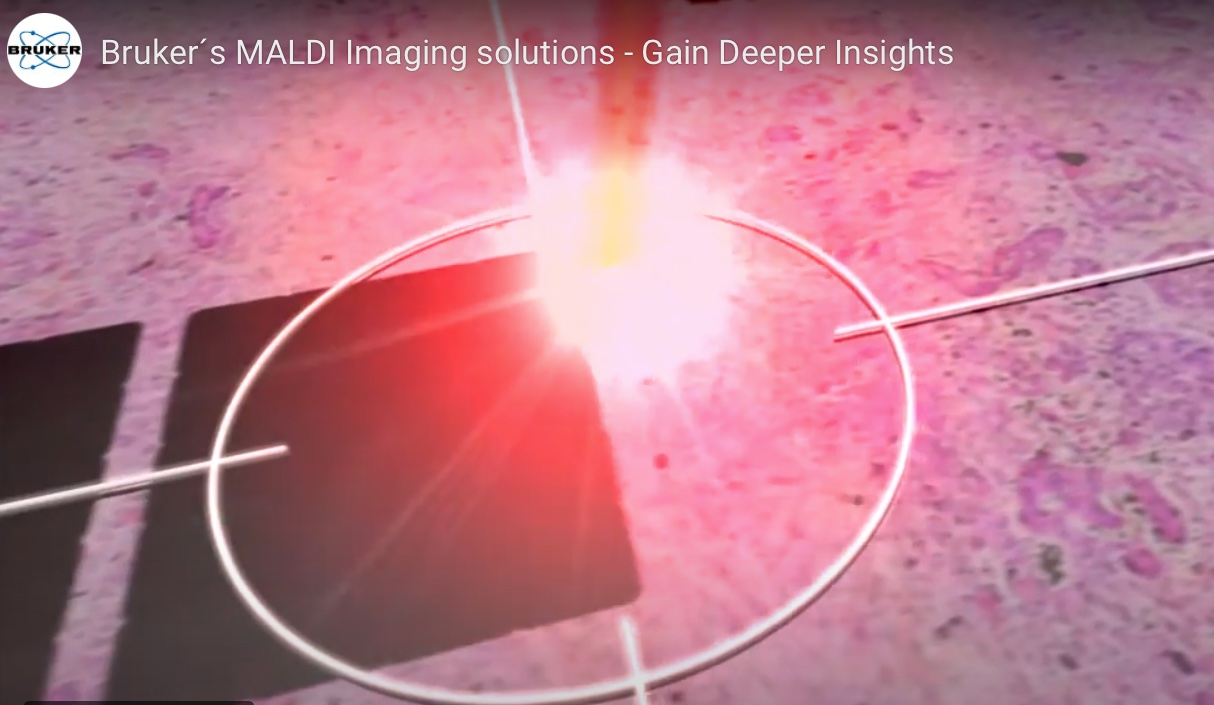
\includegraphics[width=4cm]{MALDI_image_demo.jpg}
{\tiny Image courtesy of Bruker Daltonics}
%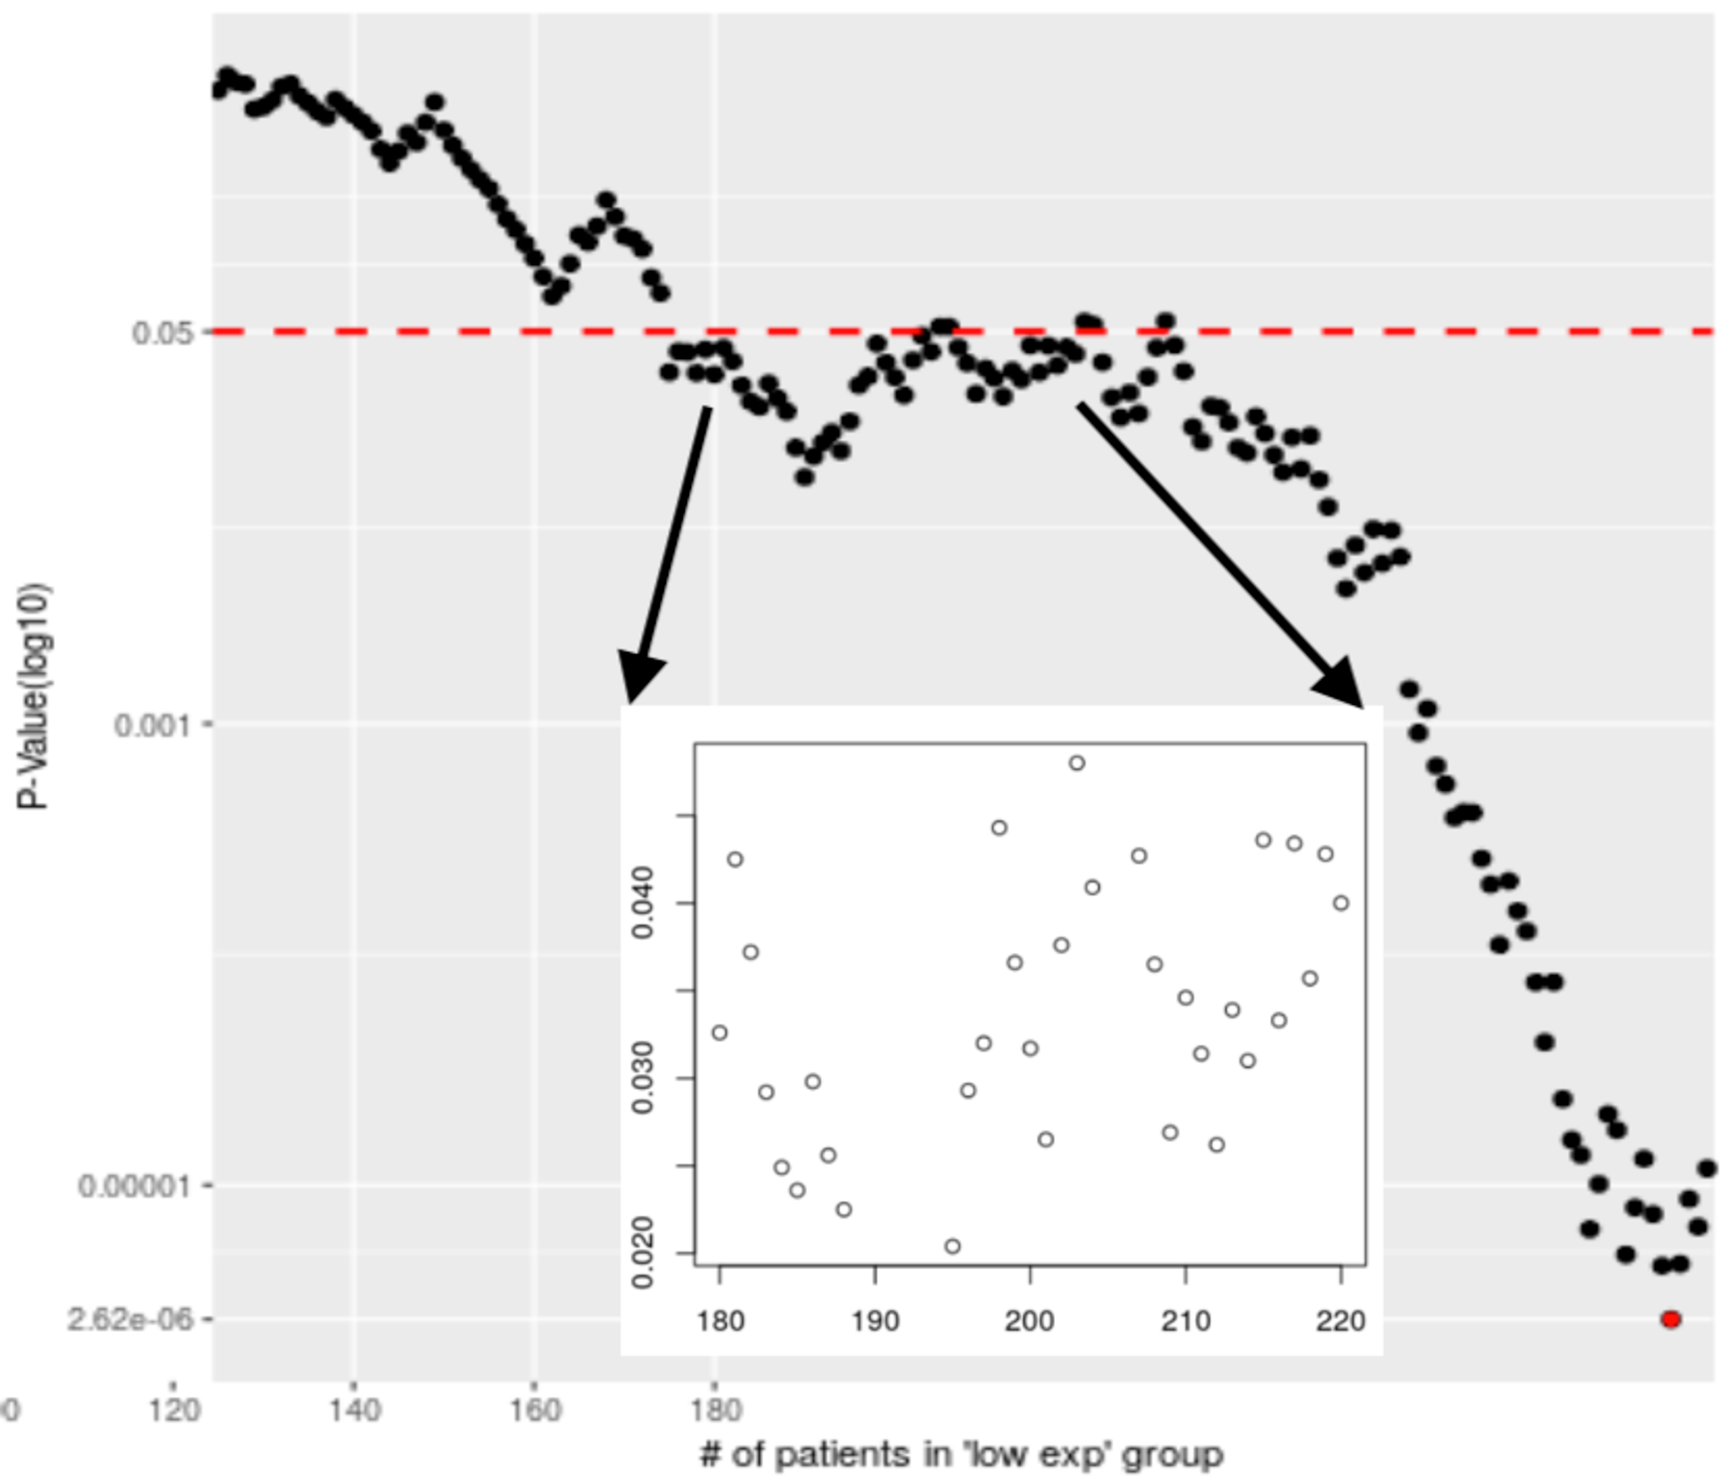
\includegraphics[width=3cm]{Rplot_pvaluePlot_NDFIP1.pdf}
\end{minipage}
\clearpage

%%
\begin{minipage}[c]{0.65\linewidth}
\begin{outline}
    \1 Spectra made by flexImaging,  flexAnalysis and ClinProTools
    \1 Quantification (DEGs) of tumor versus normal tissue by classification model of genetic algorithms and support vector machine
\end{outline}
\end{minipage}
\begin{minipage}[c]{0.35\linewidth}
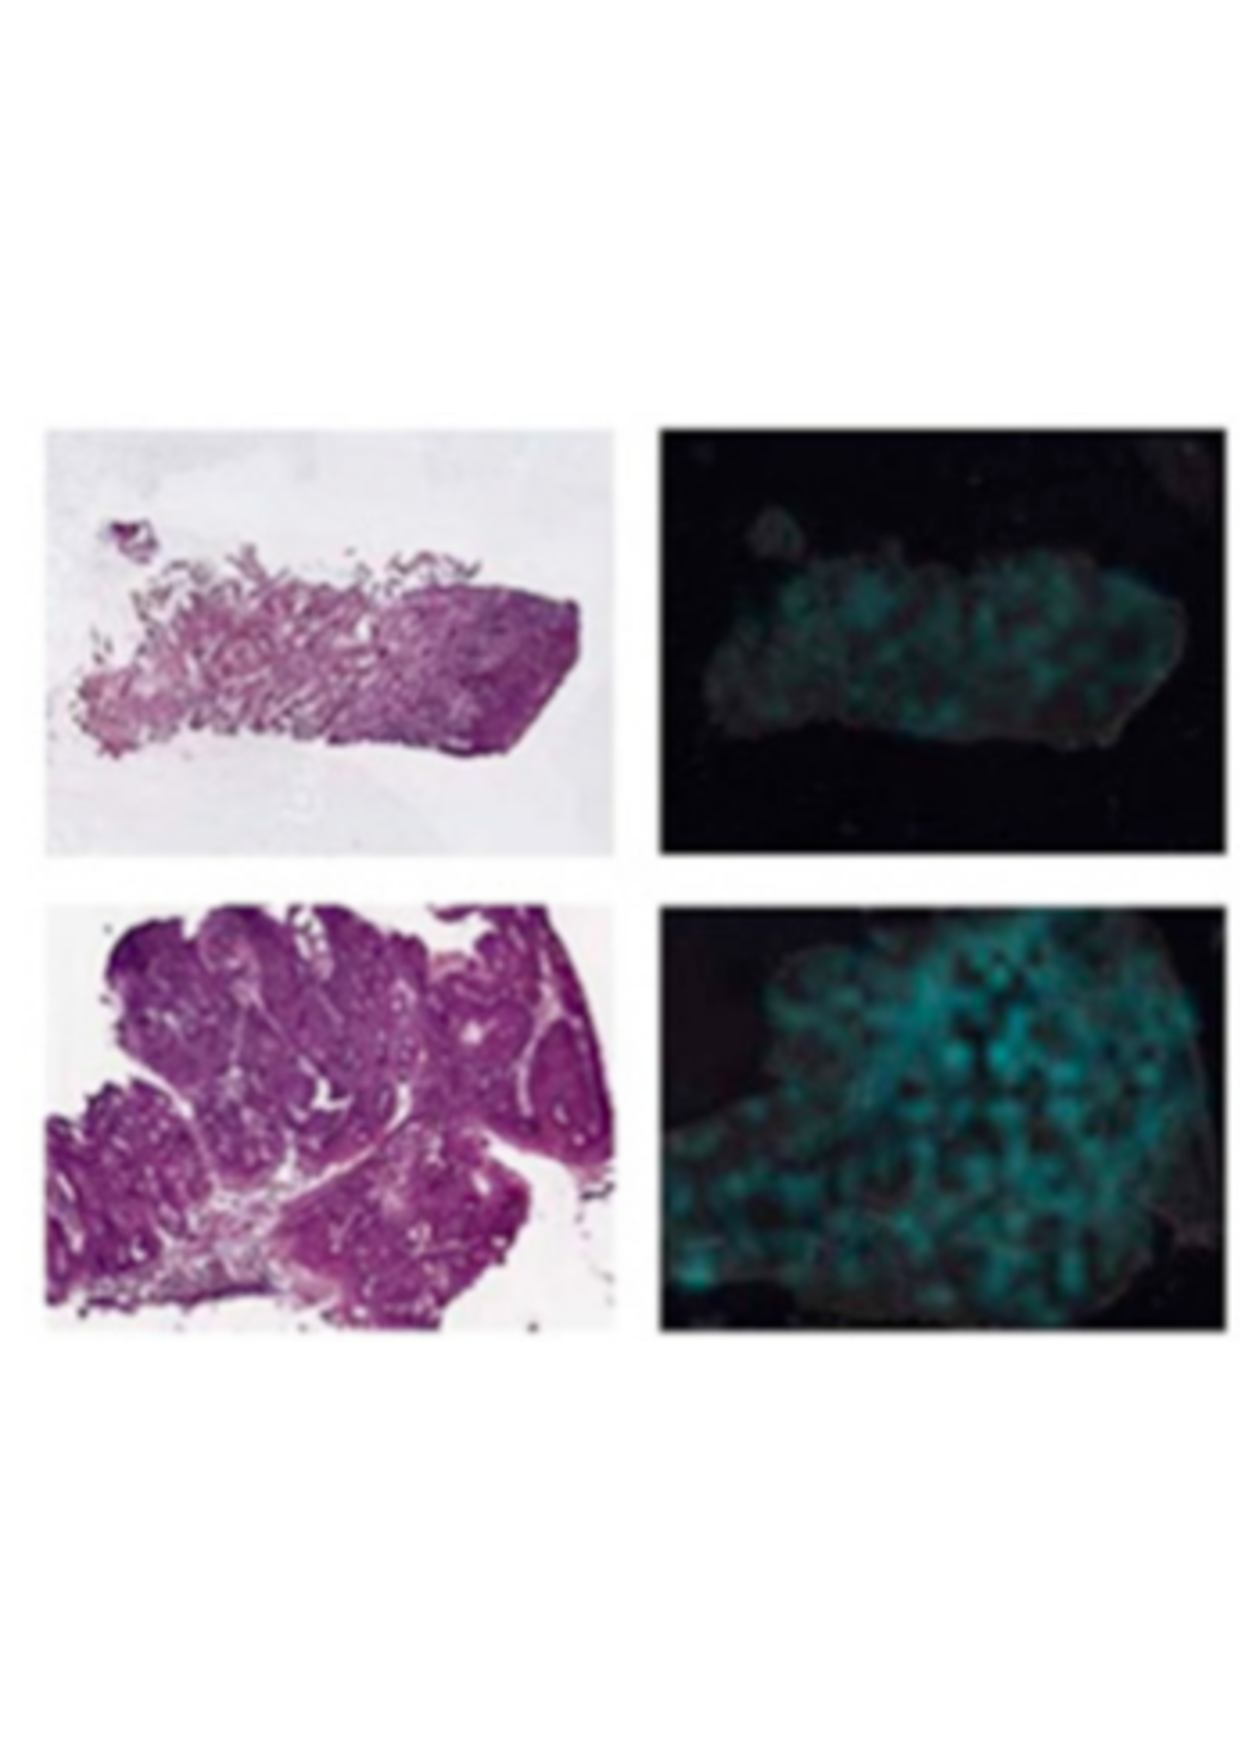
\includegraphics[width=4cm]{Figure_MALDI_spectra.pdf}\\
%\caption{
\small unknown protein at m/z 4968.1
\end{minipage}


\clearpage


%%
\subsection{LC-MS/MS for Cell Lines Analysis}
\thispagestyle{headings}
\markright{Statistics \hfill Protein library from HNSCC cell lines  \hfill}



\begin{outline} % for highlight
\1 \hl{cell lines}:
    \2 normal oral mucosa: OMF and NHOK 
    \2 HNSCC: Ca9-22, CAL-27, HSC-3, SAS, SCC-4, TW1.5, and TW2.6

\1 \hl{protein} of cell lysate
    \2 separated by molecular weight under 15\% SDS-polyacrylamide gel electrophoresis (SDS-PAGE)
    \2 in-gel \textcolor{red}{digestion} by trypsin enzyme (Promega)
\1 \hl{peptides} analysed by 
    \2 \acrshort{lcms} (i.e., LTQ/FT-ICR) {\tiny (liquid chromatography (\textcolor{red}{LC)}) $\longrightarrow$ linear ion trap quadrupole (\textcolor{red}{LTQ}) mass spectrometer $\longrightarrow$ Fourier transform-ion cyclotron resonance (\textcolor{red}{FT-ICR}) mass spectrometer, Thermo Electron)} % a kind of tandem mass spectrometer)}
%\1 a linear ion trap quadrupole (LTQ) tandem mass spectrometer (LTQ-FT LC-MS/MS, Thermo Electron)
    \2 \textcolor{red}{peptide mapping}: searching in protein database \tiny (IPI human, International Protein Index, compiled by the European Bioinformatics Institute)

%\1 A collection of $X_1...X_n$ features from cancer datasets
\end{outline}


%%%
\clearpage



\section{Results for (A)}

\clearpage


%%%%%%%%

% MALDI image
%% Figure-1_MALDI_Hsiao_B.PDF
% Figure-1_MALDI_Hsiao_D.PDF
\thispagestyle{headings}
\markright{Results\hfill Step 1: MALDI imaging \hfill}


\begin{figure}[ht]
%\subsubsection{Figure 2:h}
%\begin{figure}[H]
%    \captionsetup[subfigure]{
%  font=footnotesize,
%  justification=raggedright
%  skip=10pt
%    }
%    \setlength{\abovecaptionskip}{35pt plus 3pt minus 2pt} % Chosen fairly arbitrarily
%\centering
%\floatbox[{\capbeside\thisfloatsetup{capbesideposition={right,center},capbesidewidth=.35\linewidth,capbesidesep=quad}}]{figure}[\FBwidth]
%\centering
% not \widefigure
%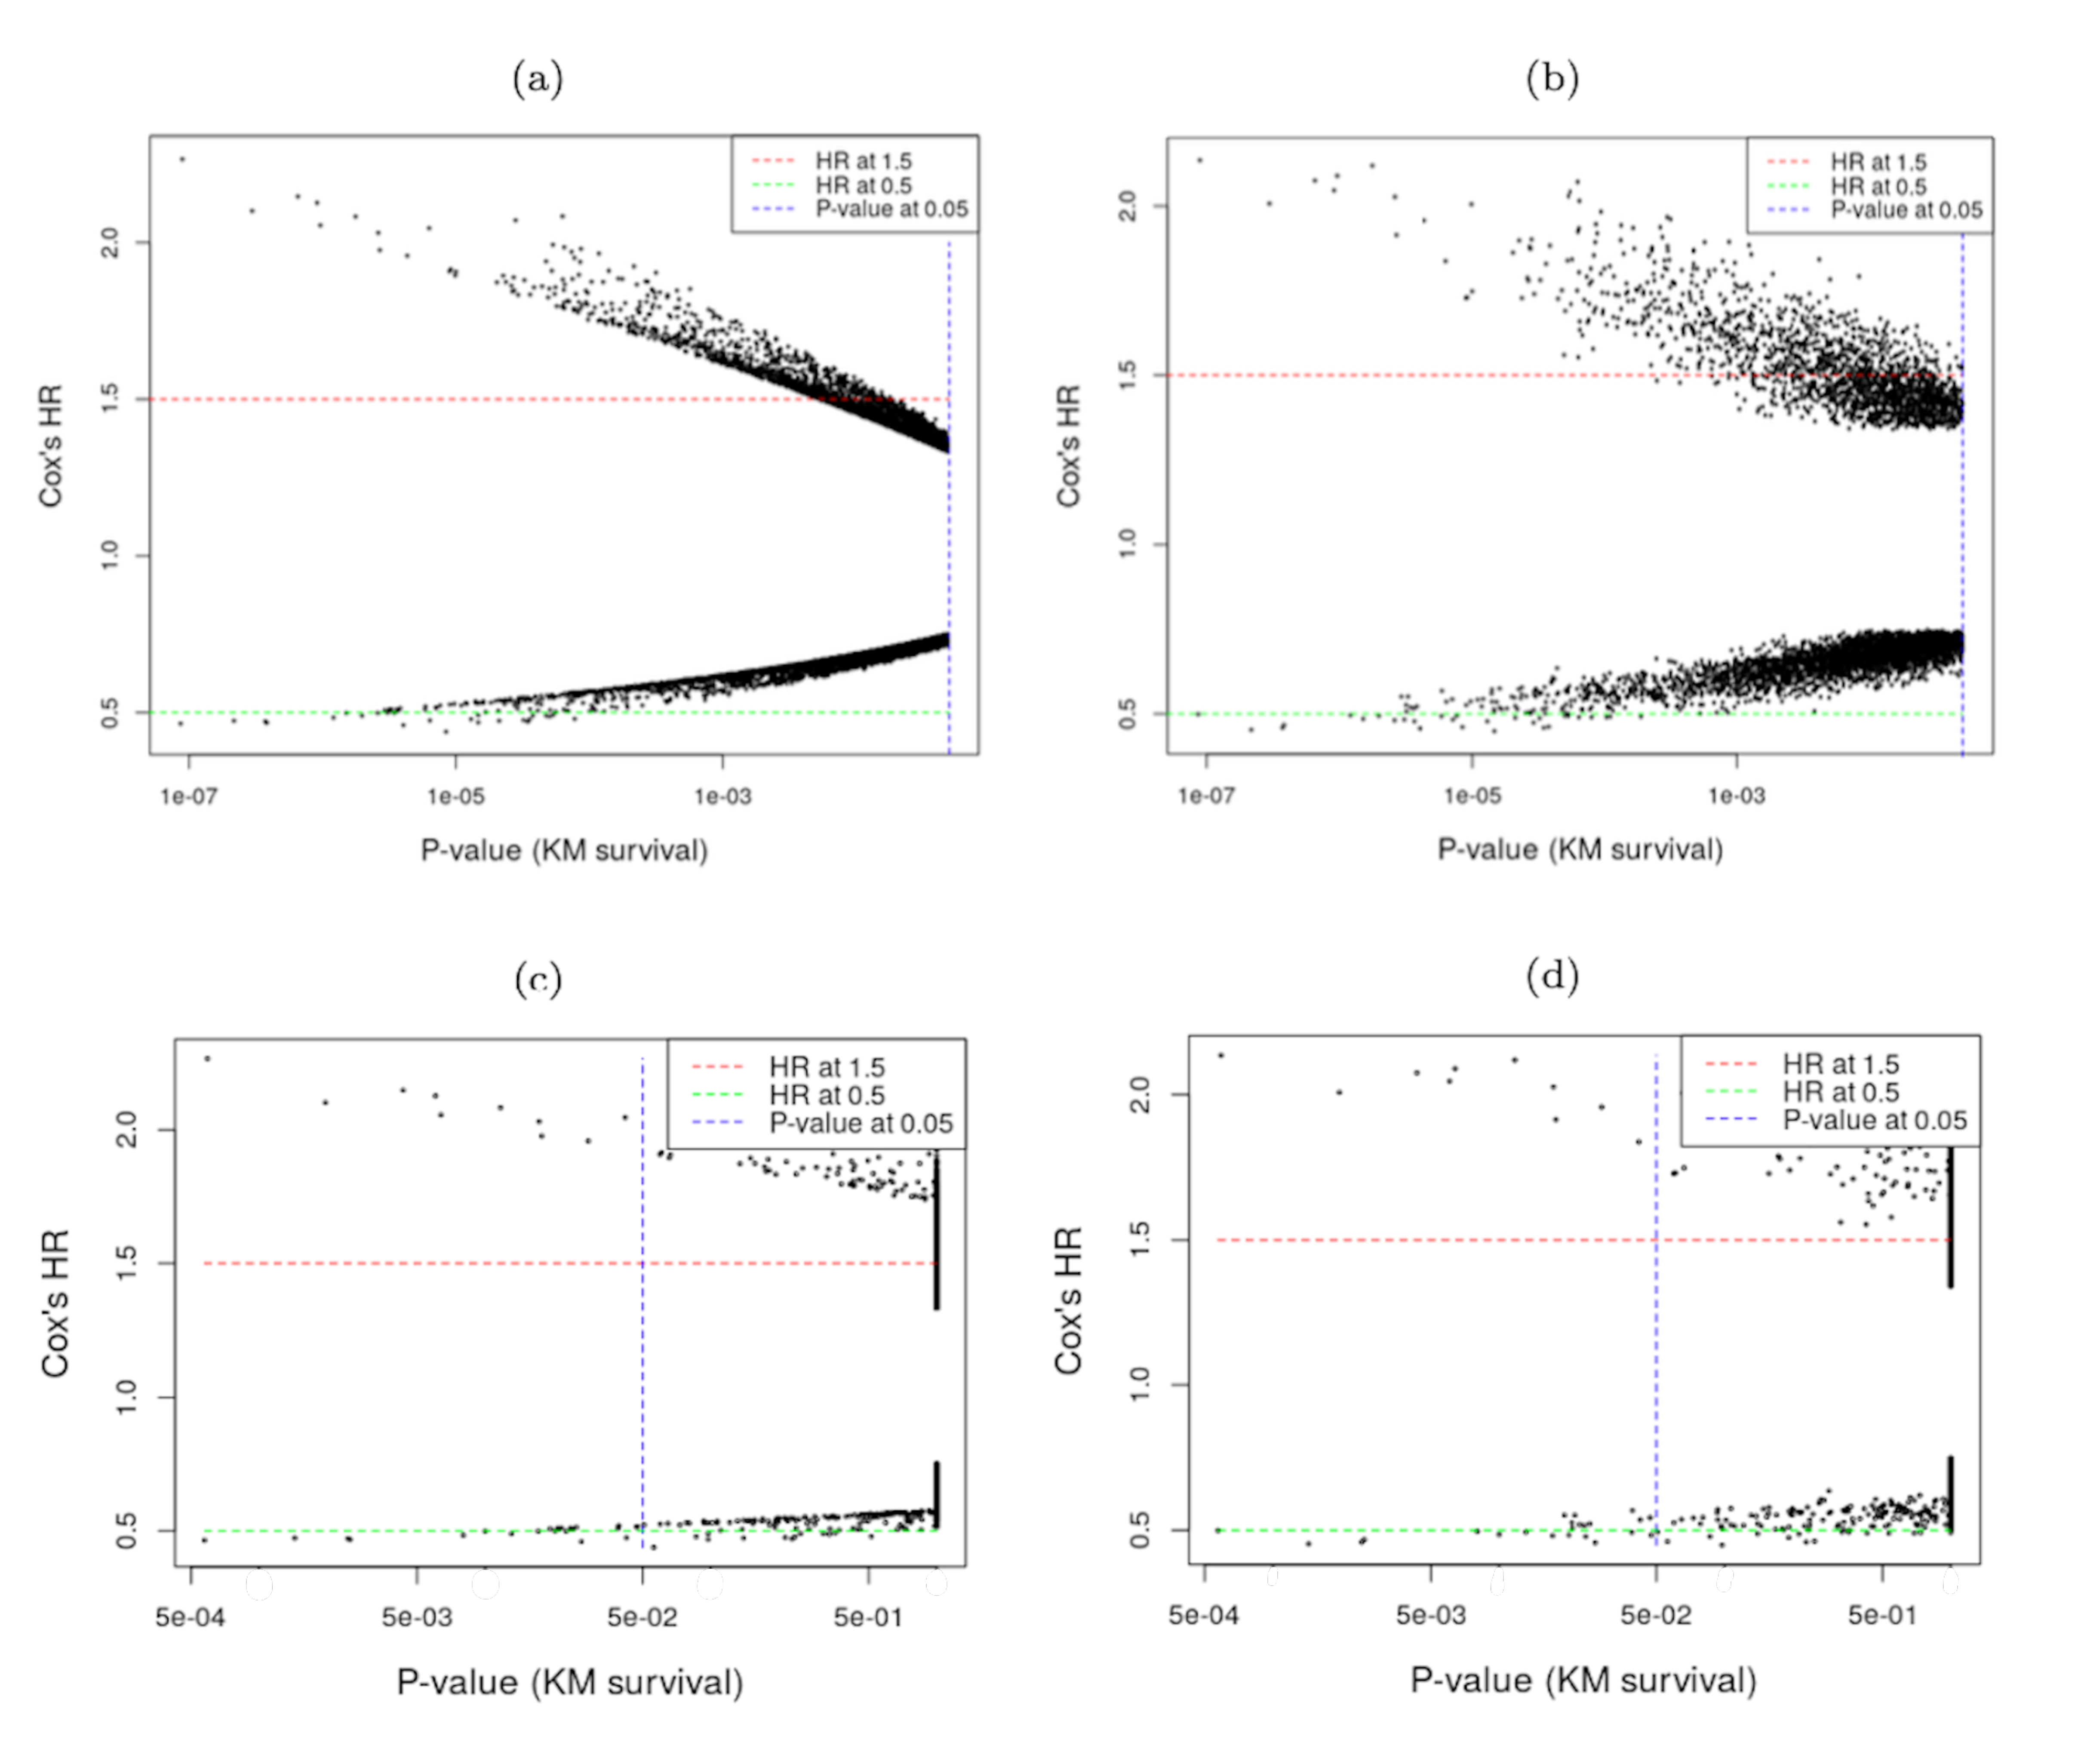
\includegraphics[width=14cm]{Figure2.pdf} %MDPI: Please revise the scientific notation format to a × 10b, and picture is not clear.ok
%\https://en.wikibooks.org/wiki/LaTeX/Floats,_Figures_and_Captions
% 2 by 2


%% ab
    \begin{subfigure}[t]{0.5\textwidth}
%\subfloat[Subfigure 1 list of figures text][(a)]{
%        \vspace*{-5mm}
%        \caption{~}
%        \fbox{
        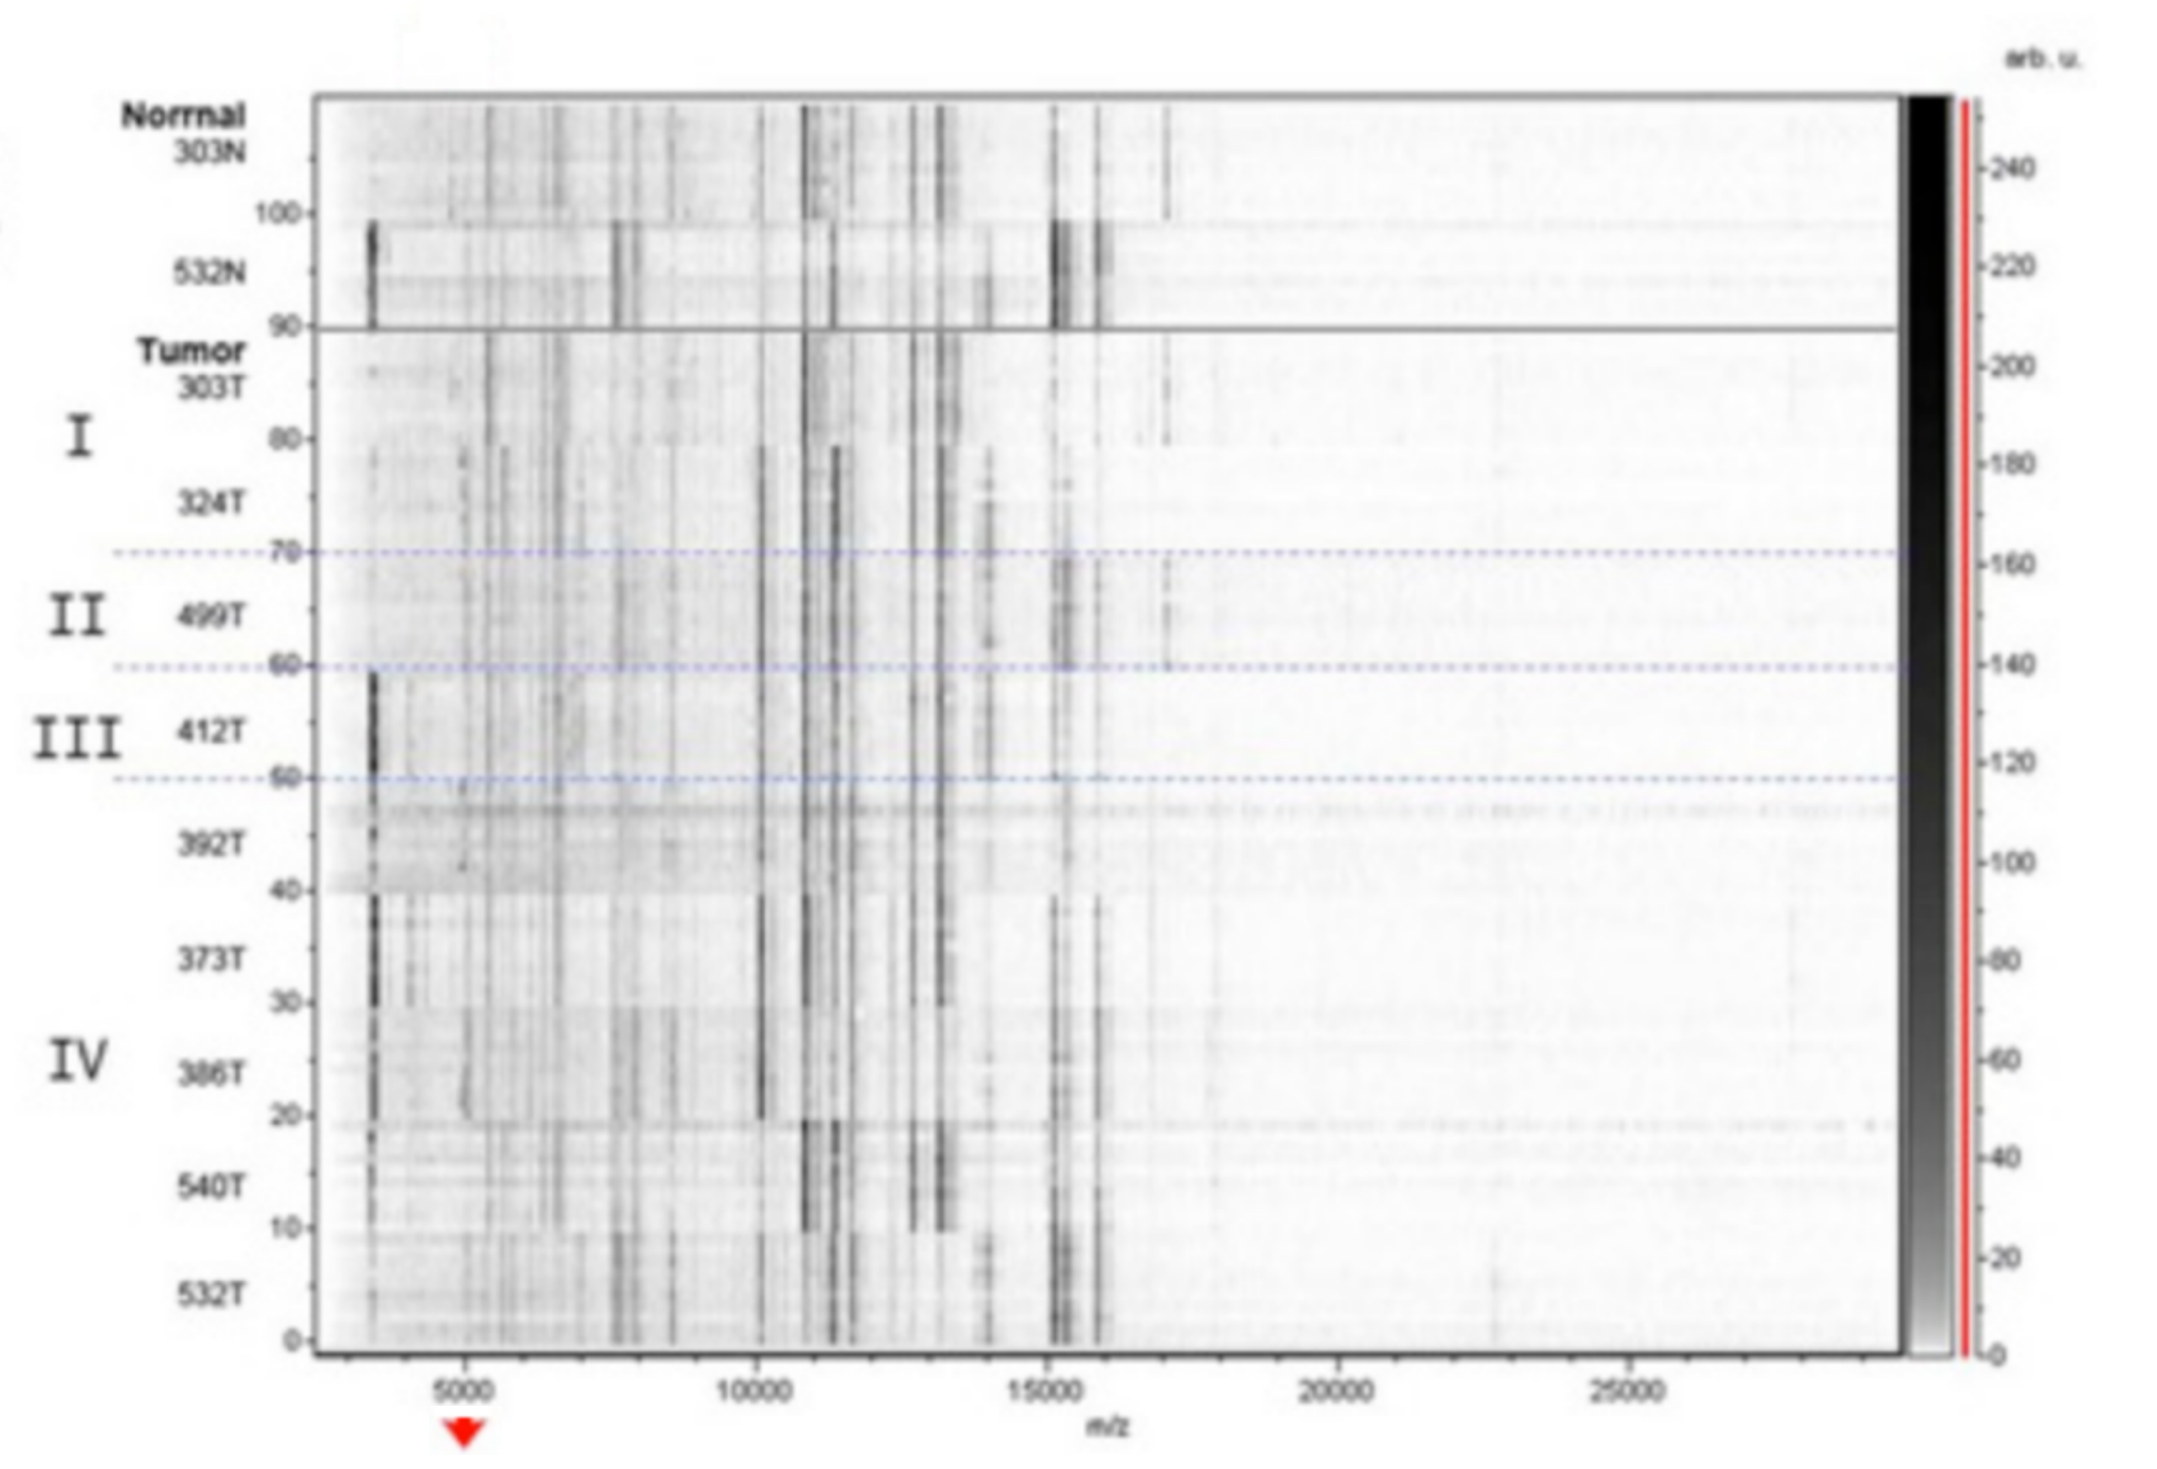
\includegraphics[width=6.5cm]{Figure-1_MALDI_Hsiao_B.PDF}  %}    %{Rplot02_rawP_uniHR.pdf}

    \end{subfigure} %\hfill
    \begin{subfigure}[t]{0.10\textwidth}
        \begin{picture}(0,0) % lower left corner
            \put(10,100){\large \textcolor{green}{Less}} \put(10,40){\large \textcolor{red}{More}}
        \end{picture}
    \end{subfigure}
%\subfloat[Subfigure 1 list of figures text][(b)]{
    \begin{subfigure}[t]{0.3\textwidth}
%        \caption{}
        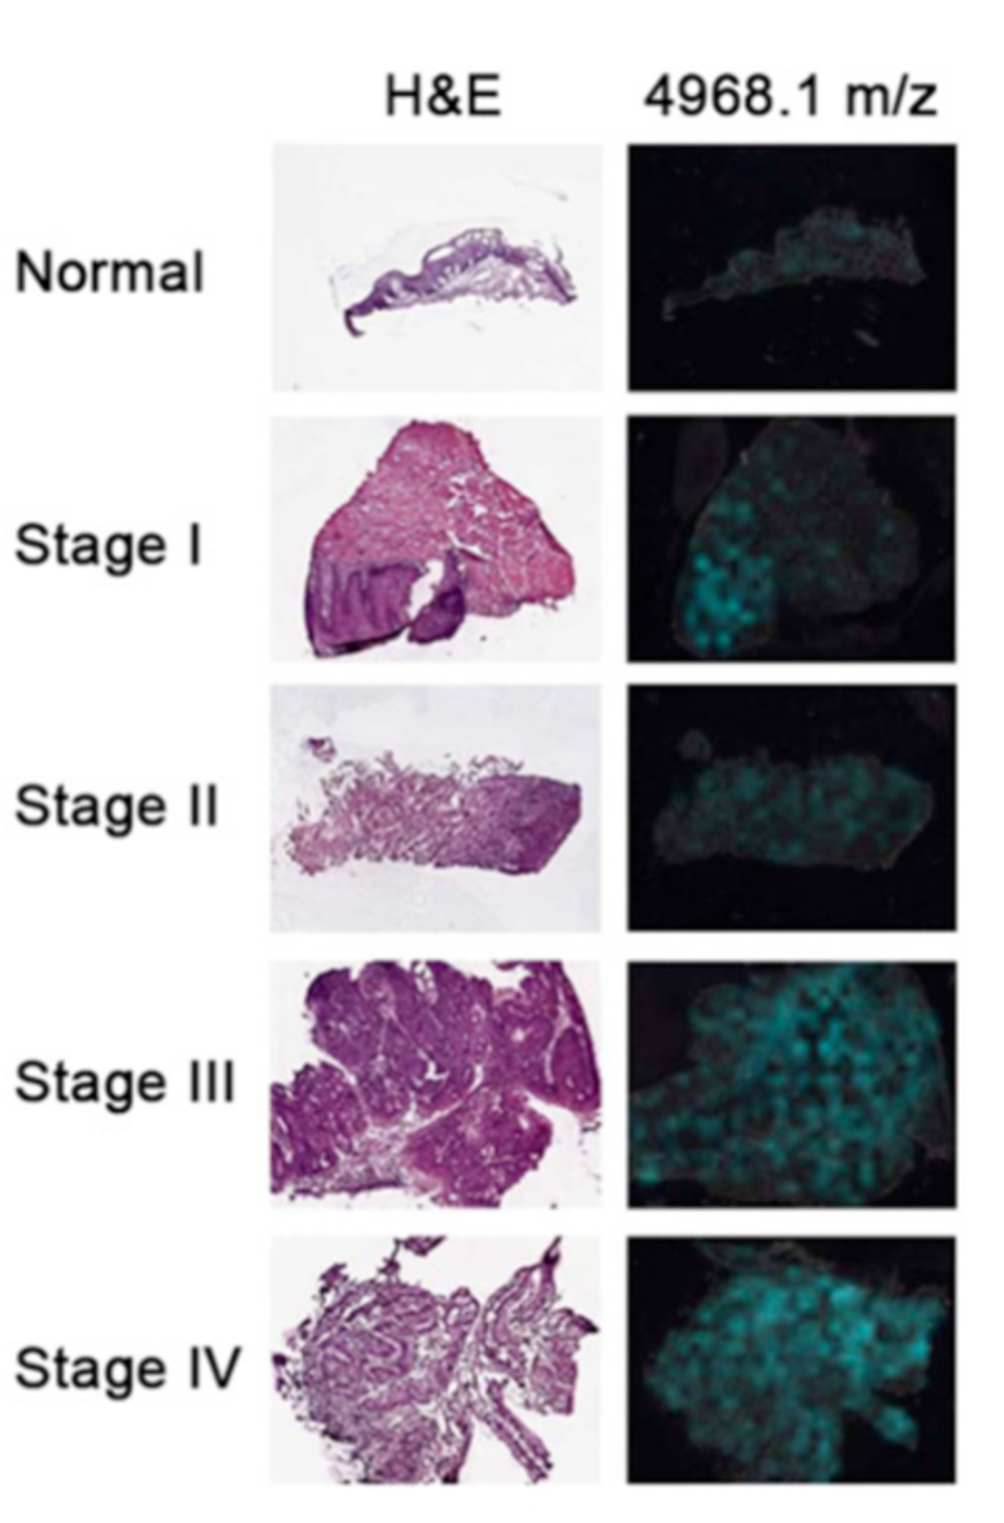
\includegraphics[height=6cm]{Figure-1_MALDI_Hsiao_D.PDF}
%        \caption{}
    \end{subfigure} \\
%\end{adjustwidth}
%    \vskip\baselineskip
% ,clip,keepaspectratio, ,height=6.5cm
%\vspace{0.3cm}

\captionsetup{labelformat=empty}
\caption{
\textcolor{red}{\hspace{15mm} (peak at m/z 5000) \hfill}\\
\vspace{5mm}
%A over-expressed protein, found by \acrshort{maldii} at \textcolor{red}{4968.1} m/z, is incrementally stronger by the stages. % of \acrshort{hnscc}.
An over-expressed protein at \textcolor{red}{m/z 4968.1}: (N)ormal $<$ (T)umor stage I $<$ II $<$ III $<$ IV
%\hl{FDR-adjusted} Kaplan--Meier (KM) estimate (\textit{p}~value (\textless{} 0.05; 9,416 genes)
}

\end{figure}

\clearpage
%%%%%%%%%%%%%%

%% top 10 MALDI table
\thispagestyle{headings}
\markright{Results\hfill The top 10 peak in MALDI Imaging  \hfill}

%\label{tab:Table1} 
\begin{longtable}{|r|r|r|r|r|r|r|}
%\caption[Peptides found by MALDI Imaging]{The top 10 peak expression ranked by T to N ratio in \acrshort{maldii} (Table courtesy of~\autocite{Chi2017})}\\ 
\hline
\rowcolor[rgb]{0.745,0.753,0.749} \multicolumn{1}{|c|}{Mass} & \multicolumn{1}{c|}{PTTA*} & \multicolumn{1}{c|}{N(mean)} & \multicolumn{1}{c|}{T(mean)} & \multicolumn{1}{c|}{N(SD)} & \multicolumn{1}{c|}{T(SD)} & 
\multicolumn{1}{|c|}{T/N}  \endfirsthead 
\hline
{\cellcolor[rgb]{0.863,0.863,0.863}}10099.8                  & \num{7.98E-16}                   & 341.9                        & 1509.6                       & 188.2                      & 1009.9                     & 4.4                       \\ 
\hline
{\cellcolor[rgb]{0.863,0.863,0.863}}10900.9                  & \num{3.64E-17}                   & 113.6                        & 425.3                        & 40.6                       & 253.0                      & 3.7                       \\ 
\hline
{\cellcolor[rgb]{0.863,0.863,0.863}}4048.6                   & \num{7.34E-13}                   & 18.4                         & 47.7                         & 3.5                        & 30.5                       & 2.6                       \\ 
\hline
{\cellcolor[rgb]{0.863,0.863,0.863}}11659.2                  & \num{1.17E-07}                   & 300.6                        & 733.7                        & 222.4                      & 321.3                      & 2.4                       \\ 
\hline
{\cellcolor[rgb]{0.863,0.863,0.863}}10306.9                  & \num{1.86E-15}                   & 104.2                        & 247.2                        & 34.7                       & 111.2                      & 2.4                       \\ 
\hline
{\cellcolor[rgb]{0.863,0.863,0.863}}9756.5                   & \num{2.75E-13}                   & 31.4                         & 71.6                         & 8.1                        & 38.8                       & 2.3                       \\ 
\hline
{\cellcolor[rgb]{0.863,0.863,0.863}}\textcolor{red}{4968.1}                   & \num{1.47E-02}                   & 28.0                         & 62.8                         & 14.0                       & 109.8                      & 2.2                       \\ 
\hline
{\cellcolor[rgb]{0.863,0.863,0.863}}11370.2                  & \num{3.94E-06}                   & 576.2                        & 1237.7                       & 362.1                      & 828.0                      & 2.1                       \\ 
\hline
{\cellcolor[rgb]{0.863,0.863,0.863}}11731.0                  & \num{1.83E-10}                   & 69.9                         & 150.2                        & 27.1                       & 78.6                       & 2.1                       \\ 
\hline
{\cellcolor[rgb]{0.863,0.863,0.863}}10532.3                  & \num{7.72E-16}                   & 48.4                         & 96.7                         & 11.6                       & 35.8                       & 2.0                       \\ 
\hline
\end{longtable}

{\tiny
*\acrshort{ptta}: the \acrlong{ptta} of the individual peak;
\acrshort{anova}: \acrlong{anova}.
N(mean): the average intensity in normal tissue;
%N(SD): the standard deviation of intensity in normal tissue;\\
T(mean): the average intensity in tumor specimen.
%T(SD): the standard deviation of intensity in tumor specimen;\\
%T/N: the ratio of T(mean)/N(mean).
}

\clearpage



%%%%%%%%%%%%%%


% next slide: LC-MS/MS Figure-1_MALDI_Hsiao_C.PDF
\thispagestyle{headings}
\markright{Results\hfill Step 2: LC-MS/MS for cell lines \hfill}

\begin{figure}
  \begin{minipage}[c]{0.35\linewidth}
  \begin{picture}(15, 20) % zero point at left end/H mid-line of (15,20) %(1,0.55038404)%
\centering
  \put(5,-65){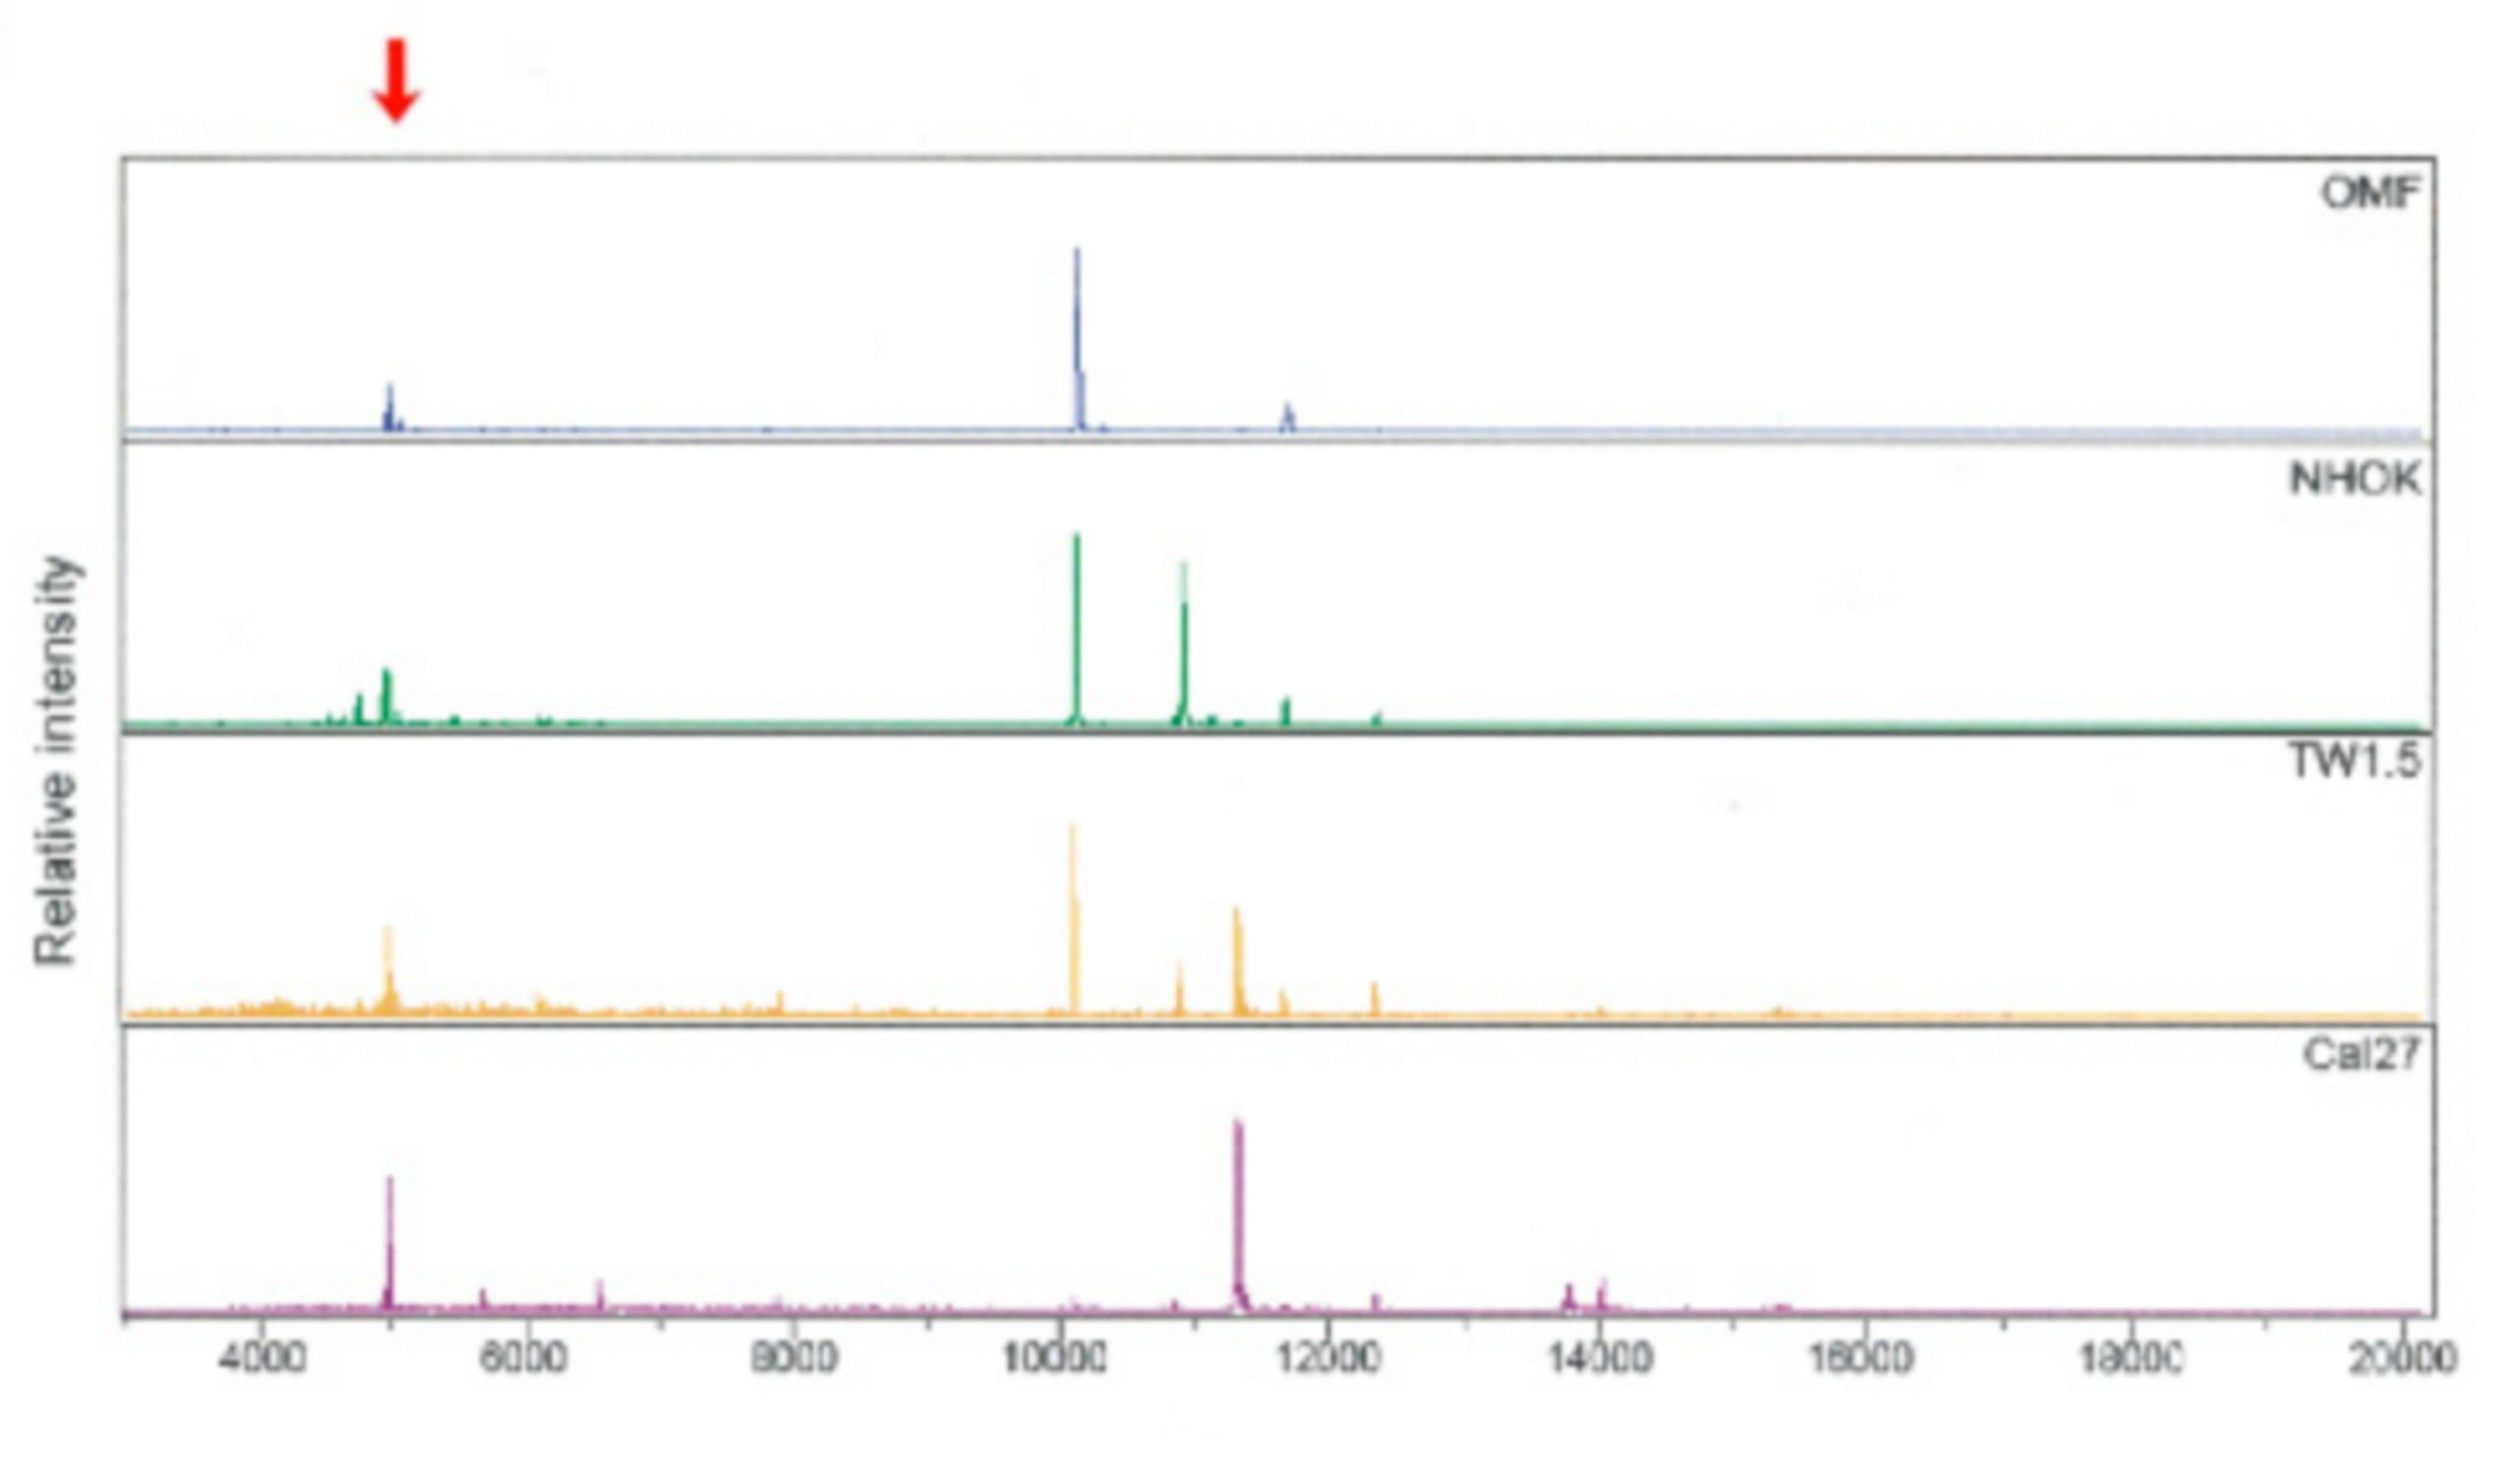
\includegraphics[width=7.0cm]{Figure-1_MALDI_Hsiao_C_Dalton.pdf}}
  %% Figure-1_MALDI_Hsiao_C.PDF}}
  %graphic_abstract_pvalueTex.pdf}}% X-axis: hyphen to minus sign
%    \includegraphics[height=7.0cm, width=7.5cm]{graphic_abstract_pvalueTex.pdf}%
    \captionsetup{labelformat=empty}
%    \caption{Figure. Mindfulness meditation in \hl{holistic} cancer care}
  \put(25.5, 53.5){%\fontfamily{qcr}\selectfont
  \large  5000 Dalton} % 5053 Dalton protein: TMSB4X
  
  \put(112.5, 17){%\fontfamily{qcr}\selectfont
  \large Normal cells}
  
  \put(112.5, -30){%\fontfamily{qcr}\selectfont
  \large Tumor cells}
  
%  \put(2,-105){Figure. Overview of the strategy used for identification of the biomarker in \acrshort{hnscc}}
  %Mindfulness meditation in \hl{holistic} cancer care}
  
  \end{picture}
  \end{minipage}\hfill
  \begin{minipage}[c]{0.55\linewidth}
    \centering
    \begin{outline}[enumerate]
    \1 Peptide mapping for protein identification
%        \2 in-gel digestion, then
%        \2 analysis by linear ion trap quadrupole--Fourier transform \acrlong{lcms} (LTQ-FT \acrshort{lcms}, Thermo Electron) % tandem mass spectrometer
%    \1 Abundant protein found in normal oral cell lines (N: OMF and NHOK) and \acrshort{hnscc} cells (T: TW1.5 and CAL-27)
    %; \textcolor{red}{Red arrow} also indicates 
    \1 At the molecular weight around 5000 Dalton, the intensity is (N)ormal $<$ (T)umor.


    \end{outline}
%    \captionof{table} % by KOMA-script
%      {%
%        Different kinds of ducks%
%        \label{tab:duck}%
 %     }
  \end{minipage}
\end{figure}




\clearpage
%%%%%%%%%%%%%%

% find 4968.1 with IPI
% Figure-2_LC_cells_Hsiao2.PDF
\thispagestyle{headings}
\markright{Results\hfill Protein library in cell lines \hfill}

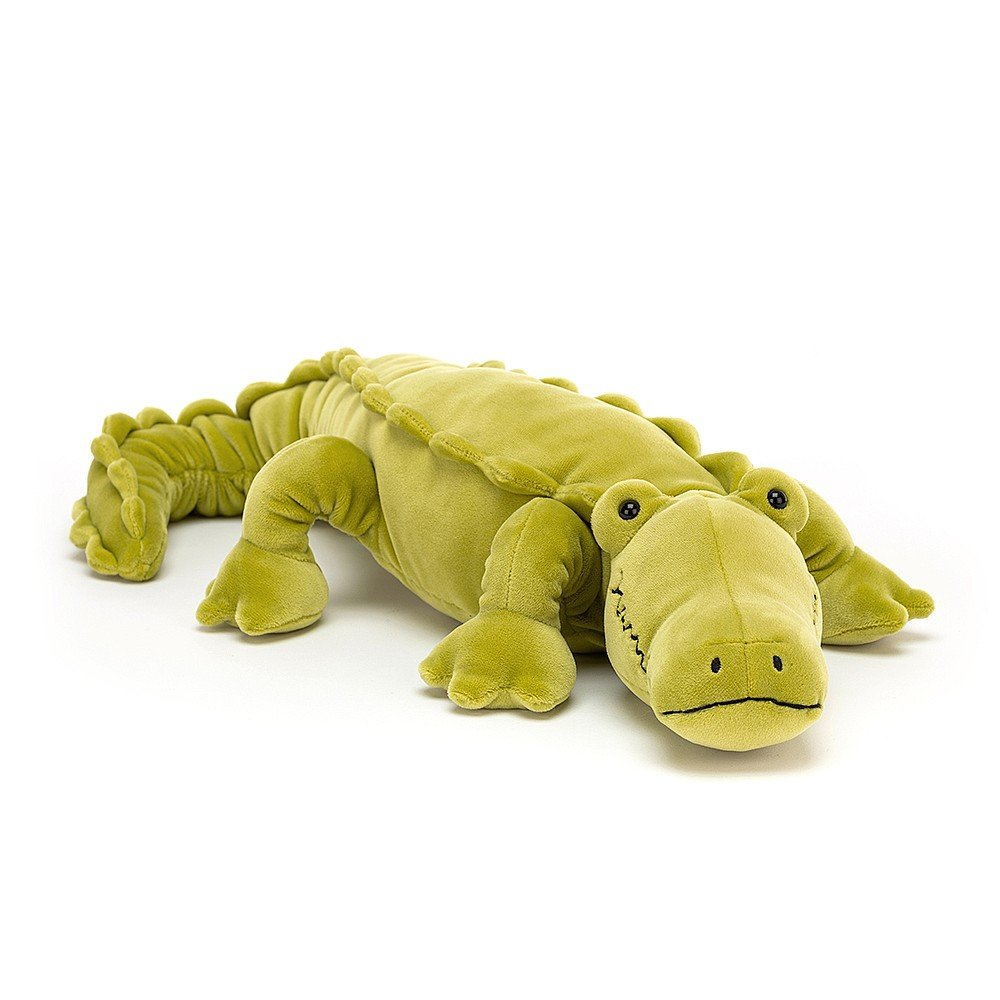
\includegraphics[width=5cm]{ZIG2C.jpg}
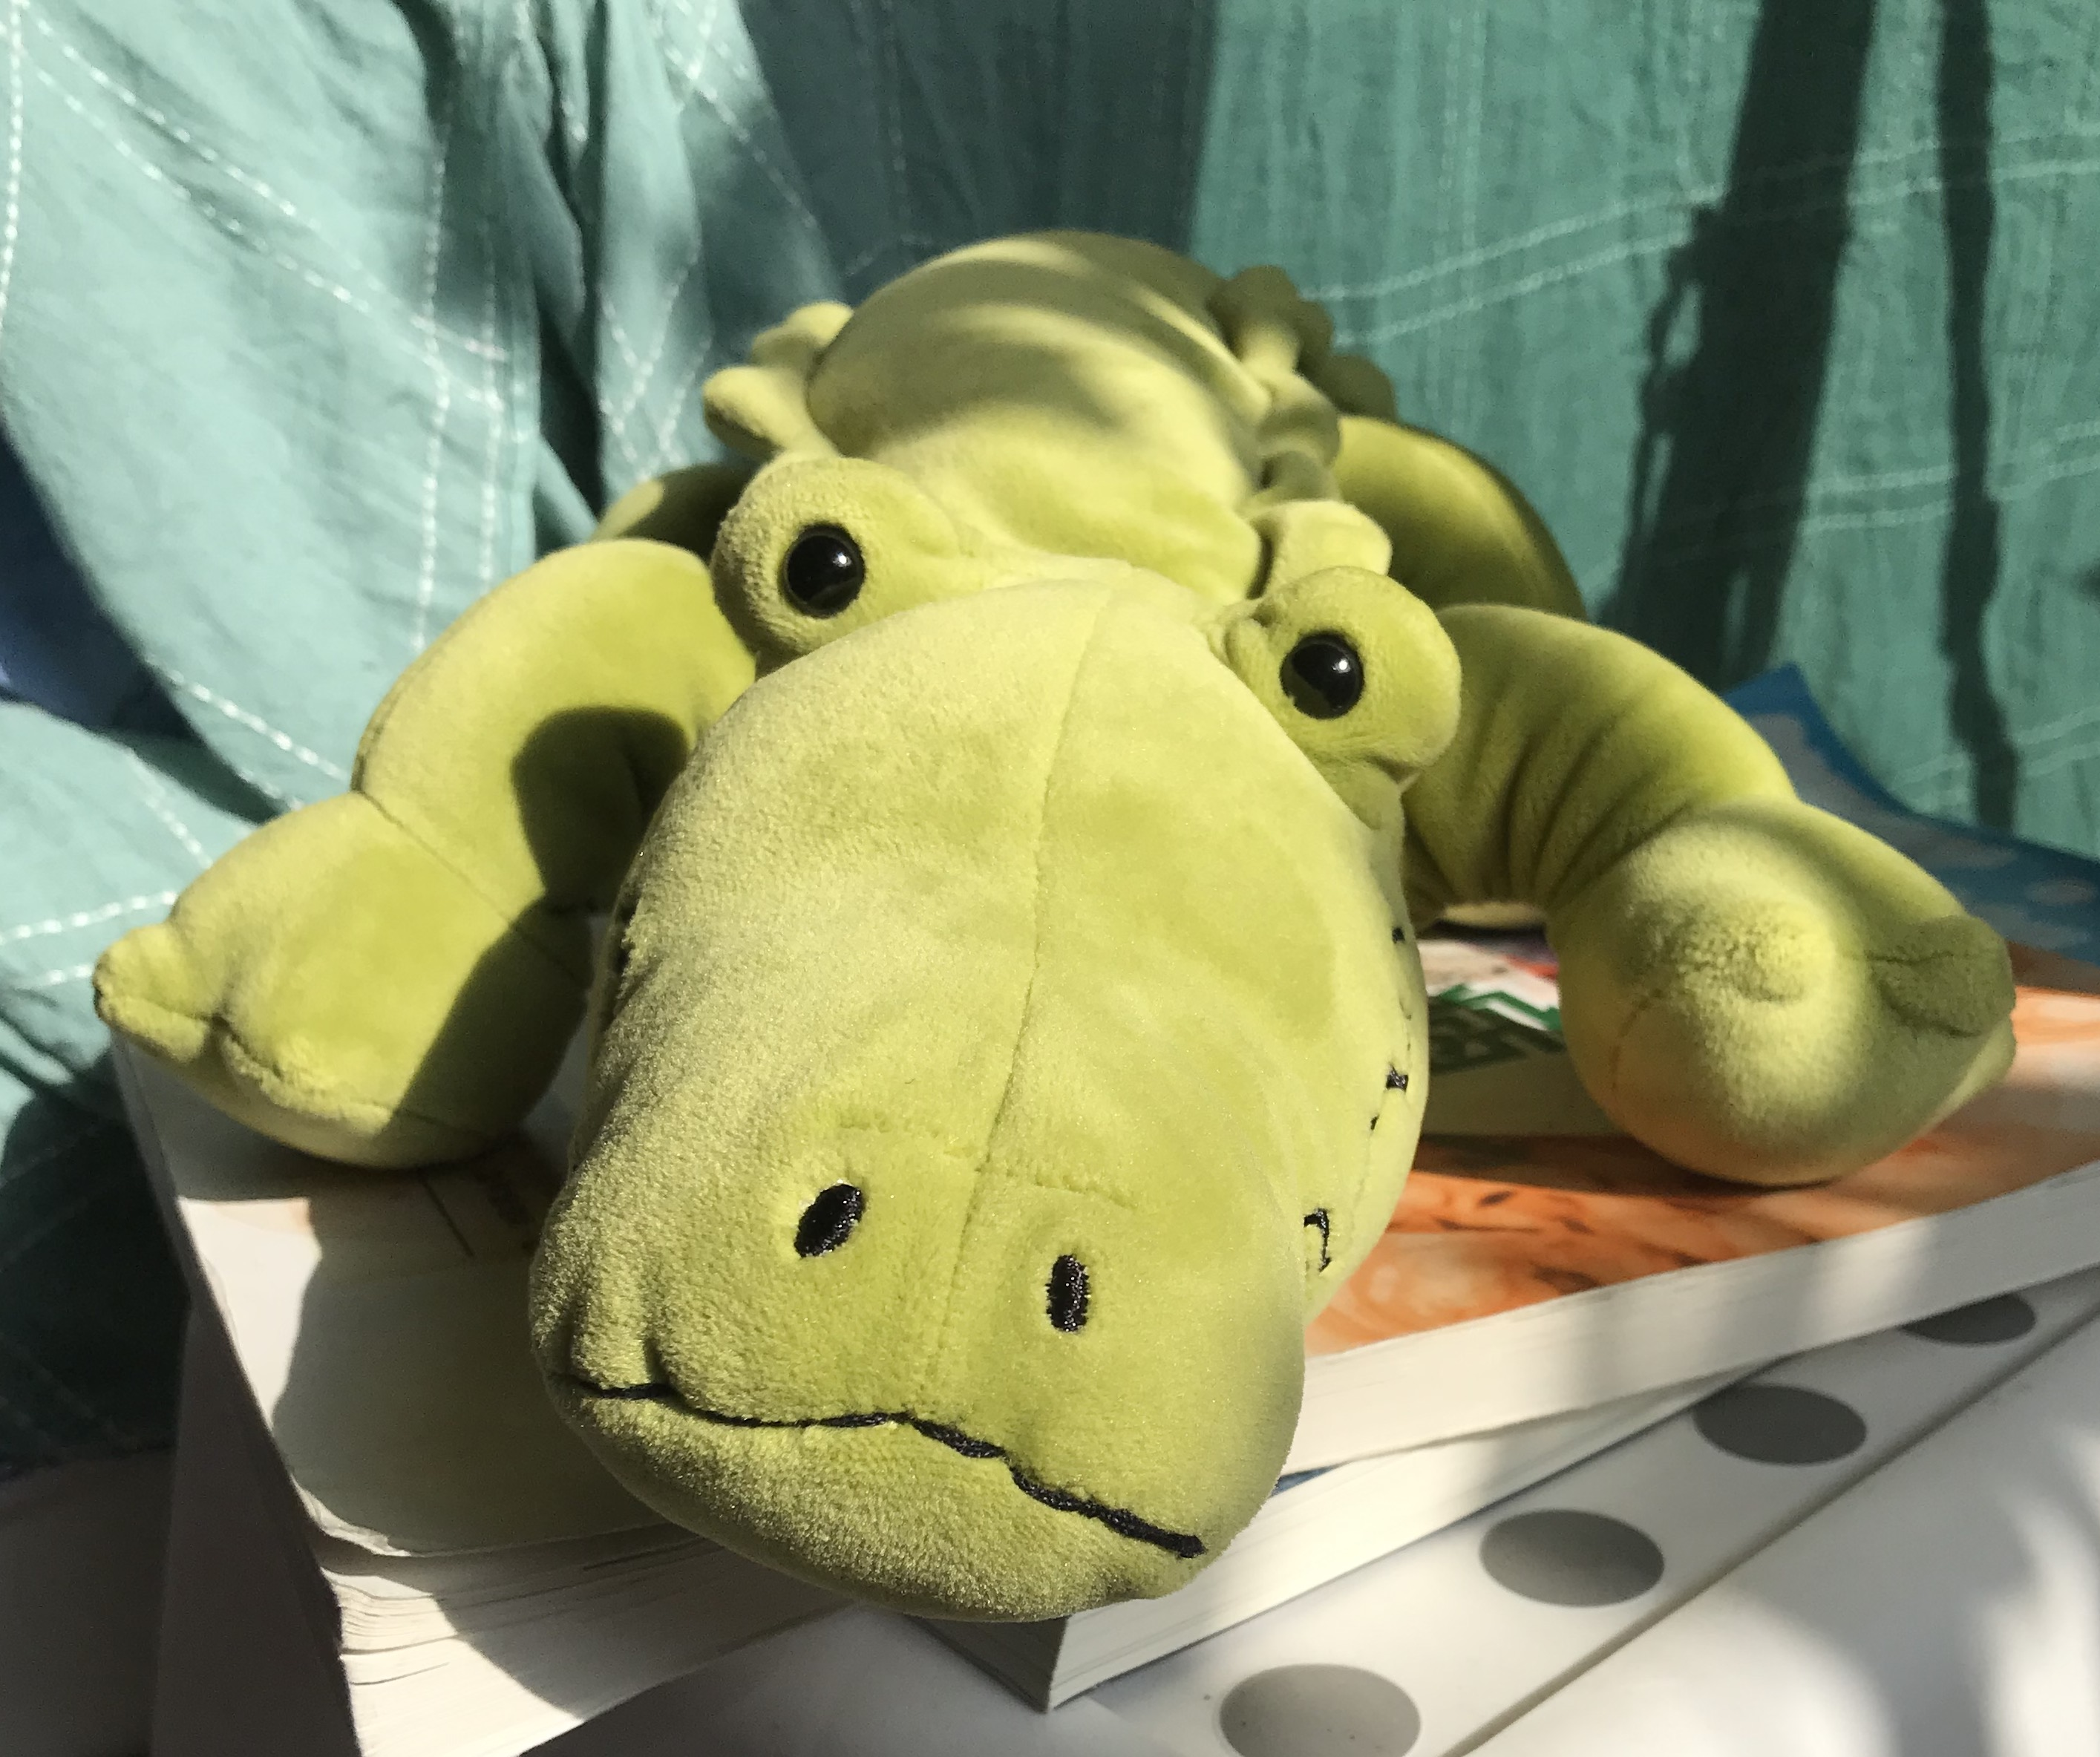
\includegraphics[width=3.5cm]{IMG_8273.jpg}
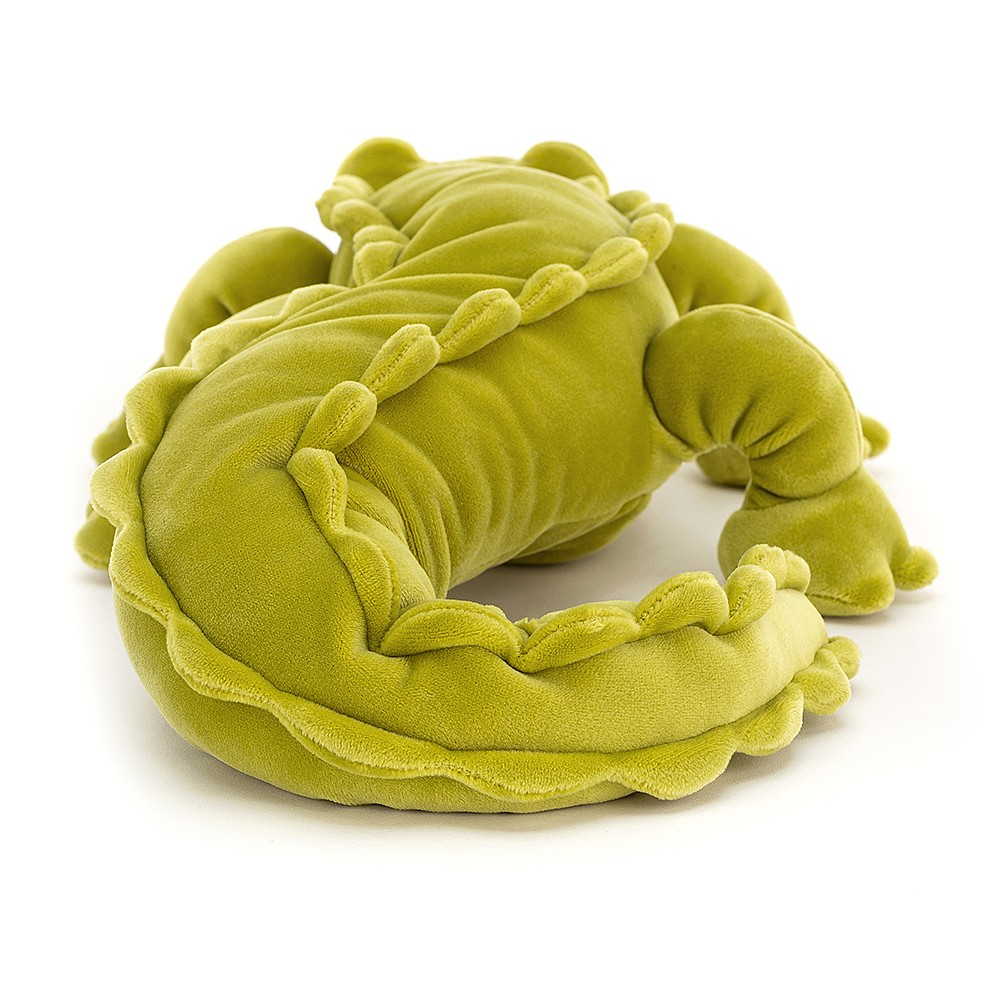
\includegraphics[width=4cm]{ZIG2C_2.jpg}
\\

{\tiny \hspace{4.5cm} Our team mascot: zigzag crocodile (jELLYCAT~\textsuperscript{TM})}\\
A Mascot search engine of peptide mapping for protein identification\\


\clearpage
%%%%%%%%%%%%%%%%%%%%%%


\thispagestyle{headings}
\markright{Results\hfill Protein library in cell lines  \hfill}

\begin{figure}[ht]

\floatbox[{\capbeside\thisfloatsetup{capbesideposition={right,center},capbesidewidth=.35\linewidth,capbesidesep=quad}}]{figure}[\FBwidth]
    %\centering
{    \includegraphics[width=9cm]{
Rplot_Figure_venn_163.eps
%Rplot_TCGA_HNSCC_CoxHR_CAMK2N1_top3FDRKM.pdf
}
}
{\captionsetup{labelformat=empty}    % Summary of identified proteins (venn diagram)]
\caption{
- Proteins {\scriptsize (by \acrshort{lcms})} of the cell lines of NHOK, OMF and \acrshort{hnscc}s. \\[0.2cm]
- \textcolor{red}{163 protein identities} are unique in TW1.5 and TW2.6 HNSCC cancer cells \\[0.2CM]
%- IPI00220828 (TMSB4X) is on the list of 163 proteins \\[0.5cm]
%    \textcolor{red}{Red spots}: HR > 1.0;\\
%    \textcolor{green}{Green spots}: HR < 1.0;\\
%    \textcolor{red}{Red dash line}: FDR \textit{p} = 0.05.\\
\tiny (OMF: oral mucosal fibroblast; NHOK: normal human oral keratinocyte)% TW1.5 and TW2.6: two cell lines of HNSCC)
    }}
%%%\label{fig:hazards3}
\end{figure}


%
\clearpage





%%
\begin{figure}
  \begin{minipage}[c]{0.35\linewidth}
  \begin{picture}(15, 20) % zero point at left end/H mid-line of (15,20) %(1,0.55038404)%
\centering
  \put(5,-65){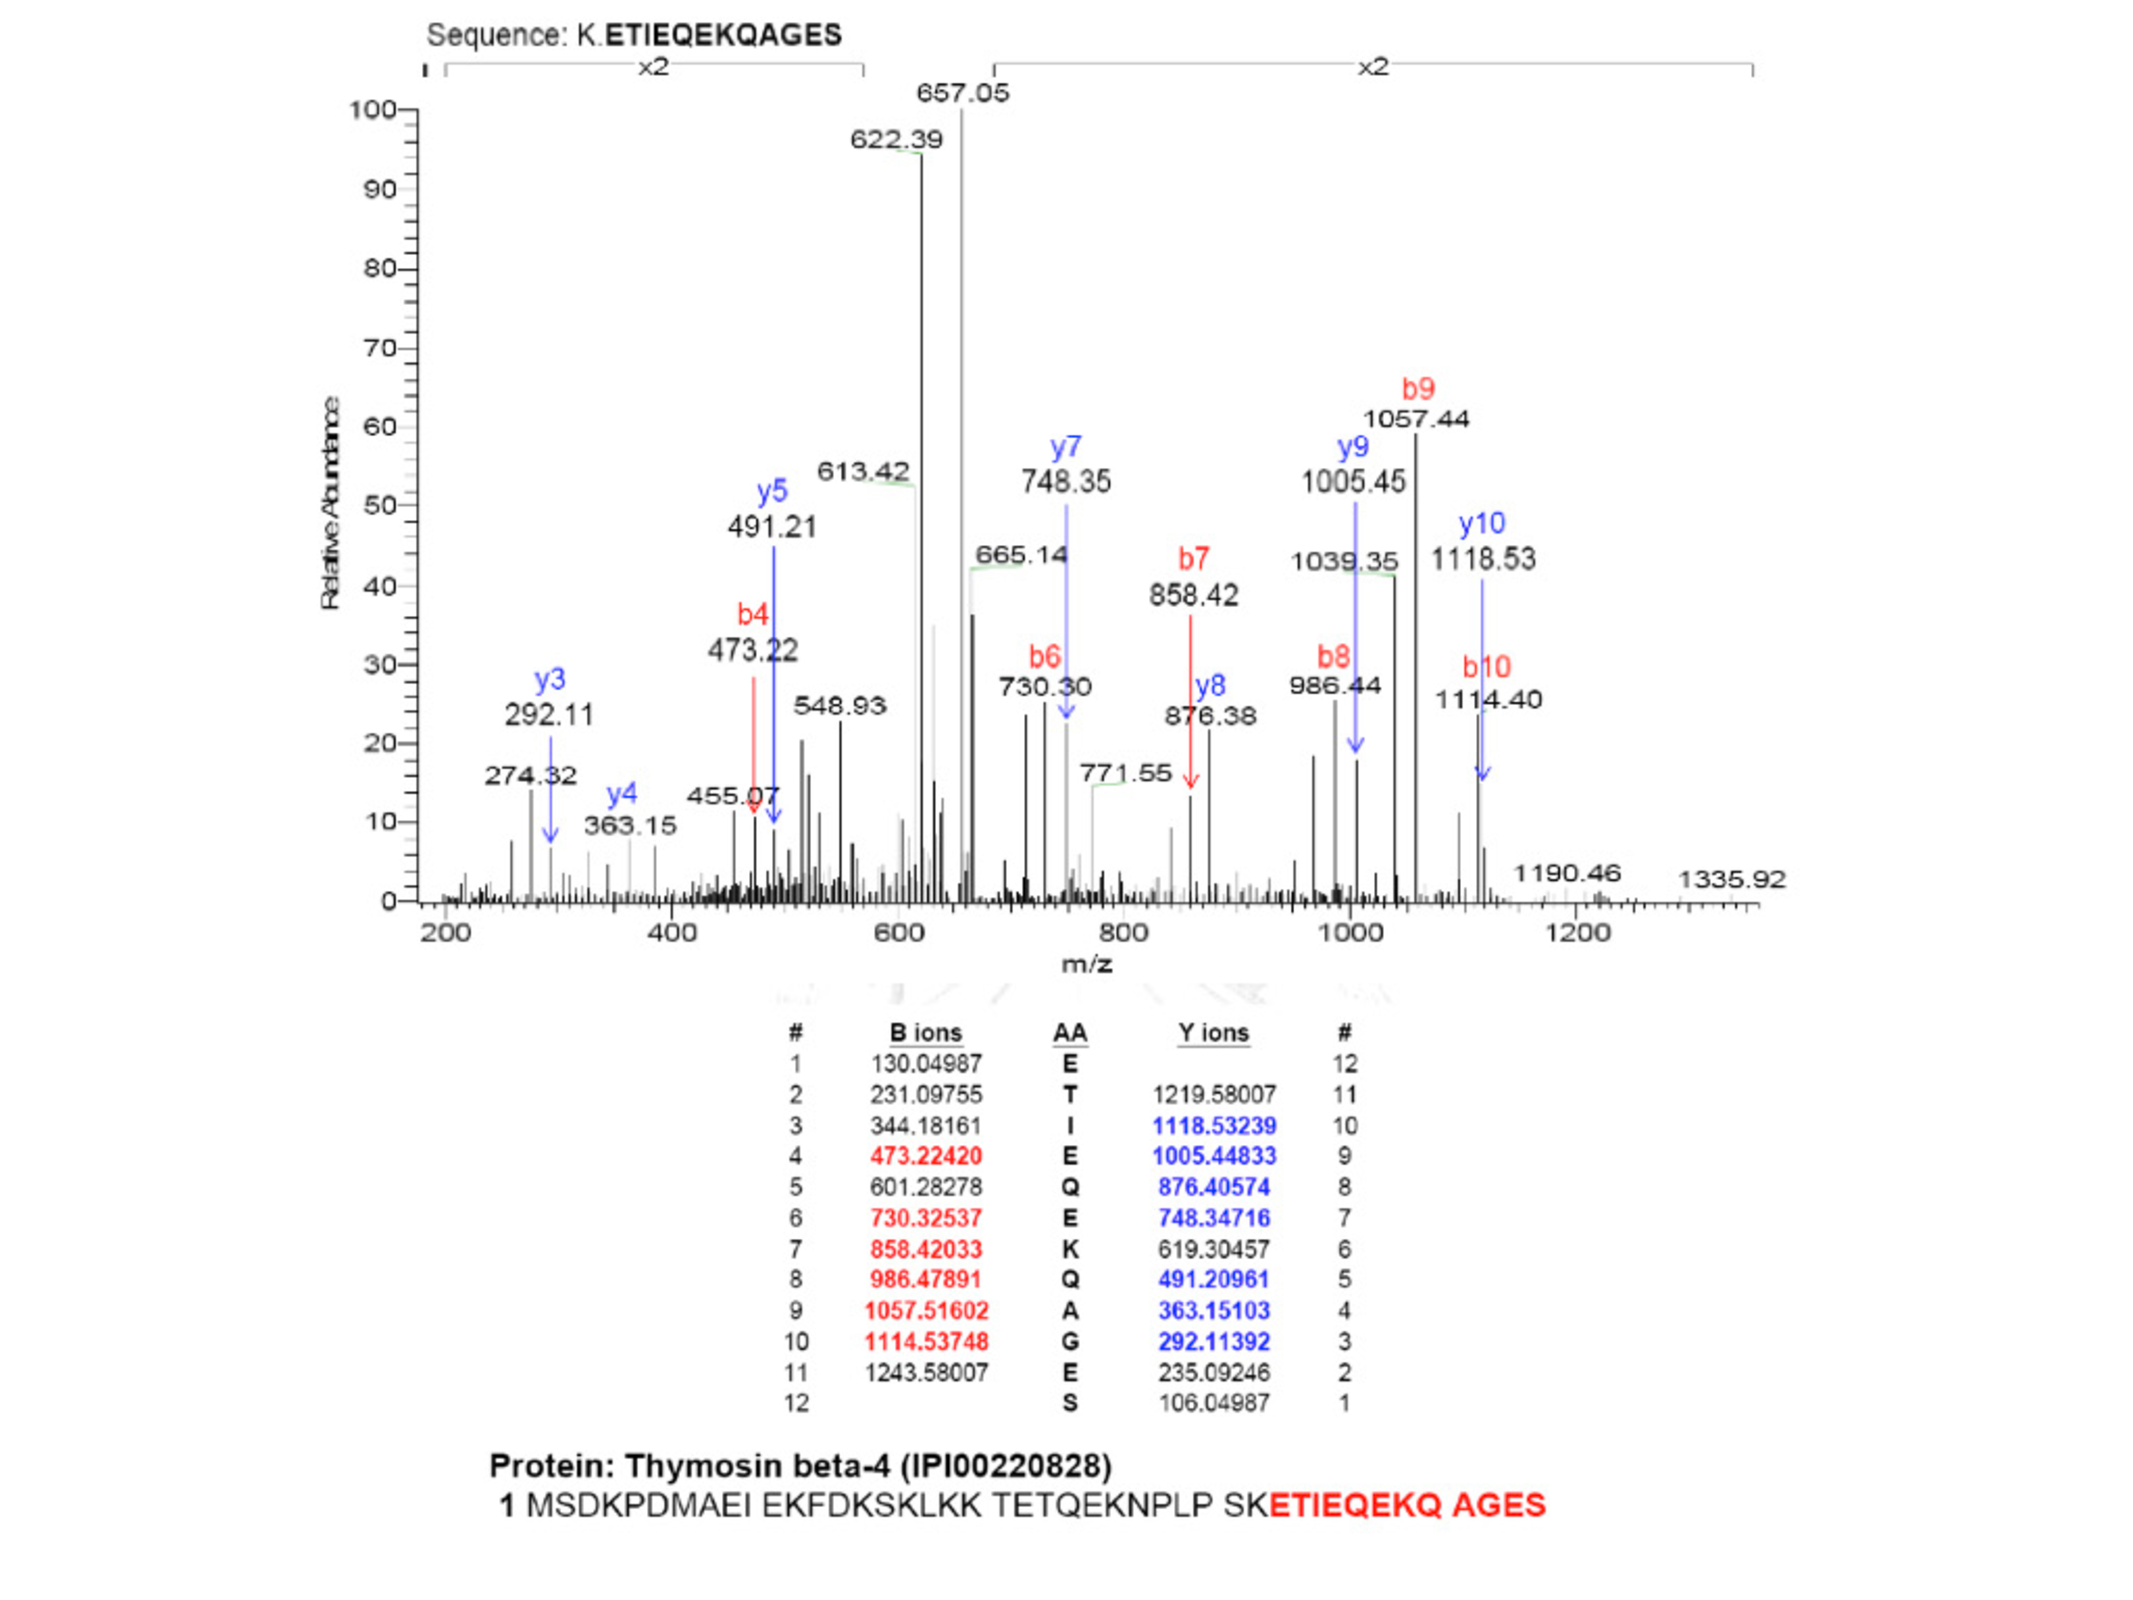
\includegraphics[width=8.5cm]{Figure-2_LC_cells_Hsiao2.PDF}}
  %graphic_abstract_pvalueTex.pdf}}% X-axis: hyphen to minus sign
%    \includegraphics[height=7.0cm, width=7.5cm]{graphic_abstract_pvalueTex.pdf}%
    \captionsetup{labelformat=empty}
%    \caption{Figure. Mindfulness meditation in \hl{holistic} cancer care}
%  \put(25.5, 53.5){%\fontfamily{qcr}\selectfont
%  \large  5000 m/z}
  
%  \put(112.5, 17){%\fontfamily{qcr}\selectfont
%  \large normal cells}
  
%  \put(112.5, -30){%\fontfamily{qcr}\selectfont
%  \large cancer cells}
  
%  \put(2,-105){Figure. Overview of the strategy used for identification of the biomarker in \acrshort{hnscc}}
  %Mindfulness meditation in \hl{holistic} cancer care}
  
  \end{picture}
  \end{minipage}\hfill
  \begin{minipage}[c]{0.45\linewidth}
    \centering
    \begin{outline}[enumerate]

\1 Mascot Search of peptide mapping (163 protein identities)
\1 TOF/TOF spectra with the \hl{amino acid sequencing} of peptide
\1 K.\textcolor{red}{ETIEQKQAGES} was identified in \acrshort{tmsb4x} (\hl{5053} Dalton)
%Peptide sequencing was indicated by matching \textcolor{red}{b}-ions and \textcolor{blue}{y}-ions fragments.

{\tiny The N-terminal charged fragment ions are classed as a, \textcolor{red}{b} or c, while the C-terminal charged ones are classed as x, \textcolor{blue}{y} or z) \\(Figure courtesy of~\autocite{Tai2007,Chi2017}) }
% http://www.matrixscience.com/help/fragmentation_help.html
    \end{outline}
%    \captionof{table} % by KOMA-script
%      {%
%        Different kinds of ducks%
%        \label{tab:duck}%
 %     }
  \end{minipage}
\end{figure}




\clearpage
%%%%%%%%%%%%%%%


%%%%%%%%%%%%%%%

\markright{Results \hfill   A biomarker candidate: TMSB4X \hfill}
\subsection{Identification and Validation}
our biomarker candidate: \acrfull{tmsb4x}

in vitro and in vivo experiments

\clearpage



%%%%%%%%%%%%%%%%%%




%%%%%%%%%%

\thispagestyle{headings}
\markright{Results \hfill TMSB4X expression in HNSCC:  N < T \hfill}

\begin{figure}[ht]

\floatbox[{\capbeside\thisfloatsetup{capbesideposition={right,center},capbesidewidth=.45\linewidth,capbesidesep=quad}}]{figure}[\FBwidth]
% TCGA FDR Pvalue of CAMK2N1 (1.628308e-05), IL19 ( 6.543871e-06), FCGBP (4.827833e-05), CALML5 (0.0001970348)
{\setlength{\unitlength}{.78cm}
\begin{picture}(10.5, 10) % (9,10) %(1,0.55038404)%
\centering
  \put(0,0){\includegraphics[height=7.5cm]{Figure-3_NT_Hsiao.pdf}}%
%  \put(1.3, 7.25){\fontfamily{qcr}\selectfont
%  \tiny *\protect\textit{p} = \num{1.63e-05}}%CAMK2N1
\put(1.3, 0){\fontfamily{qcr}\selectfont
 \tiny Score}
\put(3.0, 0){\fontfamily{qcr}\selectfont
 1}
\put(5.0, 0){\fontfamily{qcr}\selectfont
 3}
%\begin{annotationimage}{width=15cm}{Figure_4_CAMK2N1_IL19_FCGBP.pdf}
%\includegraphics[width=15cm]{Figure_4_CAMK2N1_IL19.pdf}
%\draw[annotation left = {Aries at 0.3}]

%\end{annotationimage}
\end{picture}%
}
%\hfill
{\captionsetup{labelformat=empty}
\caption{\textcolor{red}{N < T} \\[0.1cm]
\acrshort{tmsb4x} expression of \acrshort{hnscc} cohorts,\\[0.2cm] %normal surrounding tissues (N) < tumors (T):
\hl{in RNA level}\\
(A) and (B) 35 NT-paired samples of KVGH cohort;\\
% by \acrshort{rtpcr} and \acrshort{qpcr}, respectively. 
(C) 23 NT-paired microarray dataset, GSE31056 (\acrshort{tmsb4x} probe: 216438\_s\_at);\\[0.2cm]
\hl{in Protein level}\\
(D) The \acrfull{ihc} staining of tissue microarray in 31 NT-paired samples (out of n=86, TMUH cohort);\\
%scored as 0 or 3 
(E) \textcolor{red}{IHC score} = the intensity (i.e., 0 to 3) $\times$ the percentage (i.e., 0 to 100\%)\\
\tiny (* \protect\textit{p} values is estimated by paired t-test)
}}
%%%\label{fig:figure4}
\end{figure}

\clearpage

%%%%%%%%%%

\thispagestyle{headings}
\markright{Results\hfill TMSB4X has impact on HNSCC's prognosis \hfill}

\begin{figure}[ht]
\floatbox[{\capbeside\thisfloatsetup{capbesideposition={right,center},capbesidewidth=.35\linewidth,capbesidesep=quad}}]{figure}[\FBwidth]
   % \centering
{    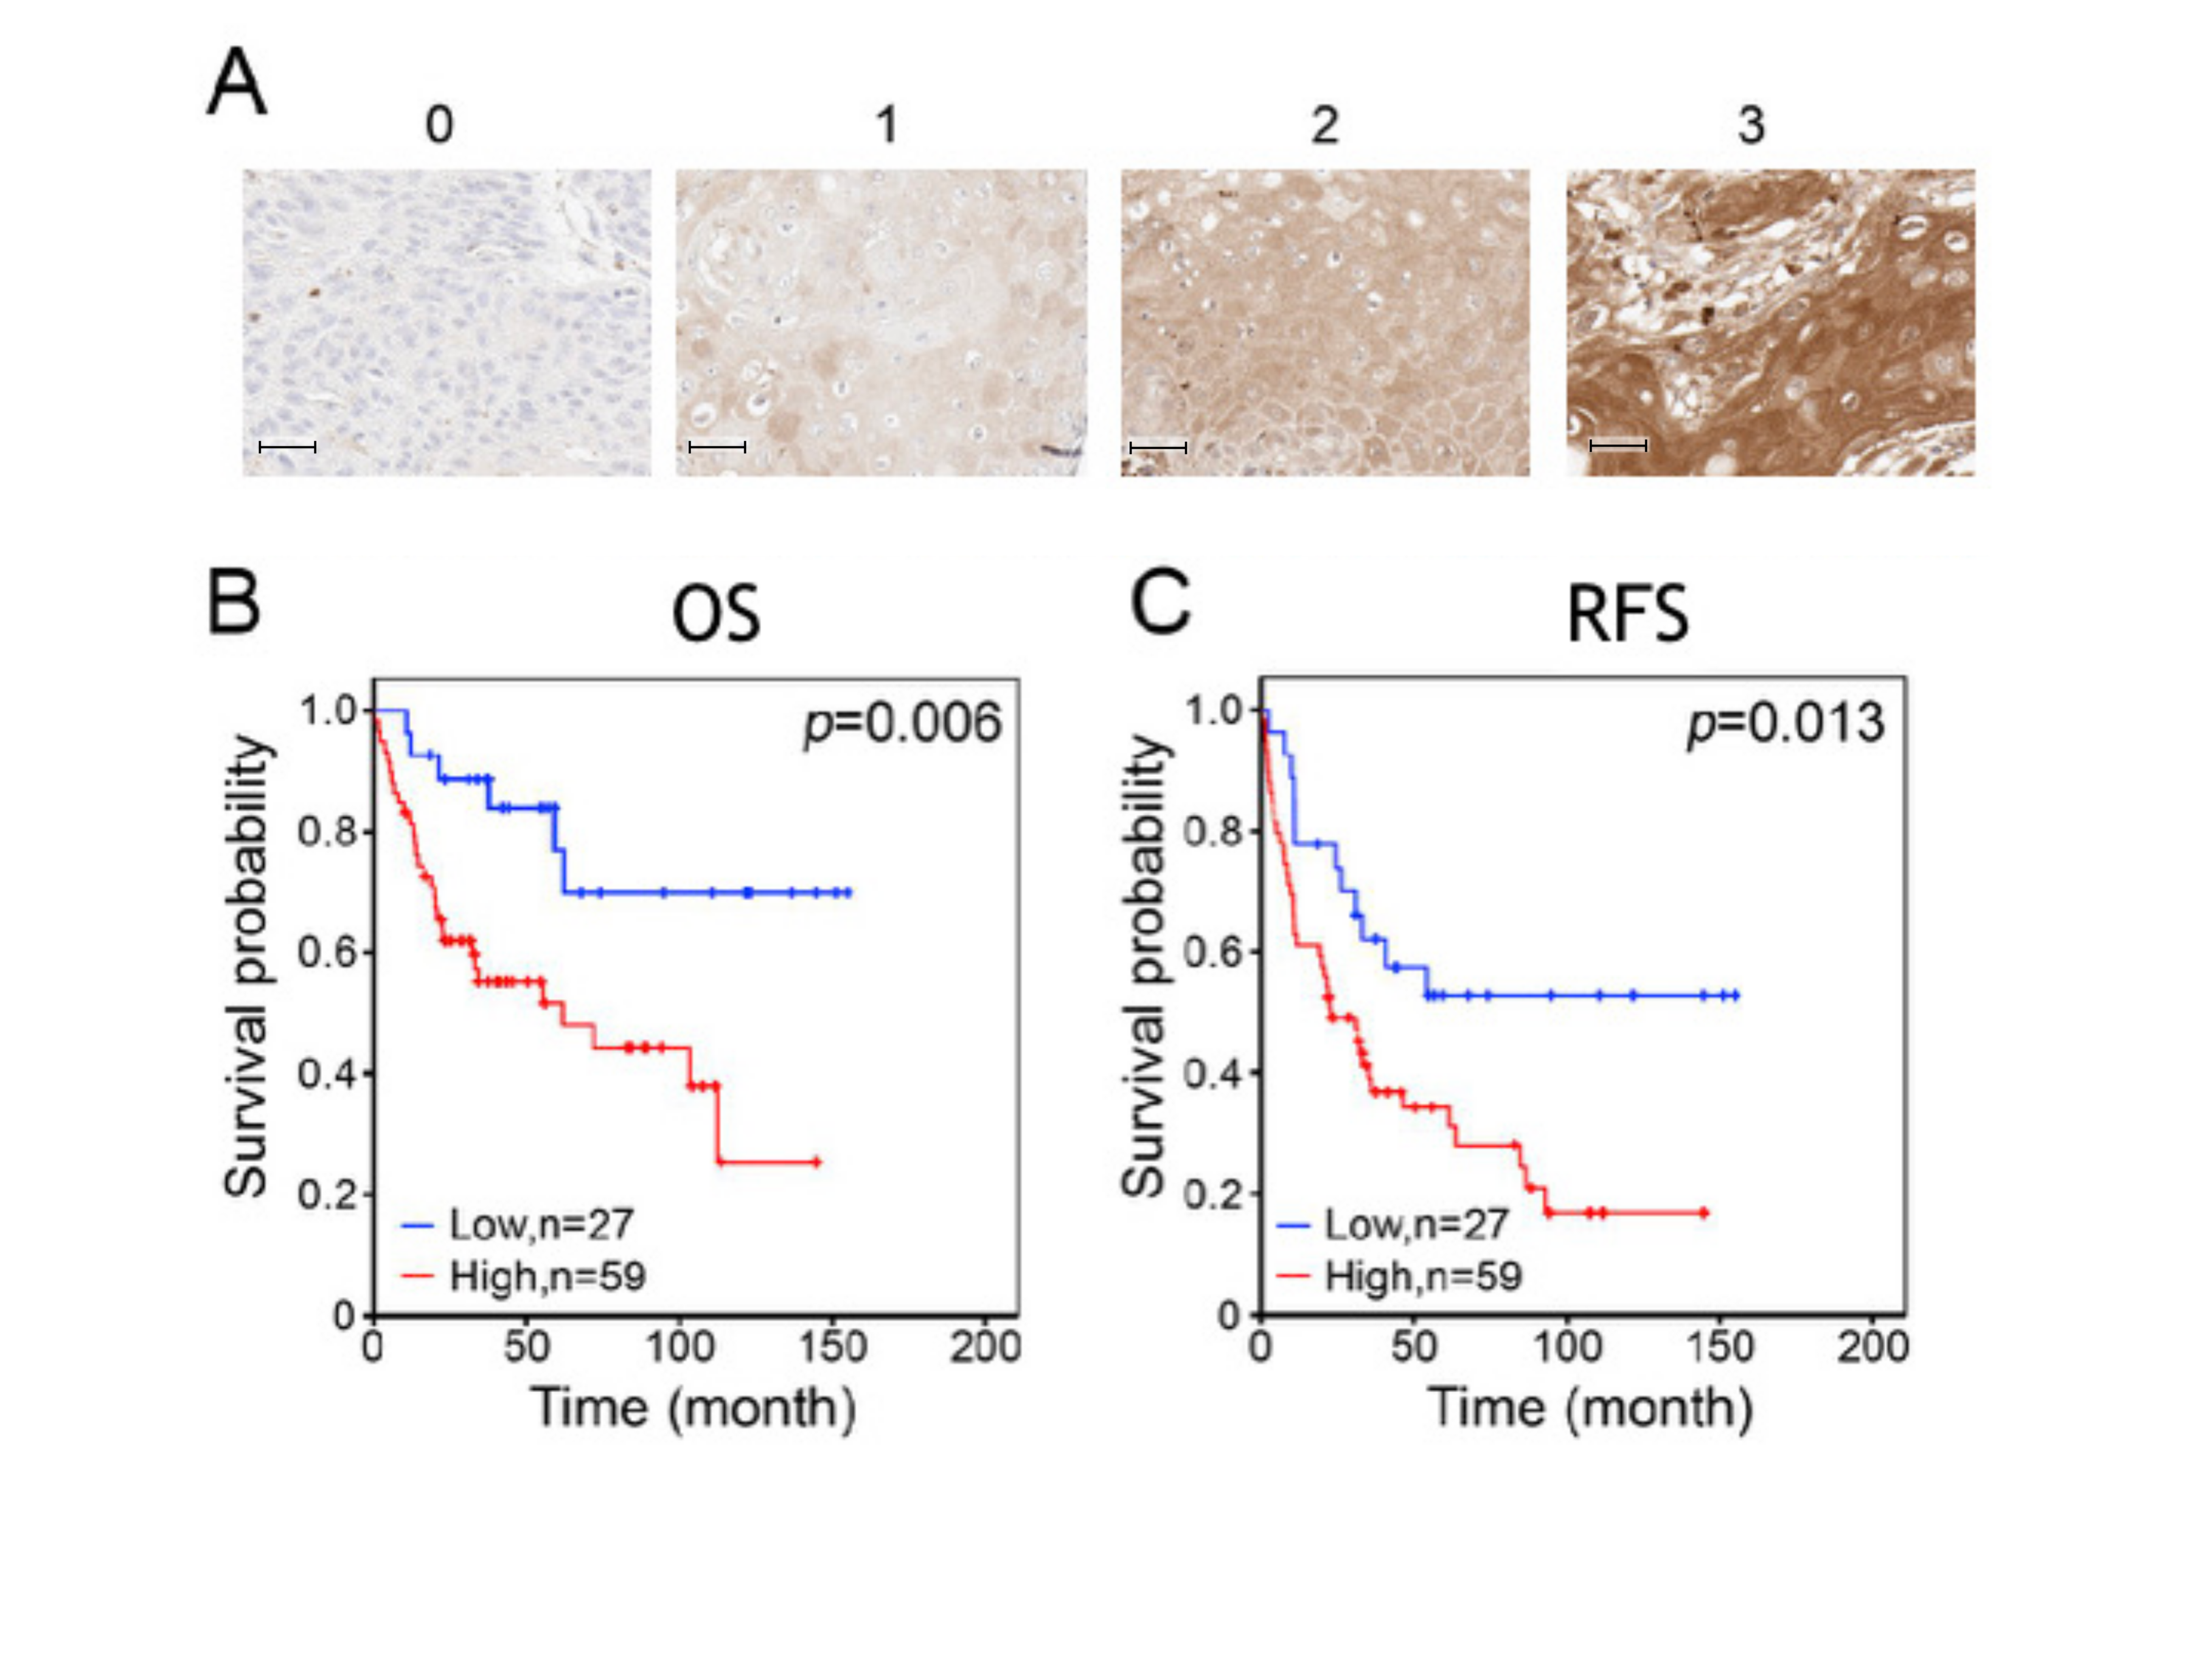
\includegraphics[height=7.0cm]{Figure-4_IHC_Hsiao.pdf}}
{\captionsetup{labelformat=empty}    
\caption{\textcolor{red}{Higher} \acrshort{tmsb4x} expression (IHC score) is correlated with \textcolor{red}{poor} prognosis in TMUH cohort (n = 86);\\[0.2cm]
while a \textcolor{red}{median cutoff} is used for Kaplan--Meier (KM) survival curve.\\[0.2cm]
\tiny
    % GSE117973 using the same platform GPL10558
(A) The representatives of \textcolor{red}{tumor tissue microarray} (scale bar = 50~\si{\um}) \\
(B) And (C) KM estimates of overall survival (OS) (\textit{p} value = 0.006) and recurrence-free survival (RFS) (\textit{p} value = 0.013) (\textit{p} value by log-rank test)}}
%    (\textcolor{red}{Red dash line}: FDR-corrected KM \textit{p} value (0.05) for 20,500 multiple comparison)
%    The 22 genes, listed on the side, had hazard ratios >$1.8$ or <$0.6$.
%    (X-axis: Kaplan--Meier survival estimates, with \acrshort{fdr}-adjusted \protect\textit{p}~values, log10 transformed; y-axis: the hazard ratio (HR) under the Cox proportional hazard regression model).

%%%\label{fig:hazards534}
\end{figure}

\clearpage


%%%%%%%%%%%%%%%%%

%%%%%%%%%%%%%%%%
\thispagestyle{headings}
\markright{Results\hfill TMSB4X IHC score in Cox's survival model \hfill}

\begin{table}[H] 
%\centering
\captionsetup{labelformat=empty}
\captionabove{%Univariate/multivariate Cox proportional hazard regression analyses on overall survival time of \hl{CAMK2N1} gene expression in HNSCC. 
% Univariate and multivariate Cox proportional hazards regression analyses on OS and RFS time of \acrshort{hnscc} (Table courtesy of~\autocite{Chi2017})
%Clinical tumor size and 
The \acrshort{tmsb4x} expression is one of significant prognostic factor in HNSCC (TMU) cohort OS/RFS, \hl{especially} in \textcolor{red}{tumor recurrence} (surgical margin or N0 $\longrightarrow$ N+) {\tiny (HR: 2.07 [1.08--3.98], \textit{p} = 0.028)}.
}

%%%\label{table:table2}
\arrayrulecolor[rgb]{0.255,0.255,0.255}


\resizebox{0.65\linewidth}{!}{%
\begin{tabular}{ll|rlll|rlll} 
\hline\hline
\multicolumn{2}{l}{Features}                & \multicolumn{4}{c}{Univariate (OS)}                                           & \multicolumn{4}{c}{Multivariate (OS)}                                                            \\ 
\hline
\multicolumn{2}{l}{}                        & HR   & \multicolumn{2}{c}{95\% CI}      & \multicolumn{1}{l}{\textit{p} value}         & HR                     & \multicolumn{2}{c}{95\% CI}      & \textit{p} value                              \\ 
\hline
T Status            & T1+T2                 & 1    &                           &      &                                     & 1                      &                           &      &                                      \\
                    & T3+T4                 & 3.22 & \multicolumn{1}{r}{1.67-} & 6.23 & \textcolor[rgb]{1,0.149,0}{0.001* } & 2.62                   & \multicolumn{1}{r}{1.31-} & 5.23 & \textcolor[rgb]{1,0.149,0}{0.006* }  \\
N Status            & N0                    & 1    &                           &      &                                     & 1                      &                           &      &                                      \\
                    & N1\textasciitilde{}N3 & 2.06 & \multicolumn{1}{r}{1.06-} & 4.01 & \textcolor[rgb]{1,0.149,0}{0.033* } & 1.73                   & \multicolumn{1}{r}{0.87-} & 3.45 & 0.121                                \\
\acrshort{tmsb4x} expression~~ & Low                   & 1    &                           &      &                                     & 1                      &                           &      &                                      \\
                    & High                  & 3.26 & \multicolumn{1}{r}{1.35-} & 7.89 & \textcolor[rgb]{1,0.149,0}{0.009* } & 3.12                   & \multicolumn{1}{r}{1.27-} & 7.63 & \textcolor[rgb]{1,0.149,0}{0.013* }  \\ 
\hline\hline
\multicolumn{2}{l}{Features}                & \multicolumn{4}{c}{Univariate (RFS)}                                          & \multicolumn{4}{c}{Multivariate (RFS)}                                                           \\ 
\hline
                    & \multicolumn{1}{l}{}  & HR   & \multicolumn{2}{c}{95\% CI}      & \multicolumn{1}{l}{\textit{p} value}         & \multicolumn{1}{l}{HR} & \multicolumn{2}{c}{95\% CI}      & \textit{p} value                              \\ 
\hline
T Status            & T1+T2                 & 1    &                           &      &                                     & 1                      &                           &      &                                      \\
                    & T3+T4                 & 1.89 & \multicolumn{1}{r}{1.08-} & 3.31 & \textcolor[rgb]{1,0.149,0}{0.027* } & 1.56                   & \multicolumn{1}{r}{0.87-} & 2.79 & 0.132                                \\
N Status            & N0                    & 1    &                           &      &                                     & 1                      &                           &      &                                      \\
                    & N1\textasciitilde{}N3 & 1.74 & \multicolumn{1}{r}{0.99-} & 3.04 & 0.050                               & 1.61                   & \multicolumn{1}{r}{0.91-} & 2.83 & 0.101                                \\
\acrshort{tmsb4x} expression   & Low                   & 1    &                           &      &                                     & 1                      &                           &      &                                      \\
                    & High                  & 2.21 & \multicolumn{1}{r}{1.16-} & 4.21 & \textcolor[rgb]{1,0.149,0}{0.016* } & \hl{2.07}                   & \multicolumn{1}{r}{1.08-} & 3.98 & \textcolor[rgb]{1,0.149,0}{0.028* }  \\ 
\hline
%\multicolumn{10}{l}{* \textit{p} value $<$ 0.05 (Cox proportional hazards regression analyses)}                                                                                                               %                             \\
%\multicolumn{10}{l}{the 95\% confidence interval (CI) for the hazard ratio (HR)}                                                                                                                          %                     \\
%\multicolumn{10}{l}{Overall survival (OS); Recurrence-free survival (RFS)}                                                                                                                                                    
\end{tabular}
} % end of \resizebox

\pbox{0.6\columnwidth}{\tiny {
(OS: overall survival; RFS: recurrence-free survival;
HR: hazard ratio;
95\% CI: 95\% confidence interval;
\protect\textit{p}~value of Cox proportional hazards regression analyses: \textcolor{red}{red \textless{} 0.05}).} %; *** \textless{} 0.001).}                              
}
%\arrayrulecolor{black}
\end{table}



%%%%
\clearpage

%%%%%%%%%%%%


\thispagestyle{headings}
\markright{Results\hfill TMSB4X experiments in vitro and in vivo \hfill}


\begin{figure}
%% cd
%\begin{adjustwidth}{-3em}{0em}
%\subfloat[Subfigure 1 list of figures text][(c)]{
    \begin{subfigure}[b]{0.4\textwidth}
%        \caption{}
        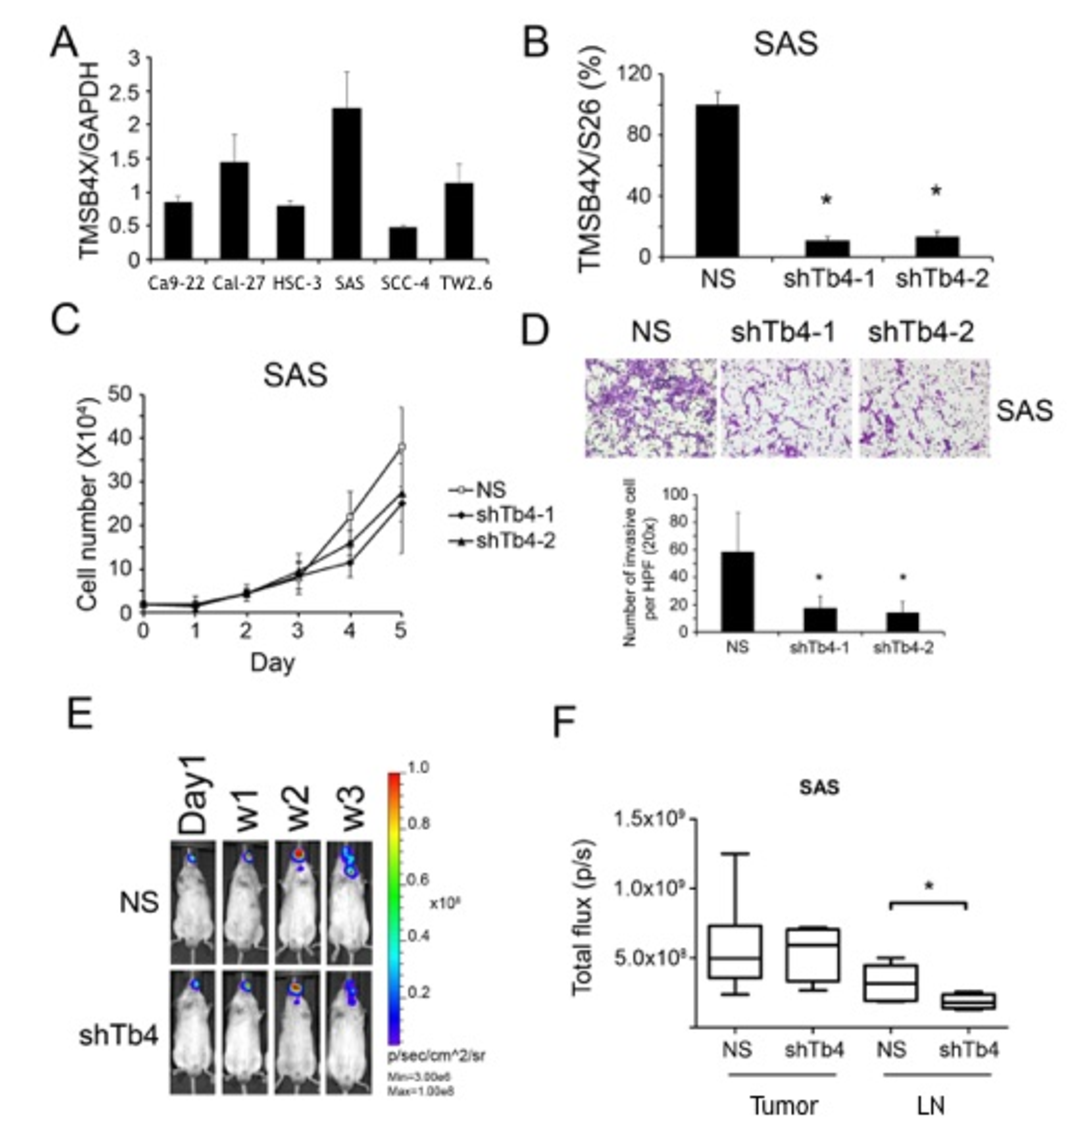
\includegraphics[width=6.5cm]{Figure-5_exp_Hsiao.pdf}
%        \caption{}
    \end{subfigure} %\hfill
    \begin{subfigure}[t]{0.10\textwidth}
        \begin{picture}(0,0) % lower left corner
            \put(10,130){\large \textcolor{red}{in vitro}} \put(10,30){\large \textcolor{red}{in vivo}}
        \end{picture}
    \end{subfigure}
%\subfloat[Subfigure 1 list of figures text][(d)]{
% \captionsetup[subfigure]{labelformat=empty}
    \begin{subfigure}[b]{0.4\textwidth}
%        \caption{}
%        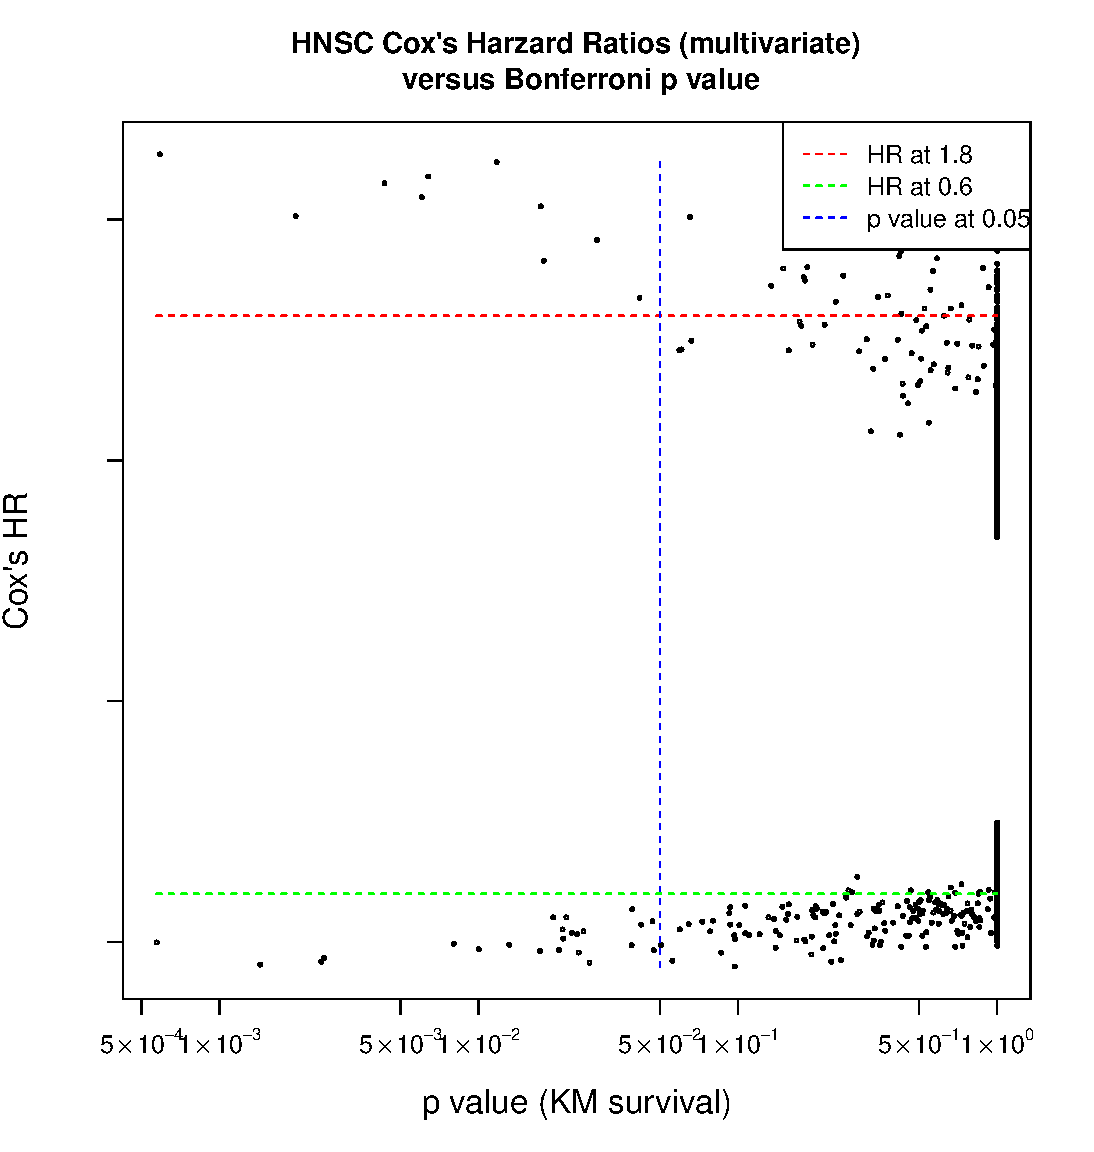
\includegraphics[width=6.5cm]{Rplot02_BonferroniP_multiHR.pdf}
        \caption*{
        (A) The aggressive SAS cells have abundant \acrshort{tmsb4x} (wild-type SAS).\\
        (B) less expression of \acrshort{tmsb4x} in knockdown clones of SAS (SAS-shTb4),\\
        (C) slower cell \hl{proliferation} in SAS-shTb4; \\
        (D) less \hl{invasion} ability in SAS-shTb4 {\tiny (by Boyden chamber assay)}.\\[0.8cm]
        (E) In bioluminescence images of the buccal orthotopic xenograft mouse model: \\
        (F) SAS-shTb4 cells has less \hl{neck metastasis} {\tiny (* \textit{p} value \textless{} 0.05 is estimated by student t-test)}.\\
        }
    \end{subfigure}
 % end of {\includegraphics}

\captionsetup{labelformat=empty}
\caption{
%After stringent restriction by Bonferroni-adjusted \textit{p}~values and Cox's HR, a few top-ranked genes were acquired by
Knockdown \acrshort{tmsb4x} in SAS cells may inhibit their cell proliferation and invasion ability in vitro, as well as suppress cervical lymph node metastasis in vivo.
}
%(TCGA: \acrlong{tcga}; HR: hazard ratio; FDR: \acrlong{fdr}).}

%\label{fig:figure2}
\end{figure}% * = no overlapping with text


\clearpage


%%%%%%%%%%%%%

\section{Summary for (A)}

\begin{outline}


\1 A biomarker---TMSB4X---is discovered by in-house patients' samples using \hl{mass spectrometry}, and validated by experiments (in vitro, in vivo);

\1 The \acrlong{tmsb4x} might promote lymph node \hl{metastasis} of HNSCC;
%\1 IPI 4980 a 5053 Dalton, Mass Spectrometry Could Omit Smaller Molecules (?)

\1 We need more biomarker by pvalueTex~\autocite{Chi2021}.
%\subsection*{The Three Biomarkers in Cancer}


%\subsubsection*{The Protein/Pathology Atlas} %still TCGA's RNA-Seq (ok)


%\subsubsection*{Literature Review} % literature (ok)


%\subsection*{Feature Selection for Survival Modeling} % Even there are many $X_1 ... X_n$ physical and social features of patients available for survival modeling in the TCGA.


%\subsection*{The Purpose of Sliding-Window Cutoff Selection}


%\subsection*{Technical Considerations}
\end{outline}



} % end of comm



%%% Chi2021 %%%%%%%%%%%%%%%
\clearpage
\section{The origin of pvalueTex (Chi2021)}

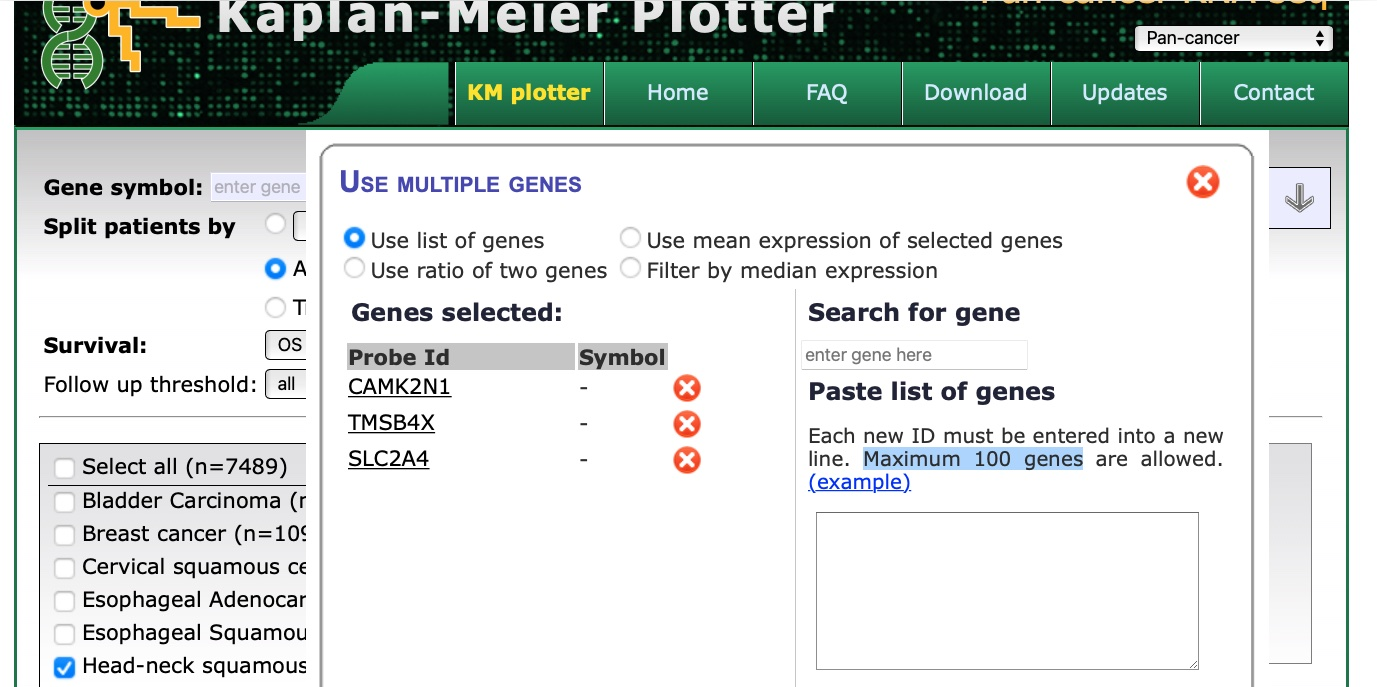
\includegraphics[width=10cm]{KM_plotter2021.jpg}\\
We are looking for biomarker candidates on KM plotter---a GUI-based web tool.\\
{\tiny \url{http://kmplot.com/analysis/index.php?p=service&cancer=pancancer_rnaseq}\\
GUI: graphic user interface, by mouse and click}

\clearpage
%
\section{Materials and Methods} %for (B) Transcriptomics} 
\subsection{Hypothesis} 
\begin{outline}

% top-down
\1 A transcriptomics research at MH laboratory (2017 to 2021);
\1 Biomarkers according to gene expression level (RNA) versus prognosis;
%    \2 spatial distribution on pathological slides, 
%    \2 time distribution on cancer stage (e.g., I II III or IV).
\1 KM plotter for TCGA: \hl{manual input} genes (100 x 200);
\1 Designing a programmatic (20,000 or 30,000 protein-coding genes) screening by \hl{sliding-window} method: Chi2021~\autocite{Chi2021}
%\1 Deep learning and holistic cancer care in the future: Chi2022
\end{outline}
%%

%%%
%\subsection{Workflow}
\thispagestyle{headings}
\markright{Workflow\hfill Our workflow---pvalueTex \hfill}
%\begin{figure}

\begin{minipage}[c]{0.45\linewidth}

%The advantages of our workflow---pvalueTex:
\begin{outline}
\1 A model for RNA-seq* analysis\\  {\tiny (*RNA-seq: \acrlong{rnaseq})} %(Figure \ref{fig:figure1})
%    \2 scanning 20,500 human protein-coding genes
\1 The Purpose of Sliding-Window Cutoff Selection
    \2 to find an \hl{optimal cutpoint} of that \acrshort{rna} expression data 
    \2 to maximize candidate mining coverage---\hl{catching more}
%    \2 identify more but sometimes weak "biomarkers"
    \2 validation by GSE65858 dataset~\autocite{Wichmann2015} ---\hl{stringent checking}
\end{outline}
\end{minipage}
% figure replaced by minipage
%\clearfloatsetup{figure}
%\floatsetup[figure]{style=no,capposition=beside,capbesideposition={center,outside},capbesideframe=yes,facing=yes}
\hfill
%\todo{python code for all figures}
\begin{minipage}[c]{0.45\linewidth}
%\label{fig:figure1}
%\floatbox[{\capbeside\thisfloatsetup{capbesideposition={right,center},capbesidewidth=.35\linewidth,capbesidesep=quad}}]{figure}[\FBwidth]
%\centering
%\widefigure, keepaspectratio
%\begin{figure}
    \centering
    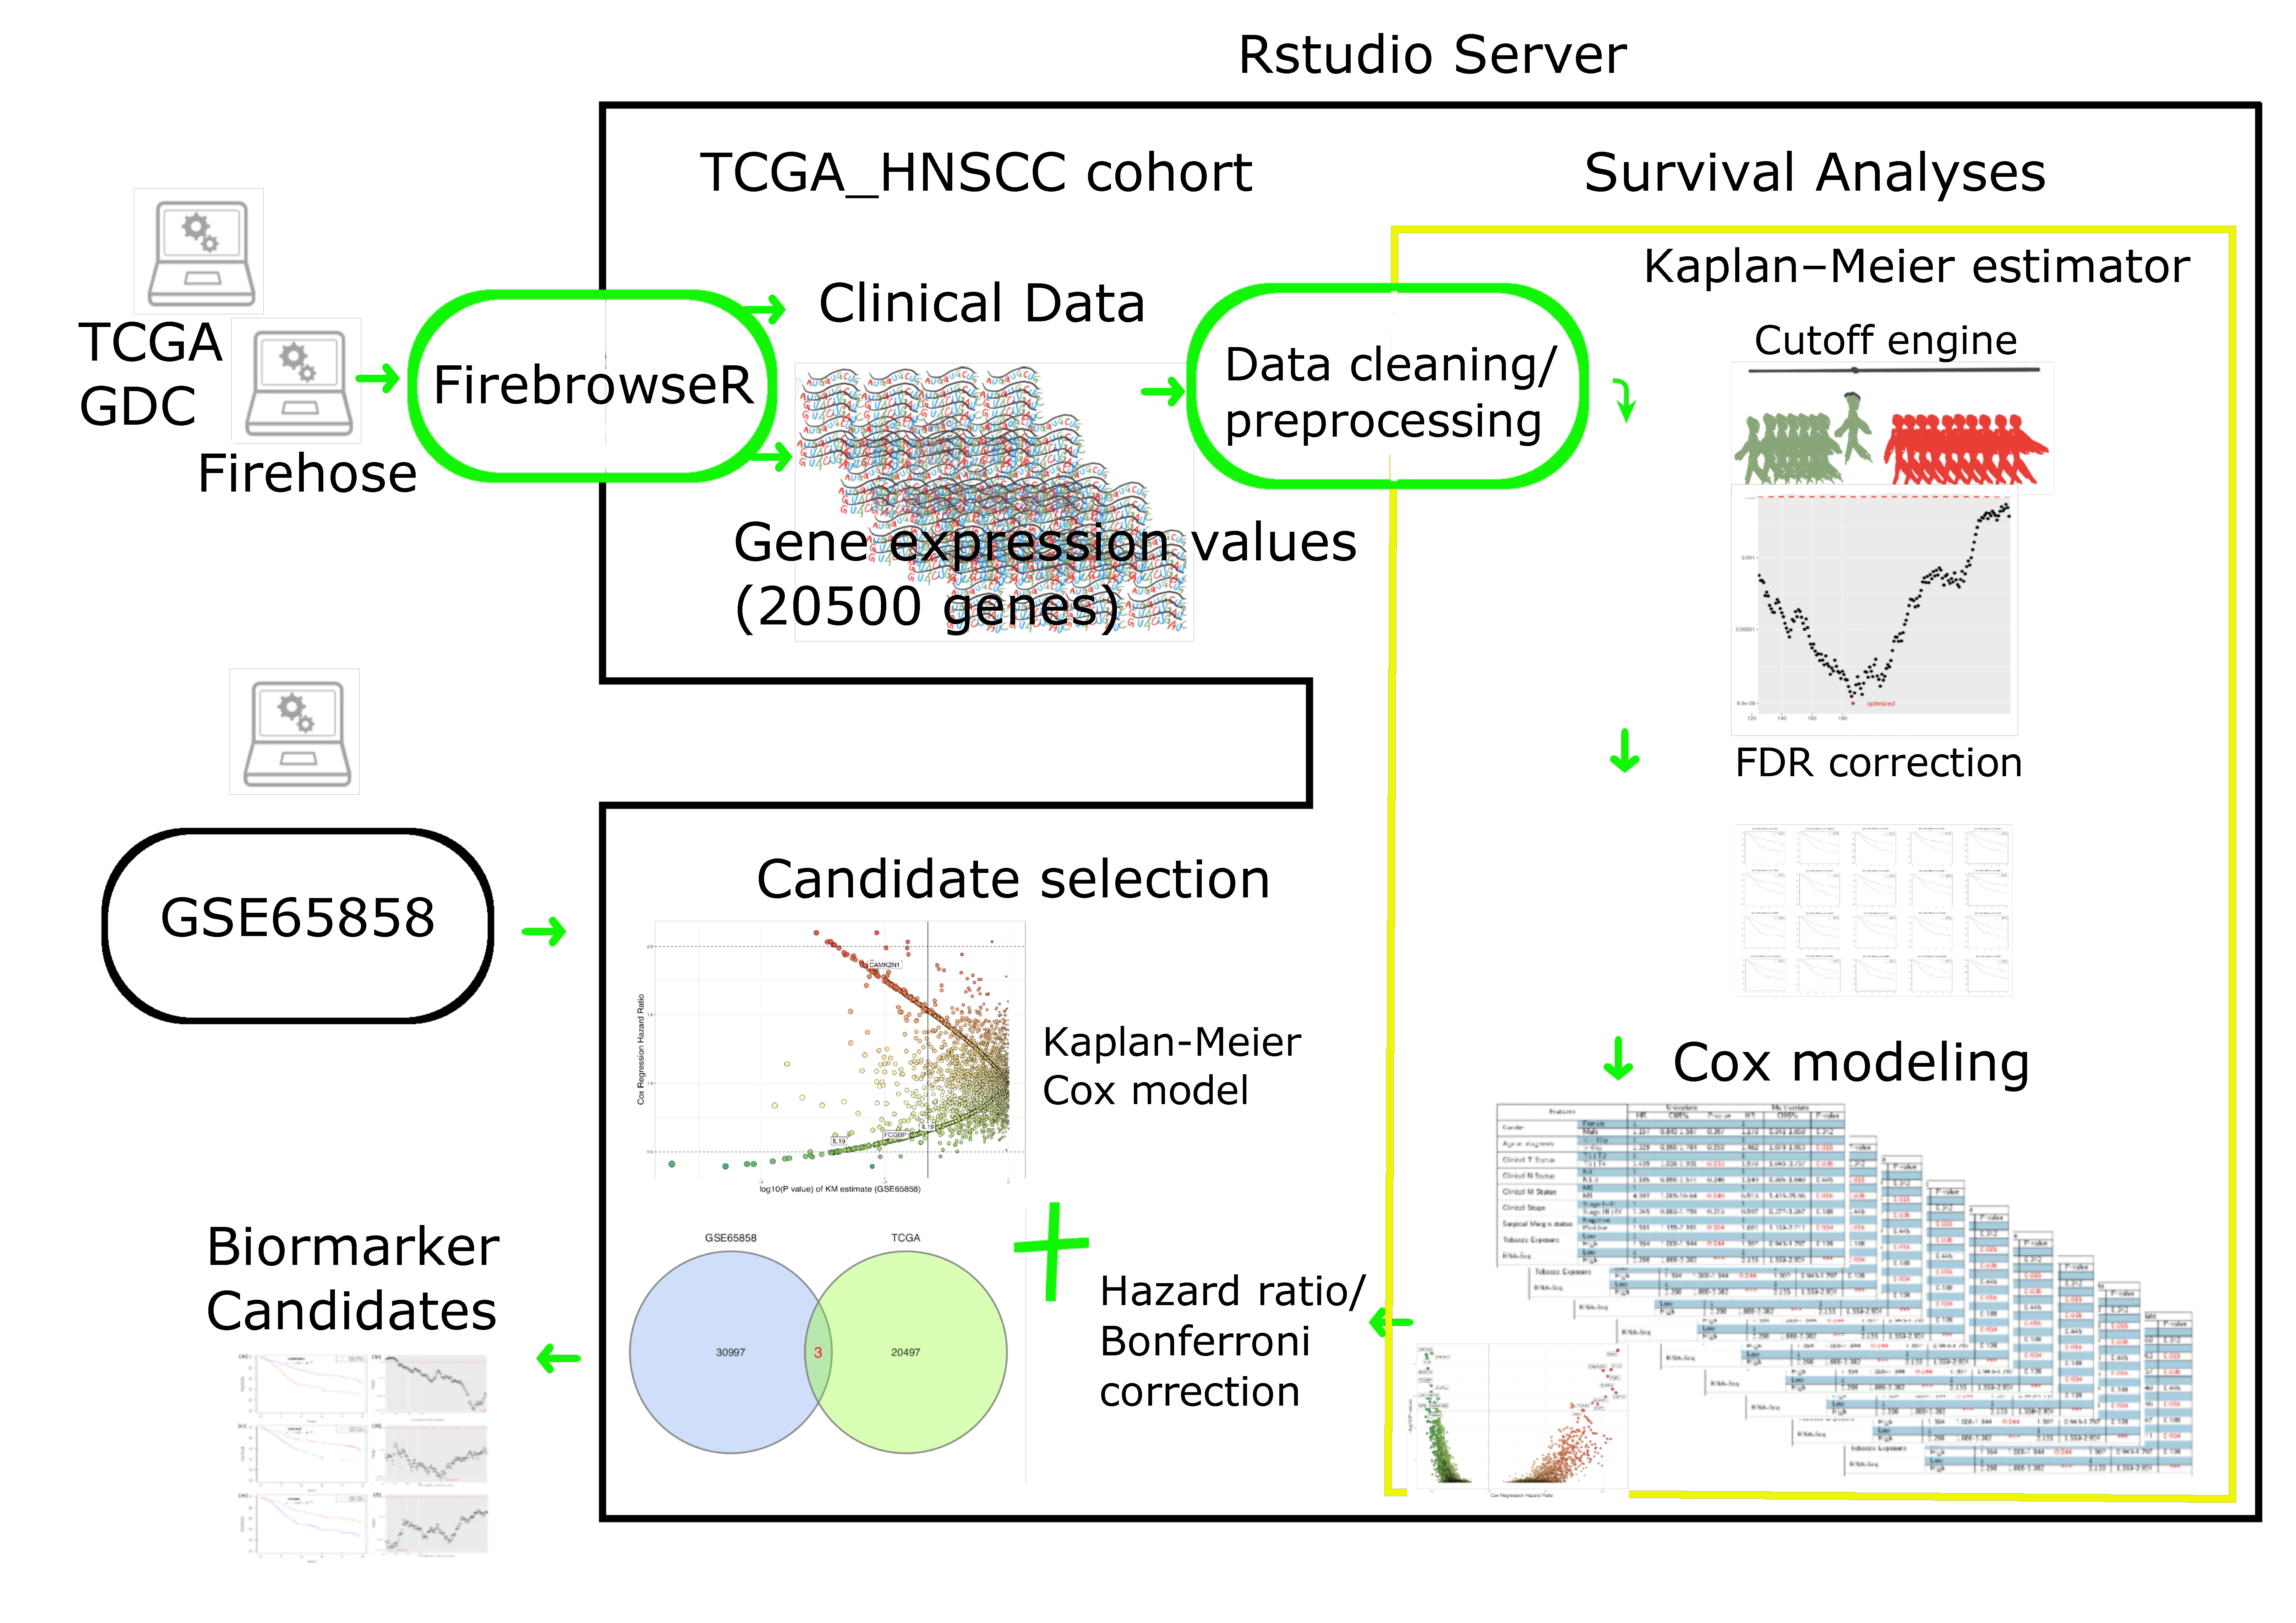
\includegraphics[width=7.5cm]{Figure_1_manuscript_workflow.pdf}
%\end{figure}
% .PDF is better than .png
%, height=8cm
%\caption % , step 1 (\textcolor{blue}{blue line}: main procedure) and step 2 (\textcolor{orange}{orange line}: analysis export).
%Step 3 (purple line: dealing with surgical margin).
%\sidecaptionvpos{c}
%{\caption{\hl{A workflow of \acrshort{hnscc} biomarker discovery.}
%The workflow includes data retrieval from the TCGA GDC data portal, data processing with merging and cleaning, and then performing the survival analyses (within \textcolor{yellow}{yellow} square).}} %The Cutoff engine (in R script: cutofFinder\_func.HNSCC.R, a serial cutoff for grouping patients with \textcolor{asparagus}{low} or \textcolor{red}{high} expression of a specific gene, to yield a collection of \protect\textit{P} values; please see Materials and Methods section for details) might calculate all possible Kaplan--Meier \protect\textit{P} values (corrected by \acrlong{fdr}, FDR, method) to find the optimal cutoff value of gene expression for subsequent Cox modeling. The candidate selection performs (1) dissecting and selection of candidate genes with further Bonferroni adjusted \protect\textit{P} values and the hazard ratios of a Cox model, based on the results from the survival analyses; (2) survival analyses of the other HNSCC dataset (GSE65858) using Kaplan--Meier estimates (with FDR corrections) and Cox modeling.\\ The biomarker candidates were consensus results of TCGA and GSE65858. (HNSCC: head and neck squamous cell carcinoma; TCGA: the Cancer Genome Atlas; RNA-Seq: RNA sequencing; GDC: Genomic Data Commons.)} } % end of caption
% Description:1) FDR correction of Kaplan--Meier \protect\textit{P} values during Cutoff finding; and 2) Bonferroni correction of Kaplan--Meier \protect\textit{P} values after Cox modeling for candidate selection.
\end{minipage}
%\end{figure}
\begin{figure}
    \centering
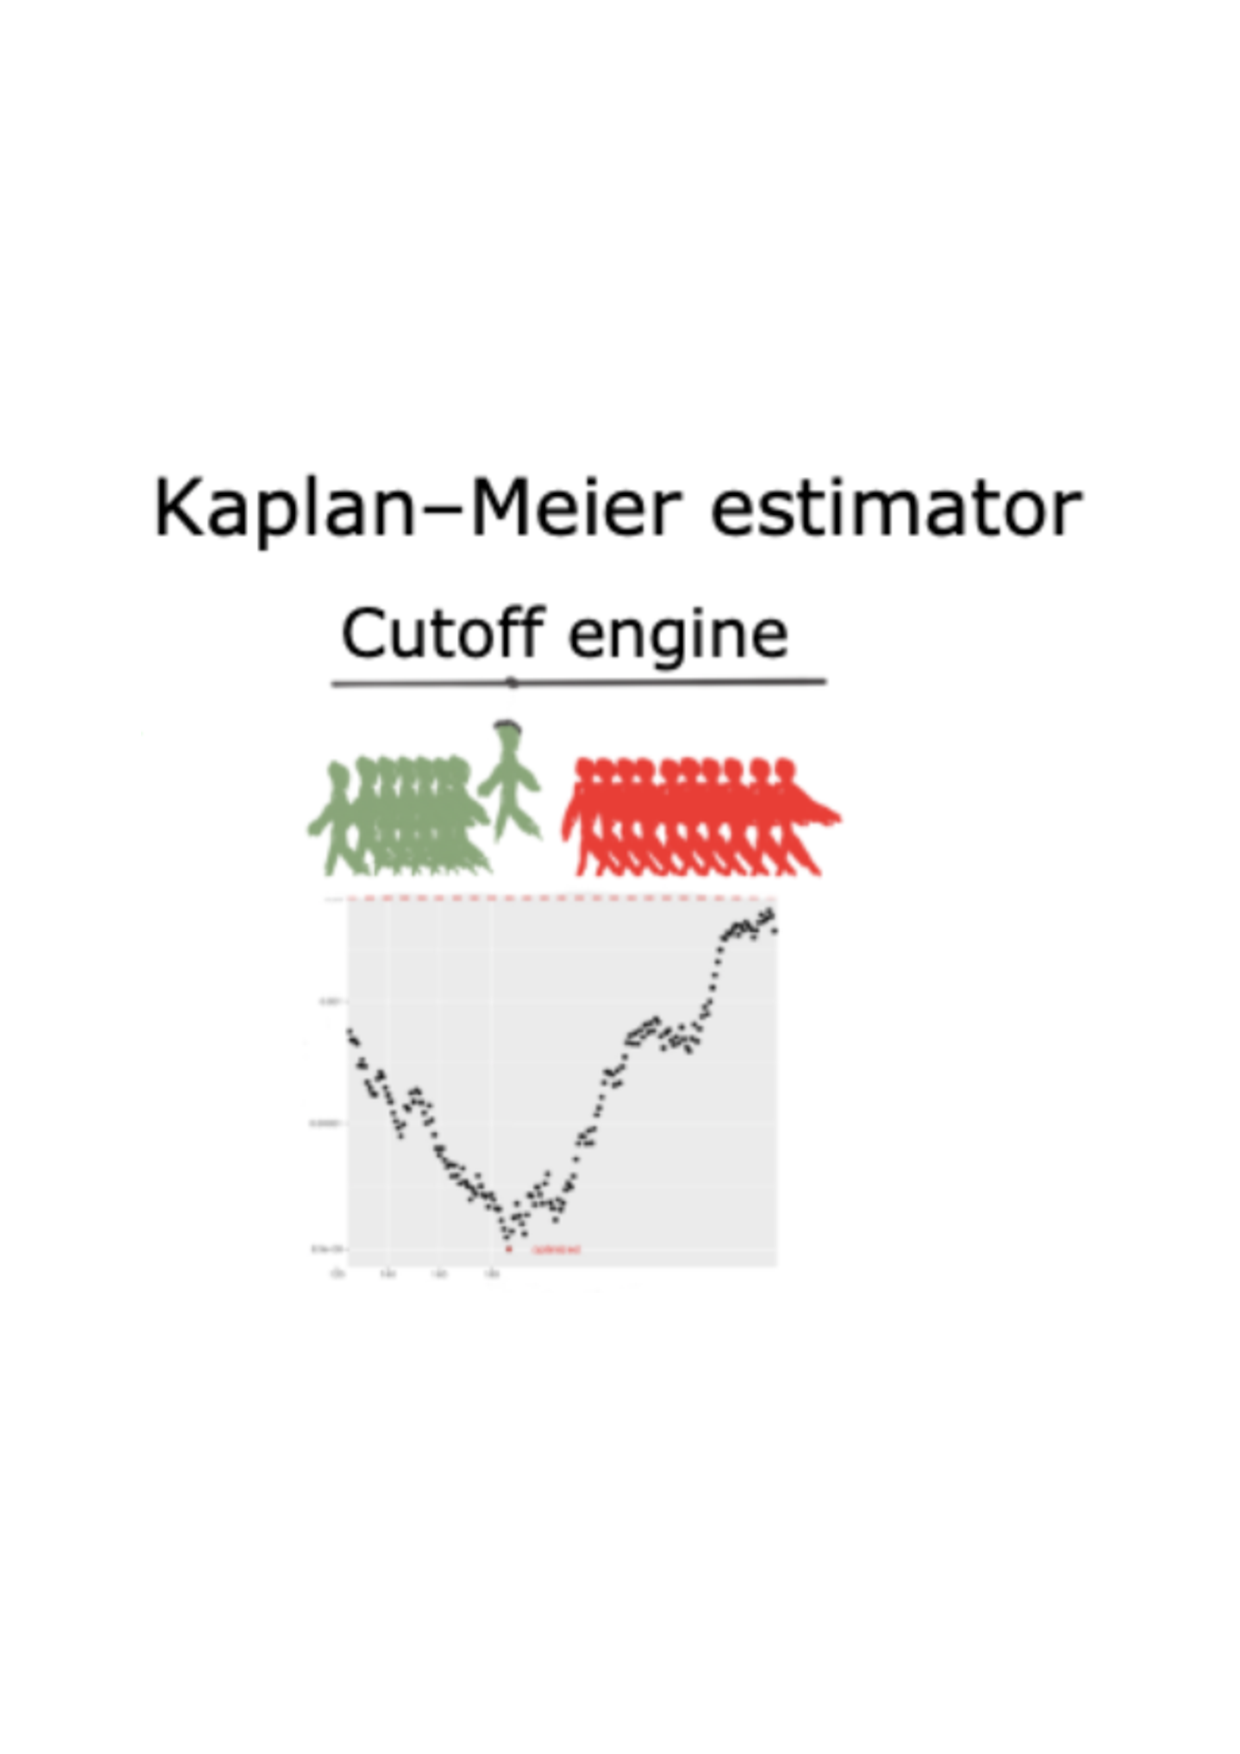
\includegraphics[height=10cm]{KM_cutoff.pdf}
%    \caption{Caption}
%    \label{fig:my_label}
\end{figure}


\clearpage
%%%%%%%%%%%%%%%%%
% automatic generation by jpm2KOMO-script.py
%% [2011/08/08]
%%%%%%%

%\section{Materials and Methods}

\subsection{Cutoff Finder Core Engine}
\thispagestyle{headings}
\markright{Statistics \hfill HNSCC in \acrfull{tcga} database \hfill}%\hfill Why TCGA dataset? \hfill}


%\subsection{Statistical Consideration for Survival Analysis}
\begin{minipage}[c]{0.45\linewidth}

%\large
\begin{outline}

\1 sliding-window cutoff selection
    \2 a \hl{serial cut} at 30\%-70\% for KM estimates
%    \2 log-rank test 
    \2 the lowest one in \textit{p}-value plot for each gene
\2  \acrfull{fdr} ($ < 0.05$) correction {\tiny ~\autocite{Benjamini1995a}} to control the type I error of multiple test 
%\1 Bonferroni correction for candidate selection


\end{outline}
\end{minipage}
\begin{minipage}[c]{0.35\linewidth}
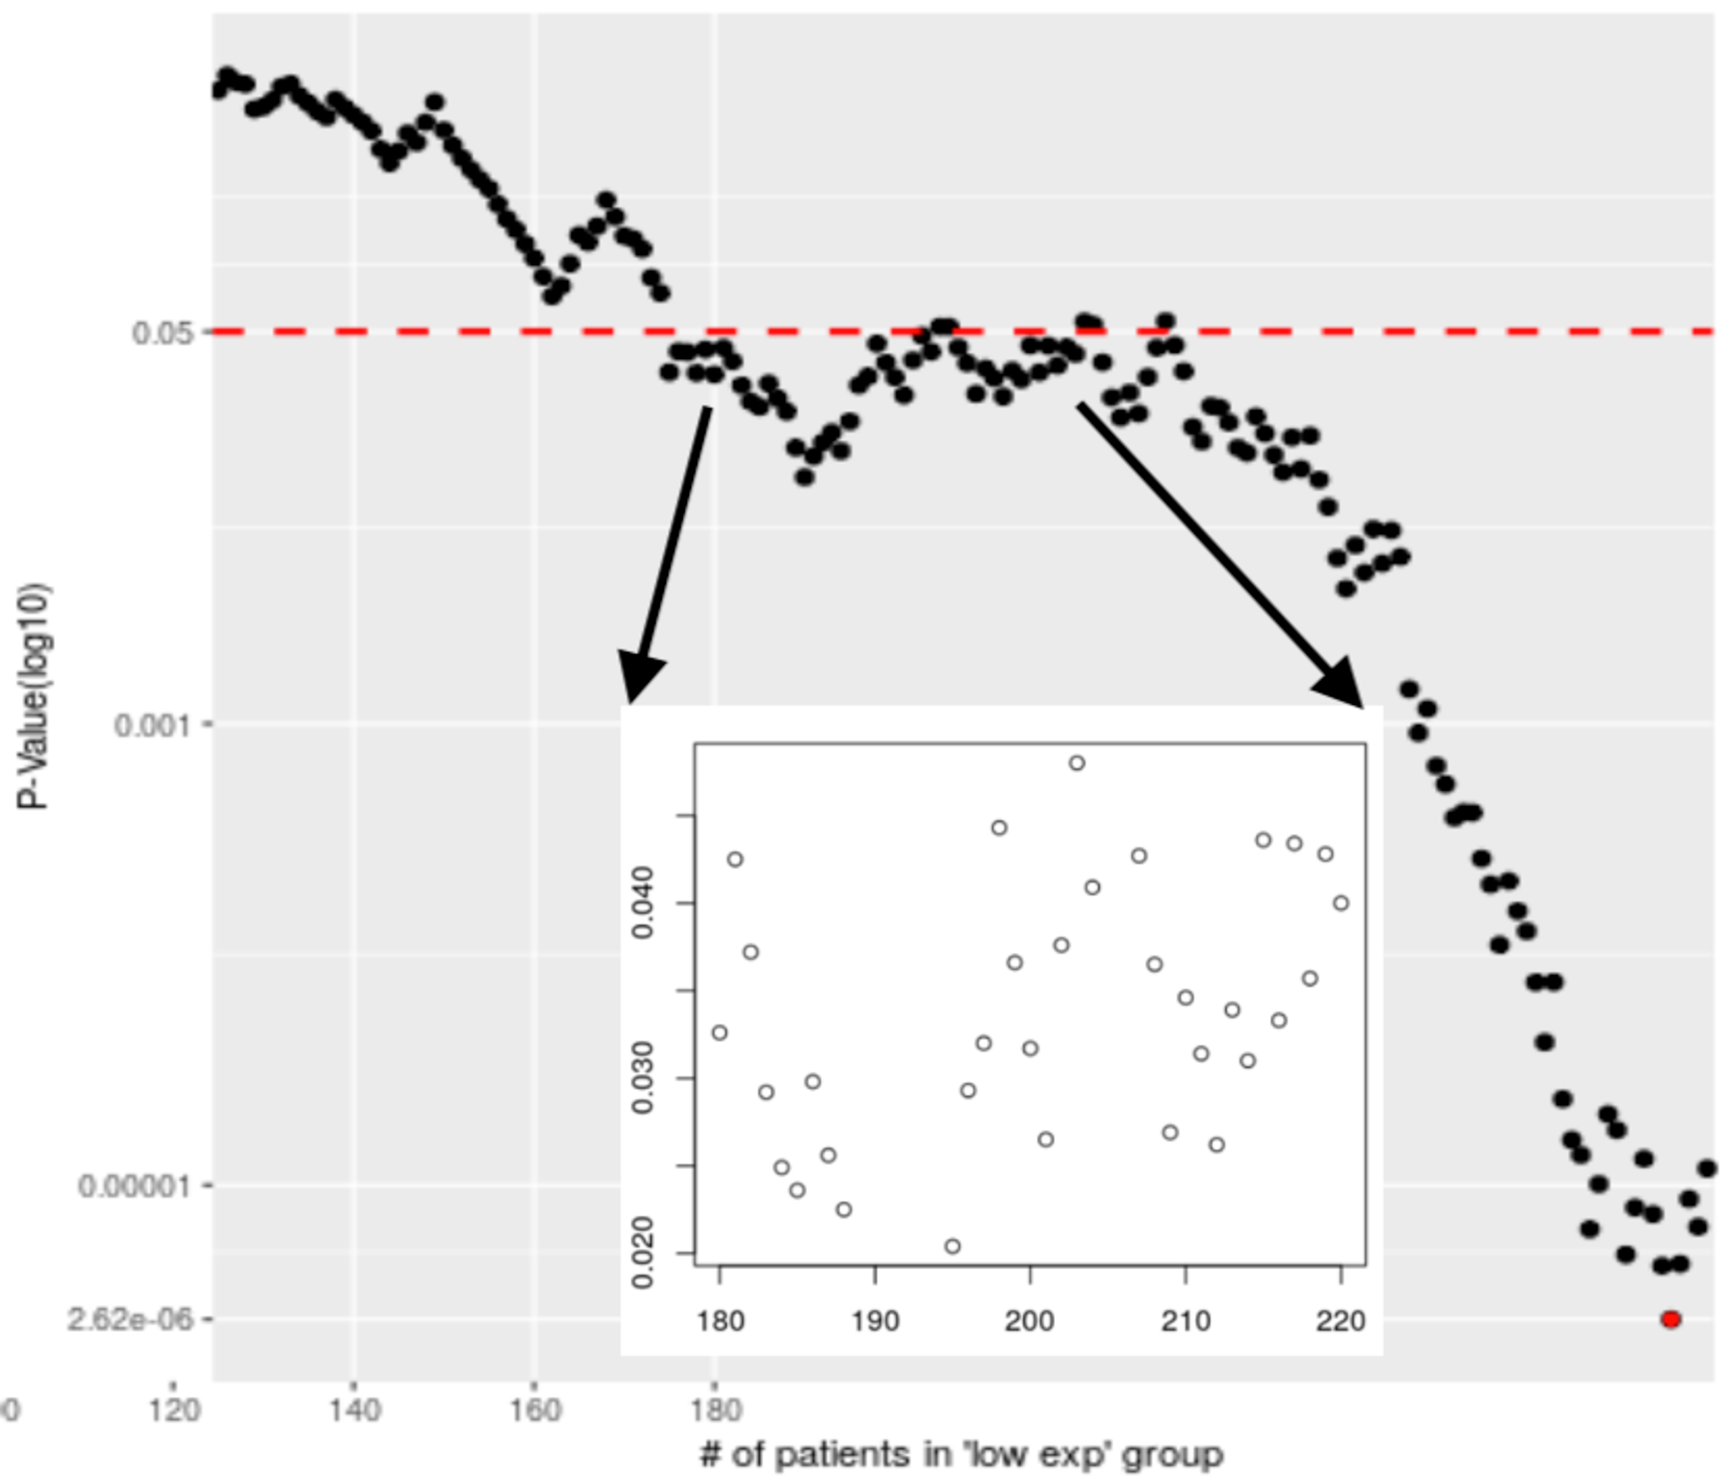
\includegraphics[width=7.5cm]{Rplot_pvaluePlot_NDFIP1.pdf}
\end{minipage}



\clearpage

\subsection{Validation Cohort}

Initial manuscript at preprint services: \url{https://www.researchsquare.com/article/rs-122012/new/v1}, and \url{https://www.preprints.org/manuscript/202107.0171/v1}

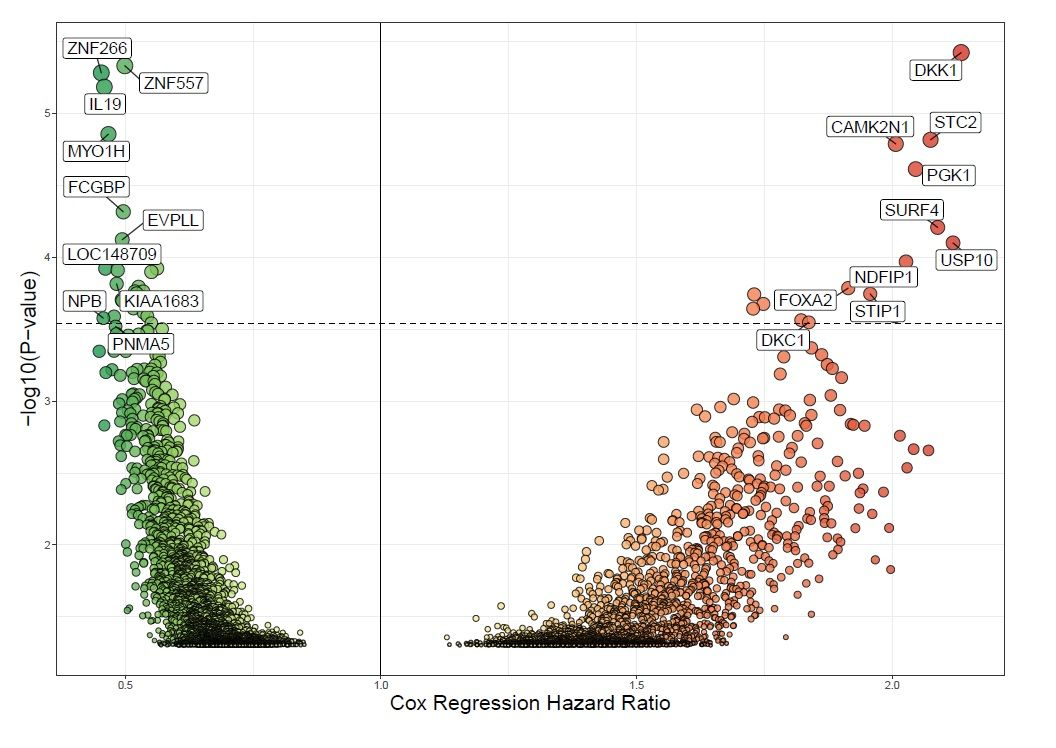
\includegraphics[width=8cm]{fcaf149553b93b72bd044c41.jpg} {\tiny $[0.5<$Hazard ratio$<1.5]$}

Reviewer's comment: "the validation rate is relatively low, and the usability of the biomarkers is questionable."\\

We found GSE65858 dataset.

\clearpage
%%%
\section{Results} % for (B)}


\clearpage

\thispagestyle{headings}
\markright{Results\hfill 39 preliminary biomarkers  \hfill}

\begin{figure}[ht]

\floatbox[{\capbeside\thisfloatsetup{capbesideposition={right,center},capbesidewidth=.35\linewidth,capbesidesep=quad}}]{figure}[\FBwidth]
    %\centering
{    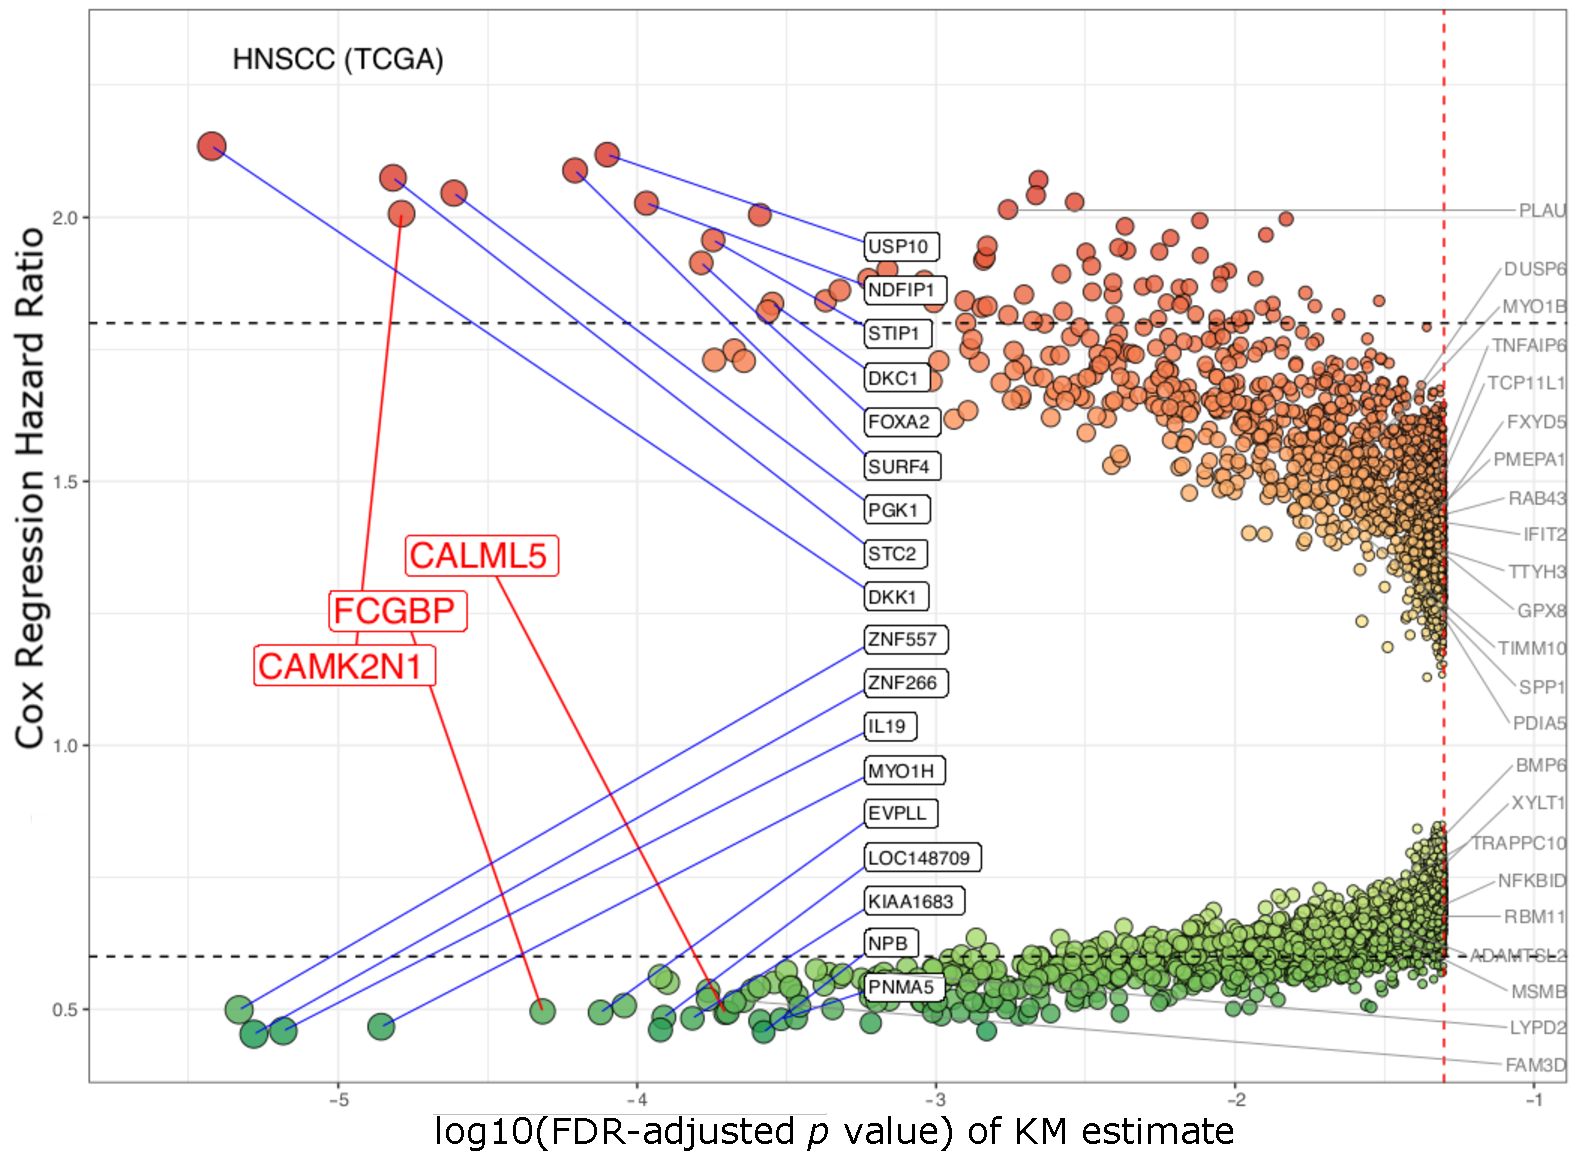
\includegraphics[width=9cm]{Rplot_TCGA_HNSCC_CoxHR_CAMK2N1_top3FDRKM.pdf}}
{\captionsetup{labelformat=empty}    
\caption{A volcano plot of preliminary candidate genes in HNSCC \hl{discovery cohort (TCGA)} {\tiny (Bonferroni-adjusted KM \textit{p} values \hl{$< 0.05$})}.\\
{\tiny    \textcolor{red}{Red spots}: HR > 1.0;\\
    \textcolor{green}{Green spots}: HR < 1.0;\\
    \textcolor{red}{Red dash line}: FDR \textit{p} = 0.05.}\\
%X axis: unadjusted \protect\textit{p}~value of Kaplan--Meier survival (-log10 transformed).
%Y axis: multivariate hazard ratio from Cox proportional regression model.
%Dotted line: significant Bonferroni corrected \protect\textit{p}~value. 
%\textcolor{red}{Red dots} mark 10 genes (unvalidated), which impact on poor prognosis ($HR>=1.5$). \textcolor{green}{Green dots} mark 10 genes (unvalidated), which affect on better survival ($HR<=0.5$).
%    This cohort was applied for exploration of the candidate biomarkers.
%    A total of 9416 genes had %\acrshort{fdr}-
%    unadjusted \protect\textit{p}~values of less than 0.05.
    \textcolor{red}{CAMK2N1}, \textcolor{green}{CALML5}, \textcolor{green}{FCGBP}, and  other genes (marked in \textcolor{black}{black square}) had hazard ratios (HRs) \hl{>$1.8$ or <$0.6$}.
%    The 22 genes, listed on the side, had hazard ratios between 0.6 and 1.5.
%    (X-axis: Kaplan--Meier survival estimates, with \acrshort{fdr}-adjusted \protect\textit{p}~values (log10 transformed);
%y-axis: HR of Cox proportional hazard regression model.)
    }}
%%%\label{fig:hazards3}
\end{figure}


%
\clearpage

\thispagestyle{headings}
\markright{Results\hfill Three candidate biomarkers  \hfill}

\begin{figure}[ht]
\floatbox[{\capbeside\thisfloatsetup{capbesideposition={right,center},capbesidewidth=.35\linewidth,capbesidesep=quad}}]{figure}[\FBwidth]
   % \centering
{    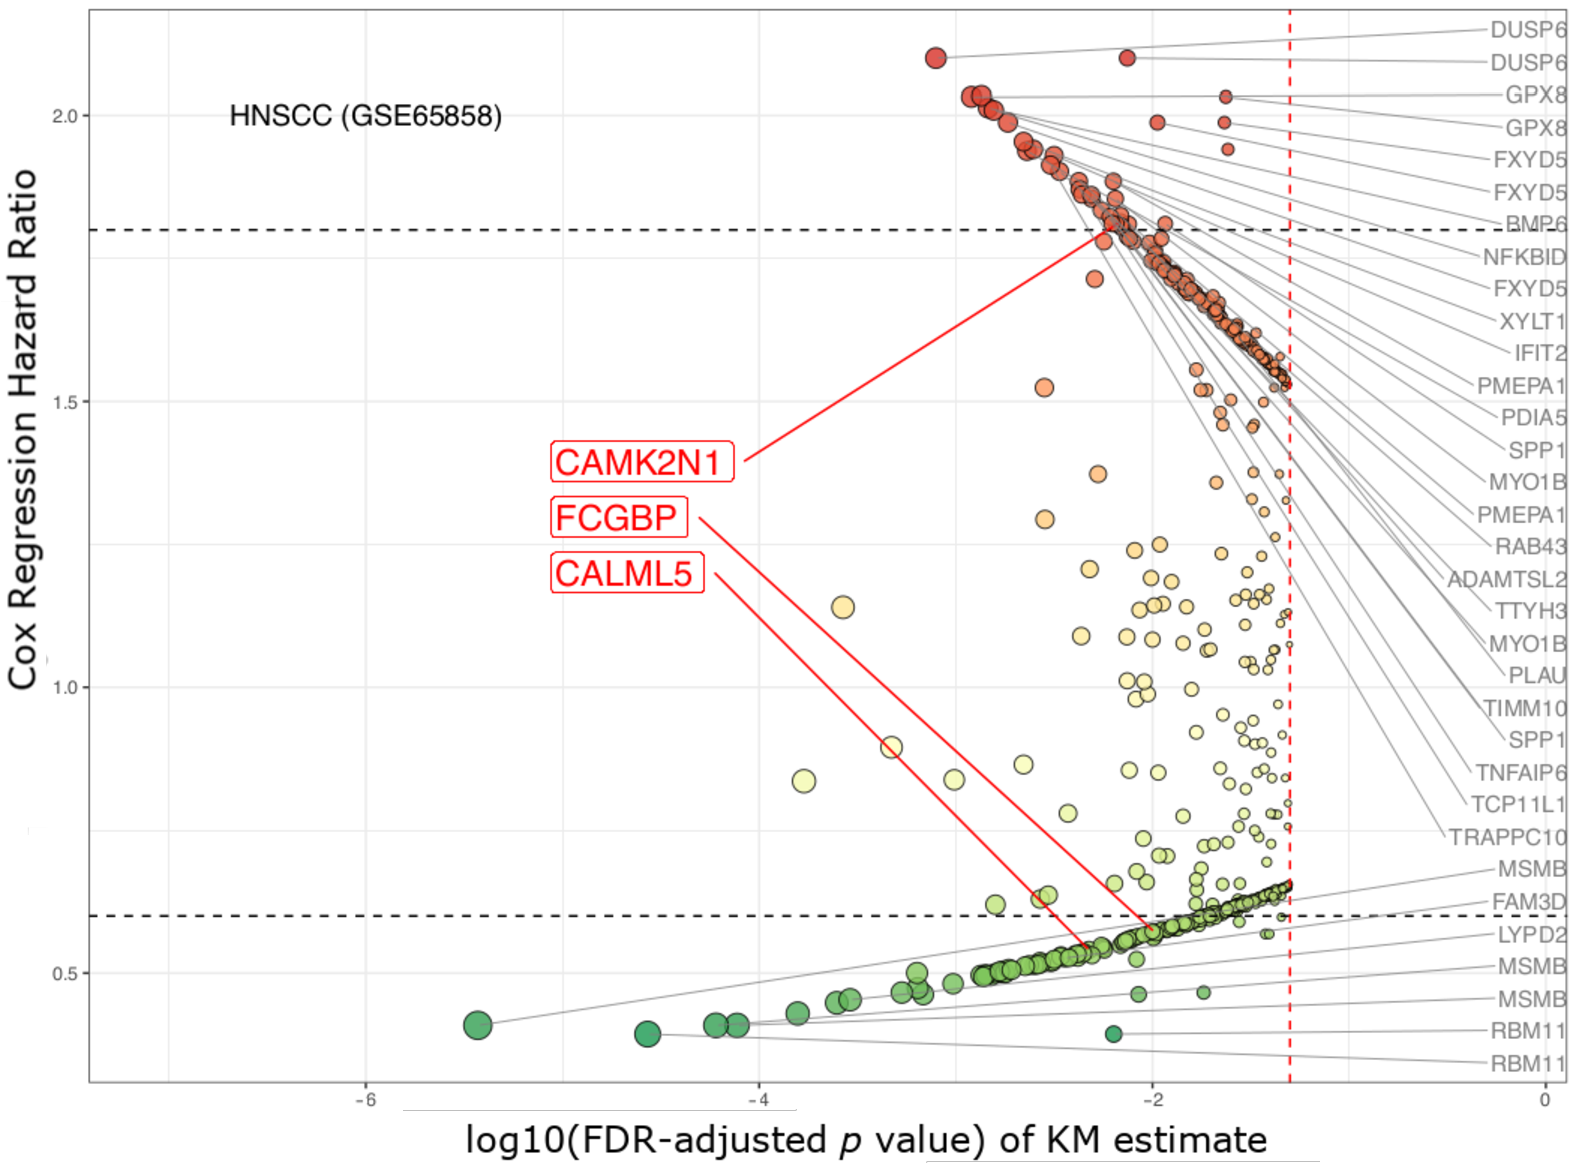
\includegraphics[width=9cm]{Rplot_GSE65858_CoxHR_CAMK2N1_top3FDRKM.pdf}}
{\captionsetup{labelformat=empty}    \caption{Volcano plot of genes in survival analyses of a HNSCC \hl{validation cohort (GSE65858)}.\\
    % GSE117973 using the same platform GPL10558
The candidate genes---\textcolor{red}{CAMK2N1}, \textcolor{green}{CALML5}, and \textcolor{green}{FCGBP}---was confirmed by hazard ratios (HRs) \hl{>$1.8$ or <$0.6$}.\\
%    In total, 534 genes had \acrshort{fdr}-adjusted \protect\textit{p}~values less than 0.05
{\tiny    (\textcolor{red}{Red dash line}: FDR-corrected KM \textit{p} value (0.05) for 20,500 multiple comparison)}
%    The 22 genes, listed on the side, had hazard ratios >$1.8$ or <$0.6$.
%    (X-axis: Kaplan--Meier survival estimates, with \acrshort{fdr}-adjusted \protect\textit{p}~values, log10 transformed; y-axis: the hazard ratio (HR) under the Cox proportional hazard regression model).
    }}
%%%\label{fig:hazards534}
\end{figure}
%%%%%%%%%%%%%%%%%%%%%%%

\clearpage


% top 3 genes
\thispagestyle{headings}
\markright{Results \hfill KM and Cox in TCGA \hfill}

\begin{table}[H] 
%\centering
%\caption{The top 3 genes with prognostic impacts on HNSCC.}% (ranked by Bonferroni-adjusted \protect\textit{p}~values}

%%%\label{tab:newTable1}
\resizebox{0.9\linewidth}{!}{% \textwidth
\begin{tabular}{|l|l|l|c|c|c|c|c|c|}
\noalign{\hrule height 1.0pt}
\multicolumn{1}{|c|}{} &
  \multicolumn{2}{c|}{} &
  \multicolumn{2}{c|}{\textbf{Kaplan--Meier Survival}} &
  \multicolumn{2}{c|}{\textbf{Cox Univariate}} &
  \multicolumn{2}{c|}{\textbf{Cox Multivariate}} \\ \cline{4-9} 
\multicolumn{1}{|l|}{\multirow{-2}{*}{\textbf{Gene ID}}} &
  \multicolumn{2}{l|}{\multirow{-2}{*}{\textbf{Gene Descriptio}n}} &
  \begin{tabular}[c]{@{}c@{}}\textbf{FDR}\\ \textbf{\protect\textit{p}~Value}\end{tabular} &
  \begin{tabular}[c]{@{}c@{}}\textbf{Bonferroni}\\ \textbf{\protect\textit{p}~Value}\end{tabular} &
  \textbf{HR *} &
  \textbf{CI95\%} &
  \textbf{HR *} &
  \textbf{CI95\%} \\ 
  \hline
CAMK2N1 &
  \multicolumn{2}{l|}{\begin{tabular}[c]{@{}l@{}}calcium/calmodulin-\\ dependent protein\\ kinase II inhibitor 1\end{tabular}} &
  \num{1.63e-5} & %2.9e-7} &
  0.002 &
  \textcolor{red}{2.101} &
  1.572--2.809 &
  \textcolor{red}{2.007} &
  1.490--2.704 \\ \hline
CALML5 &
  \multicolumn{2}{l|} {\acrlong{CALML5}} &
   \num{1.97e-4} & %\num{6.54e-6} & %3.7e-7} &
   0.039 &
   \textcolor{green}{0.51} &
   0.379--0.686 &
   \textcolor{green}{0.493} &
   0.364--0.667 \\ \hline
FCGBP &
  \multicolumn{2}{l|}{\begin{tabular}[c]{@{}l@{}}Fc fragment of\\  IgG binding protein\end{tabular}} &
   \num{4.83e-5} & %1.2e-6} &
   0.008 &
   \textcolor{green}{0.484} &
   0.359--0.653 &
   \textcolor{green}{0.496} &
   0.366--0.674 \\ 
\noalign{\hrule height 1.0pt}
%\multicolumn{9}{|l|}{} \\
%\multicolumn{9}{|l|}%{\multirow{-0}{*}
%{\begin{tabular}[c]{@{}l@{}}
%
%\end{tabular}
%%}\\ % within \multirow
%} \\ % within \multicolumn
%\hline
%\multicolumn{9}{|l|}{ \\ \hline

\end{tabular}%
}
\pbox{0.8\columnwidth}{\footnotesize
~\\
The top 3 genes with prognostic impacts on HNSCC.\\
\hl{Selection criteria} (fit all):\\
(1) Kaplan--Meier Bonferroni-adjusted~\hl{\textit{p} \textless~0.05} in both \underline{discovery TCGA} and \underline{validation GSE65858} cohorts; \\
(2) Cox's univariate and multivariate \hl{HR \textgreater{}= 1.8 or \textless{}= 0.6} in both \underline{discovery TCGA} and \underline{validation GSE65858} cohorts.\\ 
%(3) Cox's univariate and multivariate HR \textgreater{}= 1.8 or \textless{}= 0.6 in GSE65858 cohort.\\
{\tiny (*~Cox's model: \textit{p} \textless 0.001; HR: hazard ratio; CI95\%: 95\% confidence interval; FDR: \acrlong{fdr}.)}
}

\end{table}
%\clearpage
\clearpage


%%%%%%%%%%%%%%%%%%%%%%%%%%%%%%
%% table 1
\clearpage
%
\thispagestyle{headings}
\markright{Results\hfill Overall survival of CAMK2N1  \hfill}

\begin{table}[H] 
%\centering
\captionsetup{labelformat=empty}
\captionabove{%Univariate/multivariate Cox proportional hazard regression analyses on overall survival time of \hl{CAMK2N1} gene expression in HNSCC. 
Clinical (T)umor size, positive surgical margin, and CAMK2N1 expression are independent prognostic factors in HNSCC (TCGA) cohort.}

%%%\label{table:table2}
\arrayrulecolor[rgb]{0.255,0.255,0.255}


\resizebox{0.55\linewidth}{!}{%
\begin{tabular}{|l|l|c|c|c|c|c|c|} 
\noalign{\hrule height 1.0pt}
%\begin{tabularx}{\textwidth}{|p{2.5cm}|l|l|l|l|l|l|l|} 
%\arrayrulecolor{black}\cline{1-2}
\arrayrulecolor[rgb]{0.255,0.255,0.255}
\cline{3-8}
\multicolumn{2}{|l!{\color{black}\vrule}}{\multirow{2}{*}{\textbf{Features}}}                                                          & \multicolumn{3}{c|}{\textbf{Univariate}}                                                                                                                                                                                                                & \multicolumn{3}{c|}{\textbf{Multivariate}}                                                                                                                                                                                                               \\ 
\cline{3-8}
\multicolumn{2}{|l!{\color{black}\vrule}}{}                                                                                   & \multicolumn{1}{l!{\color{black}\vrule}}{\textbf{HR}}                                   & \multicolumn{1}{c!{\color{black}\vrule}}{\textbf{CI95\%}}                              & \multicolumn{1}{l!{\color{black}\vrule}}{\textbf{\protect\textit{p}~Value}}                    & \multicolumn{1}{l!{\color{black}\vrule}}{\textbf{HR}}                                   & \multicolumn{1}{c!{\color{black}\vrule}}{\textbf{CI95\%}}                              & \multicolumn{1}{l!{\color{black}\vrule}}{\textbf{\protect\textit{p}~Value}}                     \\ 
\arrayrulecolor{black}\hline
\multirow{2}{*}{Gender}                 & \multicolumn{1}{l!{\color{black}\vrule}}{{\cellcolor[rgb]{0.62,0.812,0.878}}Female} & \multicolumn{1}{l!{\color{black}\vrule}}{{\cellcolor[rgb]{0.62,0.812,0.878}}1} & \multicolumn{1}{l!{\color{black}\vrule}}{{\cellcolor[rgb]{0.62,0.812,0.878}}} & \multicolumn{1}{l!{\color{black}\vrule}}{{\cellcolor[rgb]{0.62,0.812,0.878}}} & \multicolumn{1}{l!{\color{black}\vrule}}{{\cellcolor[rgb]{0.62,0.812,0.878}}1} & \multicolumn{1}{l!{\color{black}\vrule}}{{\cellcolor[rgb]{0.62,0.812,0.878}}} & \multicolumn{1}{l!{\color{black}\vrule}}{{\cellcolor[rgb]{0.62,0.812,0.878}}}  \\ 
\cline{2-8}
                                        & Male                                                                                & 1.157                                                                          & 0.843--1.587                                                                   & 0.367                                                                         & 1.076                                                                          & 0.767--1.510                                                                   & 0.671                                                                          \\ 
\arrayrulecolor[rgb]{0.255,0.255,0.255}\hline
\multirow{2}{*}{Age at diagnosis}       & {\cellcolor[rgb]{0.62,0.812,0.878}}$<=65y$                                             & {\cellcolor[rgb]{0.62,0.812,0.878}}1                                           & {\cellcolor[rgb]{0.62,0.812,0.878}}                                           & {\cellcolor[rgb]{0.62,0.812,0.878}}                                           & {\cellcolor[rgb]{0.62,0.812,0.878}}1                                           & {\cellcolor[rgb]{0.62,0.812,0.878}}                                           & {\cellcolor[rgb]{0.62,0.812,0.878}}                                            \\ 
\cline{2-8}
                                        & $>65y$                                                                                 & 1.329                                                                          & 0.990--1.784                                                                   & 0.058                                                                         & 1.391                                                                          & 1.025--1.888                                                                   & \textcolor{red}{0.034}                                                         \\ 
\hline
\multirow{2}{*}{\textcolor{red}{Clinical T Status}}      & {\cellcolor[rgb]{0.62,0.812,0.878}}T1+T2                                            & {\cellcolor[rgb]{0.62,0.812,0.878}}1                                           & {\cellcolor[rgb]{0.62,0.812,0.878}}                                           & {\cellcolor[rgb]{0.62,0.812,0.878}}                                           & {\cellcolor[rgb]{0.62,0.812,0.878}}1                                           & {\cellcolor[rgb]{0.62,0.812,0.878}}                                           & {\cellcolor[rgb]{0.62,0.812,0.878}}                                            \\ 
\cline{2-8}
                                        & T3+T4                                                                               & 1.409                                                                          & 1.028--1.931                                                                   & \textcolor{red}{0.033}                                                        & 1.982                                                                          & 1.048--3.745                                                                   & \textcolor{red}{0.035}                                                         \\ 
\hline
\multirow{2}{*}{Clinical N Status}      & {\cellcolor[rgb]{0.62,0.812,0.878}}N0                                               & {\cellcolor[rgb]{0.62,0.812,0.878}}1                                           & {\cellcolor[rgb]{0.62,0.812,0.878}}                                           & {\cellcolor[rgb]{0.62,0.812,0.878}}                                           & {\cellcolor[rgb]{0.62,0.812,0.878}}1                                           & {\cellcolor[rgb]{0.62,0.812,0.878}}                                           & {\cellcolor[rgb]{0.62,0.812,0.878}}                                            \\ 
\cline{2-8}
                                        & N1-3                                                                                & 1.185                                                                          & 0.890--1.577                                                                   & 0.246                                                                         & 1.145                                                                          & 0.801--1.636                                                                   & 0.457                                                                          \\ 
\hline
\multirow{2}{*}{Clinical M Status}      & {\cellcolor[rgb]{0.62,0.812,0.878}}M0                                               & {\cellcolor[rgb]{0.62,0.812,0.878}}1                                           & {\cellcolor[rgb]{0.62,0.812,0.878}}                                           & {\cellcolor[rgb]{0.62,0.812,0.878}}                                           & {\cellcolor[rgb]{0.62,0.812,0.878}}1                                           & {\cellcolor[rgb]{0.62,0.812,0.878}}                                           & {\cellcolor[rgb]{0.62,0.812,0.878}}                                            \\ 
\cline{2-8}
                                        & M1                                                                                  & 4.097                                                                          & 1.009--16.644                                                                  & \textcolor{red}{0.049}                                                        & 7.314                                                                          & 1.590--33.631                                                                  & \textcolor{red}{0.011}                                                         \\ 
\hline
\multirow{2}{*}{Clinical Stage}         & {\cellcolor[rgb]{0.62,0.812,0.878}}Stage I+II                                       & {\cellcolor[rgb]{0.62,0.812,0.878}}1                                           & {\cellcolor[rgb]{0.62,0.812,0.878}}                                           & {\cellcolor[rgb]{0.62,0.812,0.878}}                                           & {\cellcolor[rgb]{0.62,0.812,0.878}}1                                           & {\cellcolor[rgb]{0.62,0.812,0.878}}                                           & {\cellcolor[rgb]{0.62,0.812,0.878}}                                            \\ 
\cline{2-8}
                                        & Stage III+IV                                                                        & 1.245                                                                          & 0.882--1.759                                                                   & 0.213                                                                         & 0.621                                                                          & 0.287--1.343                                                                   & 0.226                                                                          \\ 
\hline
\multirow{2}{*}{\textcolor{red}{Surgical Margin status}} & {\cellcolor[rgb]{0.62,0.812,0.878}}Negative                                         & {\cellcolor[rgb]{0.62,0.812,0.878}}1                                           & {\cellcolor[rgb]{0.62,0.812,0.878}}                                           & {\cellcolor[rgb]{0.62,0.812,0.878}}                                           & {\cellcolor[rgb]{0.62,0.812,0.878}}1                                           & {\cellcolor[rgb]{0.62,0.812,0.878}}                                           & {\cellcolor[rgb]{0.62,0.812,0.878}}                                            \\ 
\cline{2-8}
                                        & Positive                                                                            & 1.591                                                                          & 1.155--2.191                                                                   & \textcolor{red}{0.004}                                                        & 1.631                                                                          & 1.182--2.250                                                                   & \textcolor{red}{0.003}                                                         \\ 
\hline
\multirow{2}{*}{Tobacco Exposure}       & {\cellcolor[rgb]{0.62,0.812,0.878}}Low                                              & {\cellcolor[rgb]{0.62,0.812,0.878}}1                                           & {\cellcolor[rgb]{0.62,0.812,0.878}}                                           & {\cellcolor[rgb]{0.62,0.812,0.878}}                                           & {\cellcolor[rgb]{0.62,0.812,0.878}}1                                           & {\cellcolor[rgb]{0.62,0.812,0.878}}                                           & {\cellcolor[rgb]{0.62,0.812,0.878}}                                            \\ 
\cline{2-8}
                                        & High                                                                                & 1.364                                                                          & 1.008--1.844                                                                   & \textcolor{red}{0.044}                                                        & 1.363                                                                          & 0.990--1.875                                                                   & 0.058                                                                          \\ 
\hline
\multirow{2}{*}{\textcolor{red}{Gene Expression}}                & {\cellcolor[rgb]{0.62,0.812,0.878}}Low                                              & {\cellcolor[rgb]{0.62,0.812,0.878}}1                                           & {\cellcolor[rgb]{0.62,0.812,0.878}}                                           & {\cellcolor[rgb]{0.62,0.812,0.878}}                                           & {\cellcolor[rgb]{0.62,0.812,0.878}}1                                           & {\cellcolor[rgb]{0.62,0.812,0.878}}                                           & {\cellcolor[rgb]{0.62,0.812,0.878}}                                            \\ 
\cline{2-8}
                                        & High                                                                                & \textcolor{red}{2.101}                                                                                        & 1.572--2.809                                                                   & \multicolumn{1}{c|}{\textcolor{red}{\num{5.324E-07}}}       % 5.323587E-07
                                        & 2.007                                                                          & 1.490--2.704                                                                   & \multicolumn{1}{c|}{\textcolor{red}{\num{4.565E-06}}}       % 4.565120E-06
                                        \\ 
%\hline
%\multicolumn{8}{|l|}{}                                                                                                                                                                                                                                                                                                                                                                                                                                                                                                                                                                                                           \\ 
%\hline
% \\
\noalign{\hrule height 1.0pt}
\end{tabular}
} % end of \resizebox

\pbox{0.6\columnwidth}{\footnotesize {
(OS: overall survival;
HR: hazard ratio;
CI95\%: 95\% confidence interval;
\protect\textit{p}~value significant code is denoted: \textcolor{red}{red \textless{} 0.05}).} %; *** \textless{} 0.001).}                              
}
%\arrayrulecolor{black}
\end{table}



%%%%
\clearpage





%%%
\section{Discussion} % for (B)}
\subsection{Limitations of the Study}
A high-quality HNSCC dataset (with protein-coding gene expression and survival data, $n > 500$) is not easy to find in the GEO database.\\
{\tiny (GSE65858 cohort has 270 HNSCC participants)}


%
\thispagestyle{headings}
\markright{Discussion \hfill Heterogeneity between TCGA and GSE65858 datasets \hfill}

\begin{figure}[ht]

\floatbox[{\capbeside\thisfloatsetup{capbesideposition={right,center},capbesidewidth=.25\linewidth,capbesidesep=quad}}]{figure}[\FBwidth]
{%\widefigure
    %\centering
    
    \begin{subfigure}[c]{0.5\textwidth}
    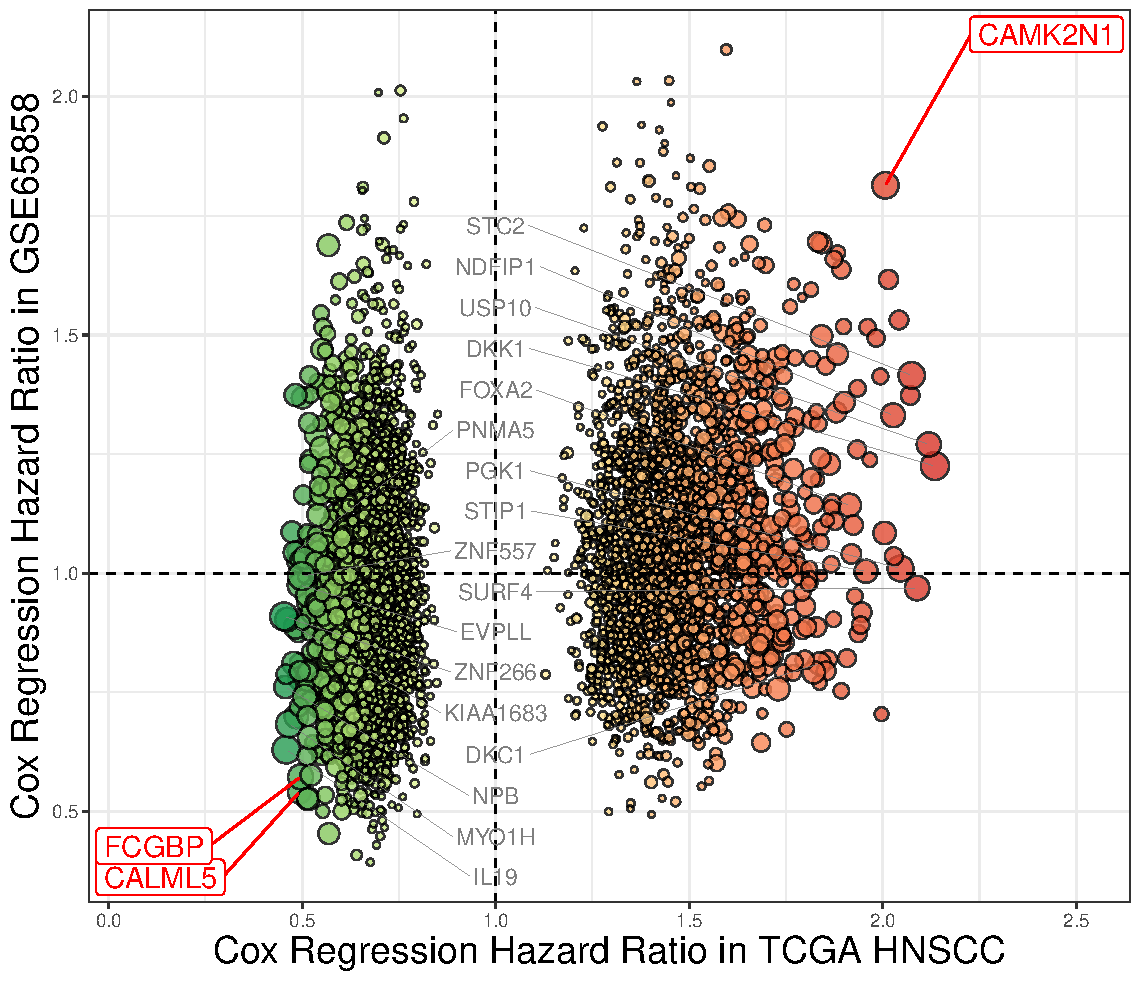
\includegraphics[width=7.5cm]{RplotH2H_TCGA_GSE65858_CoxHR.pdf}
    \caption{Cox's \hl{hazard ratios} from the two datasets (poor Pearson's correlation coefficient{\tiny ~\autocite{Schober2018}}, r = 0.27).}
    \end{subfigure}
%\hfill
    \begin{subfigure}[t]{0.15\textwidth}
    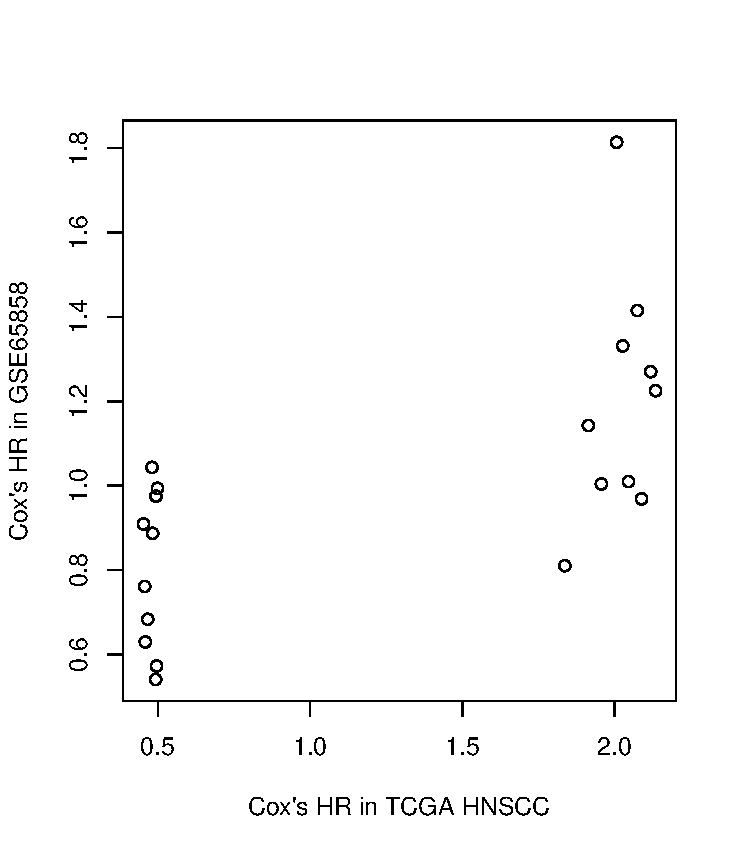
\includegraphics[width=2.5cm]{Rplot20_correlation_TCGA_GSE65858_CoxHR.pdf}
    \caption{Correlations of Cox's \hl{hazard ratios} of those 39 candidate genes (moderate Pearson's r = 0.68).}
    \end{subfigure}    
}   
{\captionsetup{labelformat=empty}    
\caption{A head-to-head comparison of Cox's hazard ratios (\hl{effect size}) from the two datasets. % (moderate correlation, Pearson's r = 0.68).
%(Pearson's r = 0.68).
%TCGA HNSCC and GSE65858 cohorts were applied for identification and validation of the candidate biomarkers in HNSCC.
%    (\textbf{a}) A total of 5404 genes had Cox's hazard ratios from TCGA HNSCC and GSE65858
%(Pearson's correlation, r = 0.27).
    %\acrshort{fdr}-\protect\textit{p}~values of less than 0.05 in TCGA HNSCC.
%    \textcolor{red}{CAMK2N1}, \textcolor{red}{CALML5}, \textcolor{red}{FCGBP}, and 17 other genes (marked in \textcolor{black}{black}) had hazard ratios (HRs) >$1.8$ or <$0.6$.
%    \textcolor{red}{Red spots}: $HR$s > 1.0 in TCGA HNSCC.
%    \textcolor{green}{Green spots}: $HR$s < 1.0 in TCGA HNSCC.
%    Sizes of spots: bigger for Kaplan--Meier \protect\textit{p}~values in TCGA HNSCC. %Please ensure intended meaning is retained.
%    (\textbf{b}) The 20 genes were extracted and shown. The hazard ratios of those genes have a moderate correlation between the two cohorts
%(Pearson's r = 0.68).
%    (X-axis: Hazard ratios of Cox proportional hazard regression model from TCGA HNSCC;
%    y-axis: Those values from GSE65858; TCGA: \acrlong{tcga}; HNSCC: \acrlong{hnscc}.)
    }}
%%%\label{fig:hazards_head2head_TCGA_GSE65858}
\end{figure}

\clearpage

%\subsection{Future Directions in Translational Medicine}


%\subsubsection*{Proteomics Validation}


%\subsubsection*{Laboratory Validation}


%\subsubsection*{Cancer Type-Agnostic Study}


\section{Summary of Modern HNSCC Therapy}

\thispagestyle{headings}
\markright{Discussion \hfill Poor survival rate of HNSCC patients \hfill}

\begin{minipage}[c]{0.40\linewidth}
\begin{outline}
\0
\0 Despite the improvements in surgery and systemic therapy,
%        \2 the survival of \acrshort{hnscc} has not improved; %worldwide~\autocite{hpa2019};
        \1 the five-year survival rate is under \hl{60\%} in TCGA;
        \1 the five-year survival rate* in Taiwan: \hl{55.13\% $\longrightarrow$ 56.03\%}  (2008-2018).
\0 To find more \hl{unknown pieces of a puzzle} $\longrightarrow$ survival.
\end{outline}

    {\tiny *\url{https://cris.hpa.gov.tw/pagepub/Home.aspx}}
\end{minipage}%\hspace{2mm}
%\begin{wrapfigure}{r}{0.3\textwidth}
\begin{minipage}[c]{0.55\linewidth}
    \raggedright
    \hfill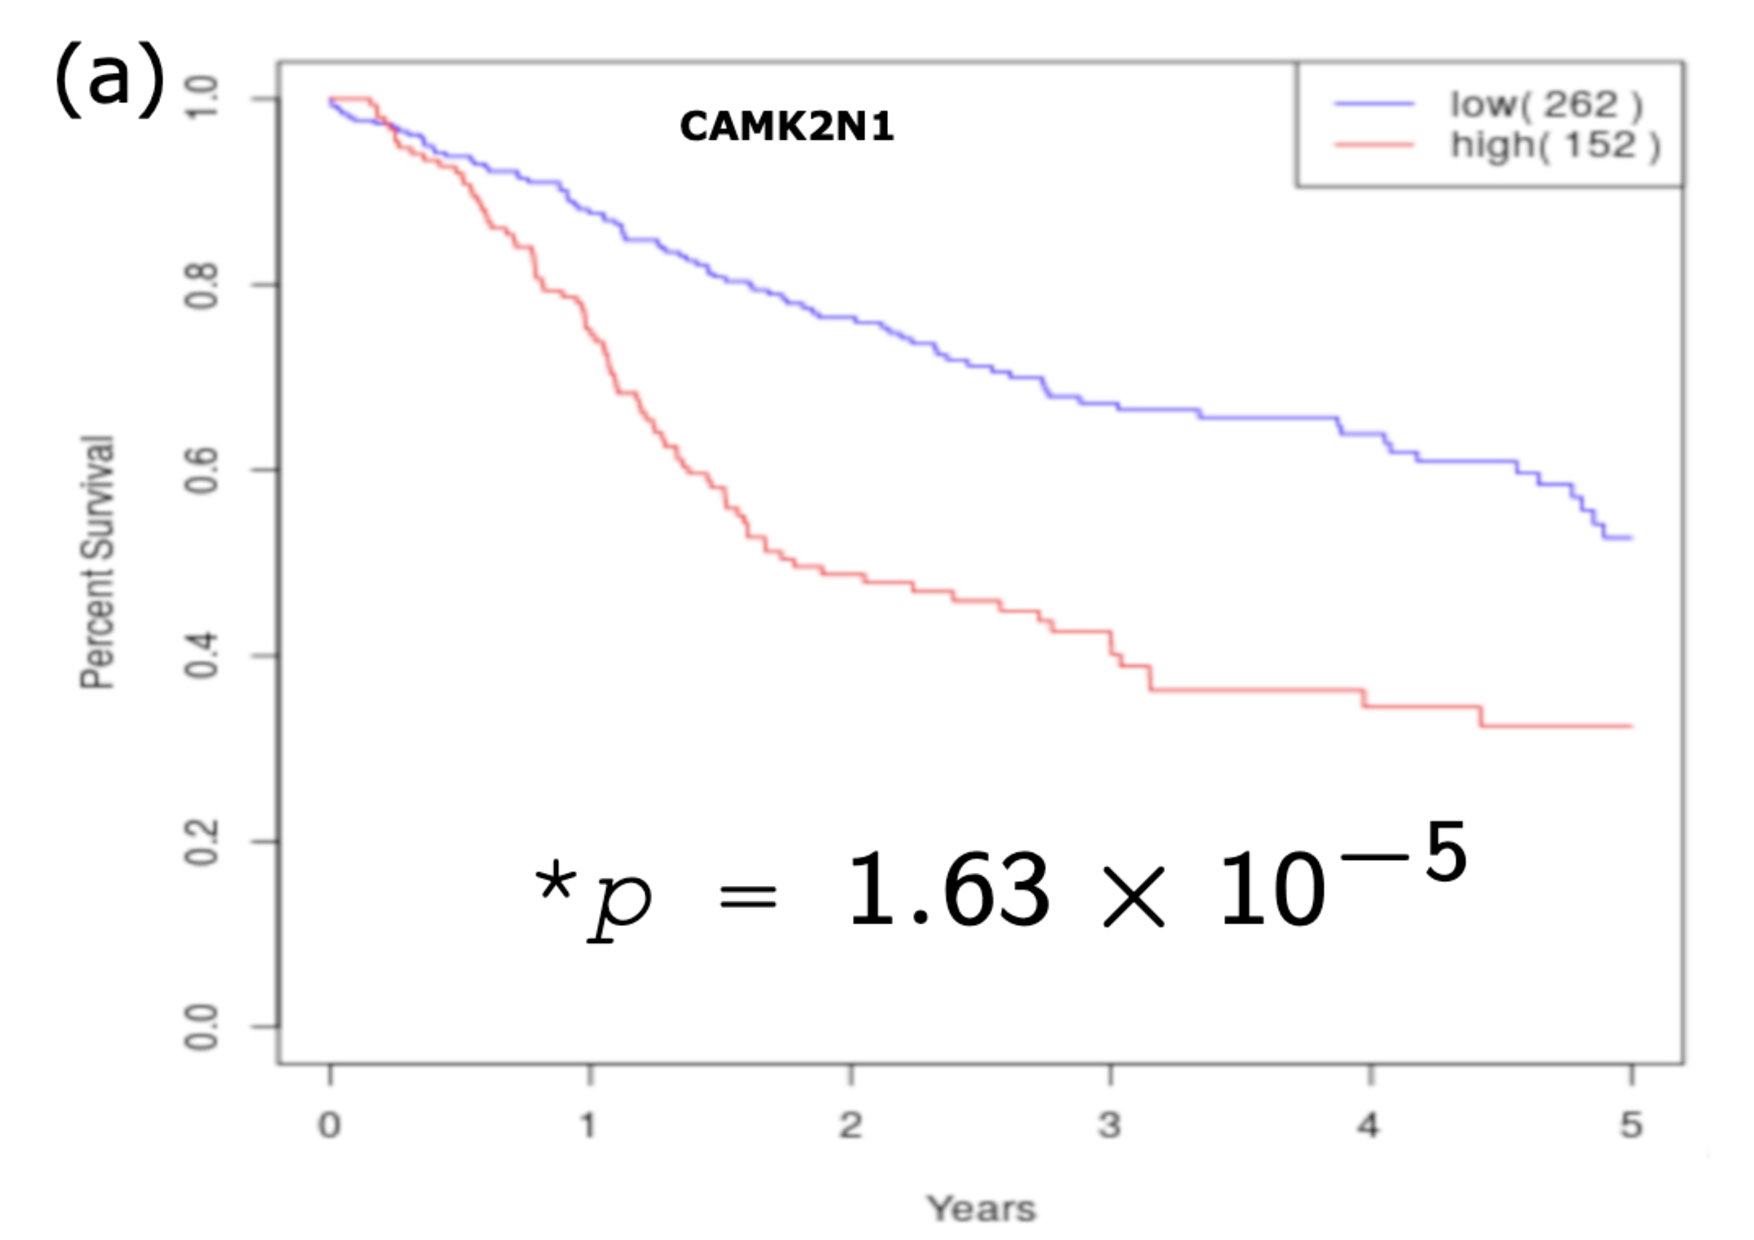
\includegraphics[width=7cm]{KMplot_CAMK2N1.pdf}
\end{minipage}




\clearpage



\section{Holistic Cancer Care} 

\thispagestyle{headings}
\markright{Discussion \hfill Holistic cancer care \hfill}

Holistic (whole) care: to care \hl{spirit}, \hl{emotion}, \hl{the body} of a person, and his \hl{social} relation.

It is the unknown piece of the puzzle in cancer care.\\
%Deep learning and holistic cancer care in the future: Chi2022
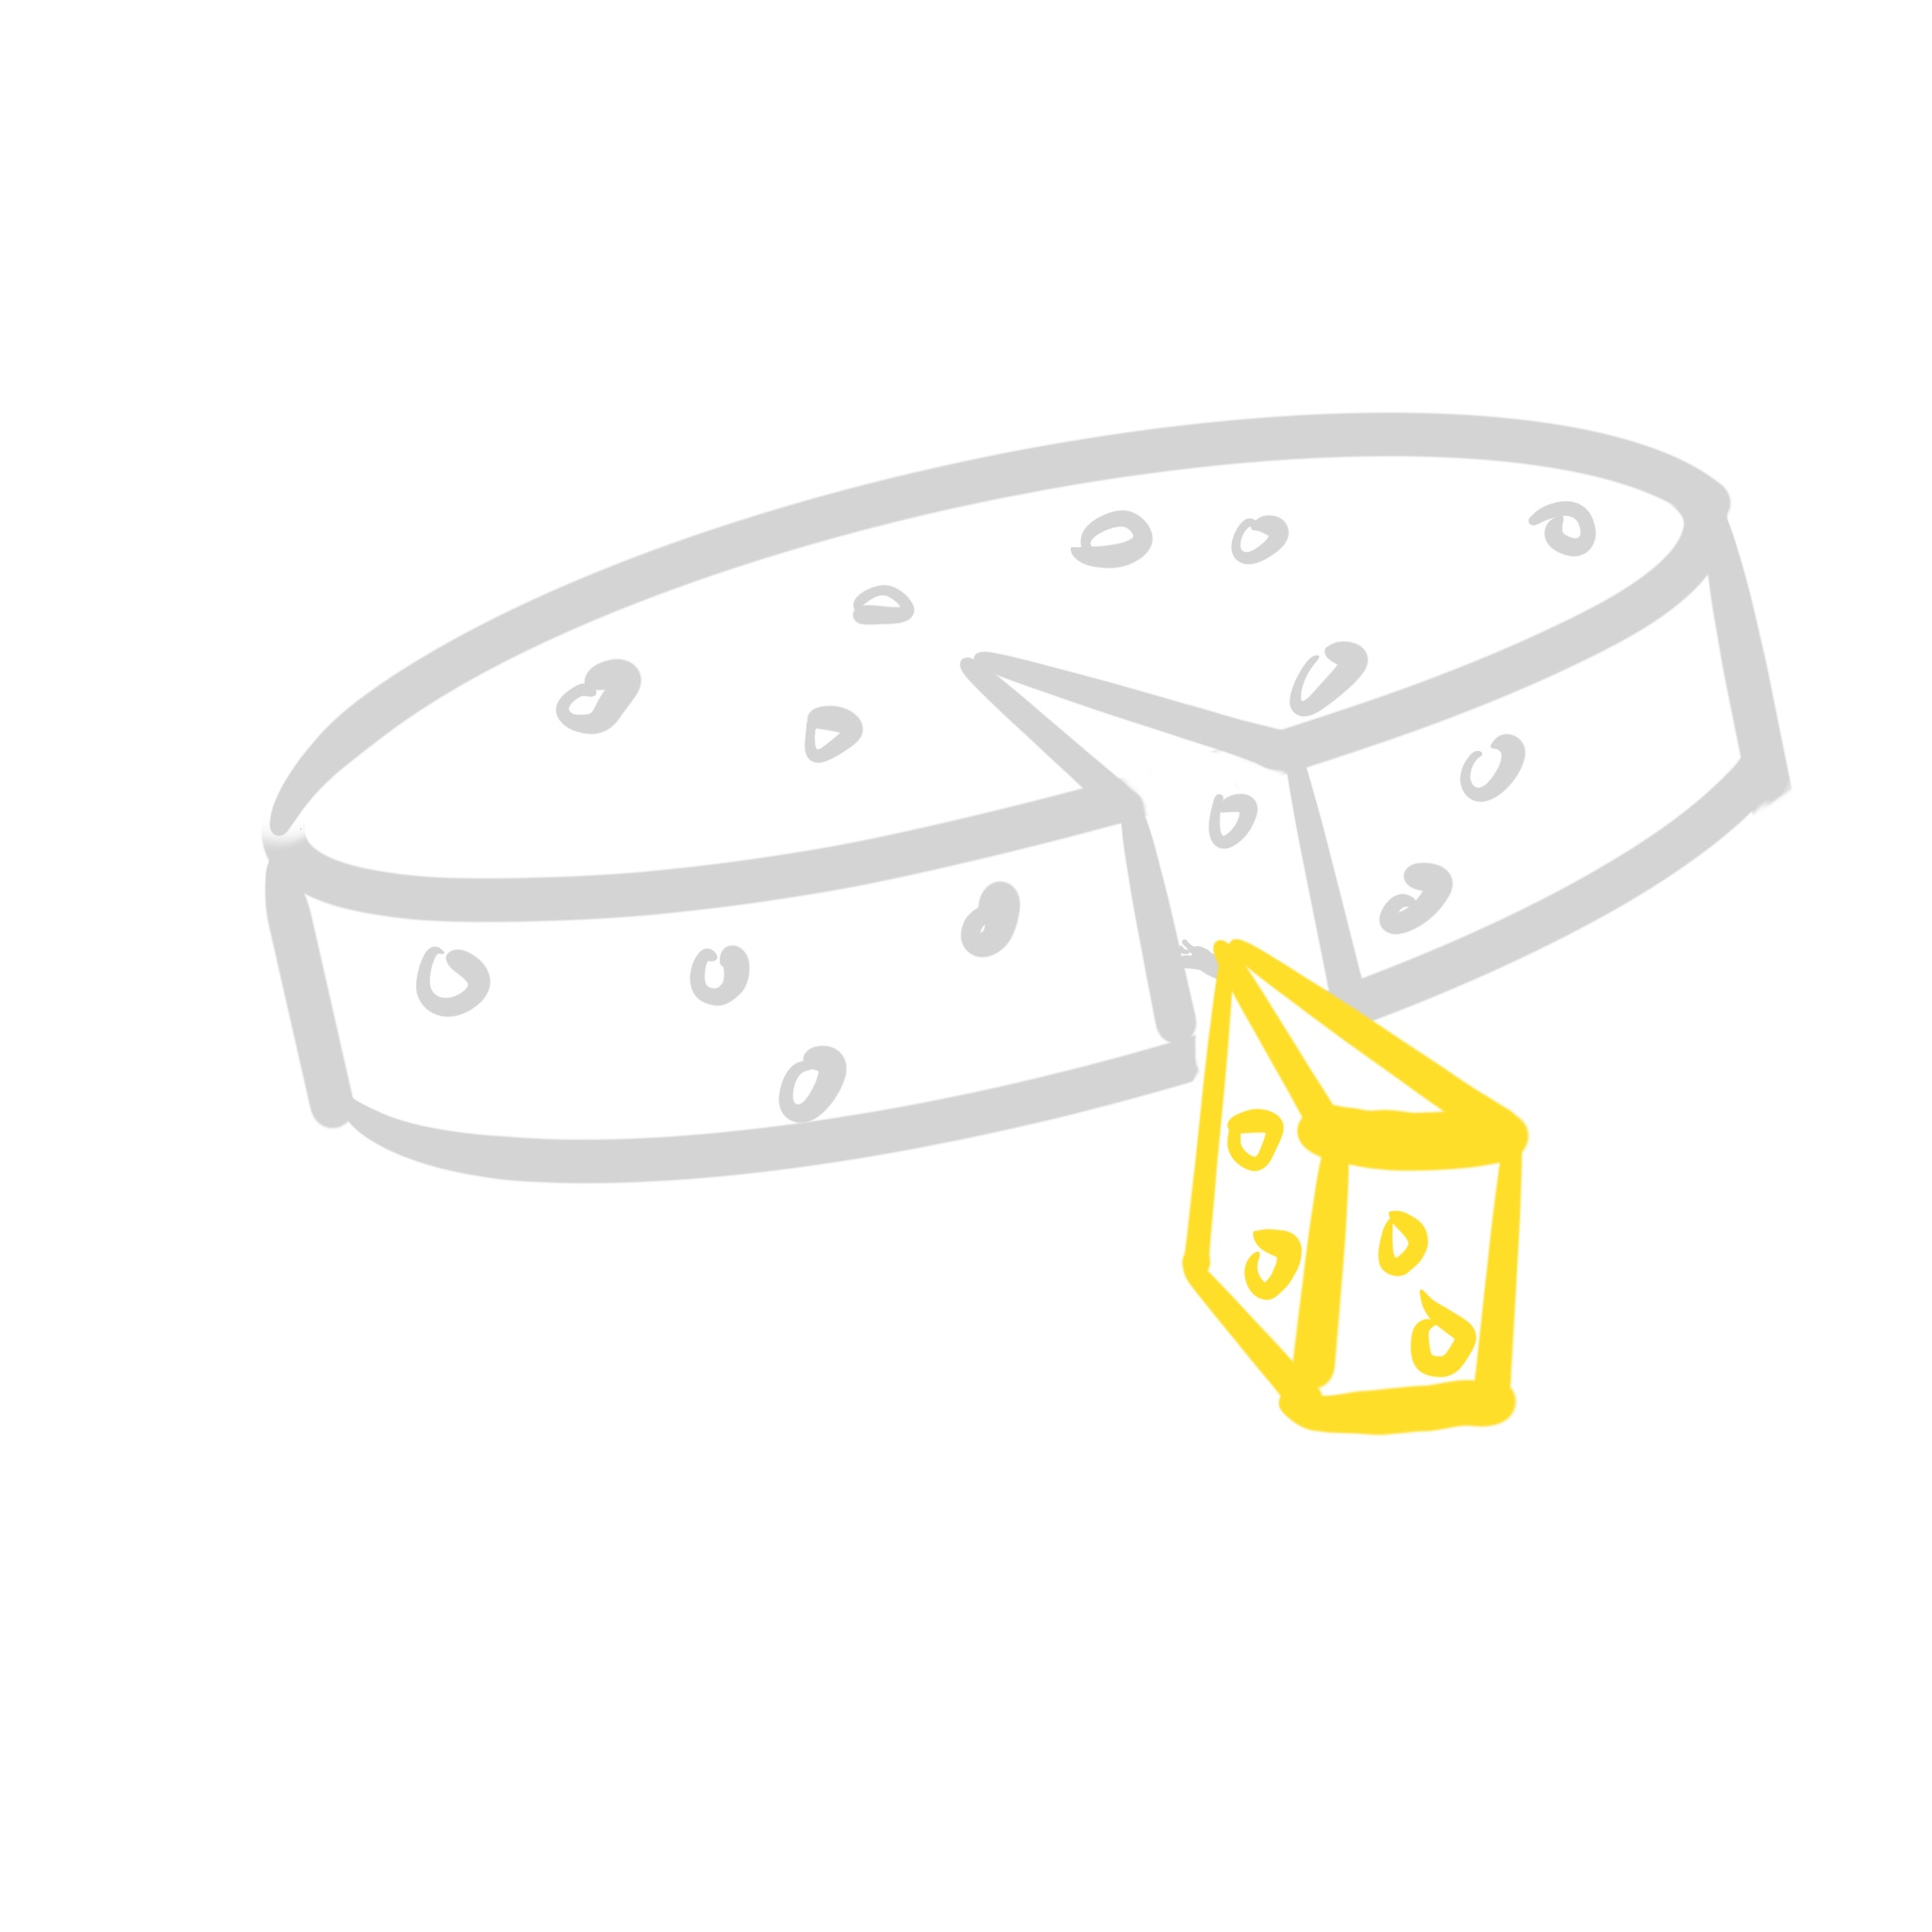
\includegraphics[width=4cm]{piece.jpg}
%%%%%%%%%%%%%%%%%%%%
%%%%%% carcinogenesis

\comm{ % comment it out

\begin{figure}[ht]

\begin{minipage}[c]{0.50\linewidth}
%\floatbox[{\capbeside\thisfloatsetup{capbesideposition={right,center},capbesidewidth=.25\linewidth,capbesidesep=quad}}]{figure}[\FBwidth]
%\centering

\setlength{\unitlength}{.78cm}
\begin{picture}(20, 10)(0,0) %(1,0.55038404)%
%\centering
  \put(0,0){\includegraphics[width=9.0cm]{Figure_5_holisticCare.pdf}}%
  \put(0.4, 9.3){\fontfamily{qcr}\selectfont
  \textbf{[Physician]}}%
  \put(6.0, 7.8){\fontfamily{qcr}\selectfont
  HNSCC}
\end{picture}
%\includegraphics[width=10cm]{Figure_5_holisticCare.pdf}
\end{minipage}
\hfill
\begin{minipage}[c]{0.40\linewidth}
%{\caption{
%The concept of holistic care for \acrshort{hnscc} patients. %MDPI: please confirm if the extra lines and frame need to be deleted.

Beyond carcinogenesis:\\
\hl{The mind--brain--body axis}~\autocite{Hsiao2012}
\small
\begin{outline}
\1 stress %ful environment(giant \textcolor{black}{black} arrow) 
will trigger an emotional response in mind
\1 brain releases stress hormones and inflammation signals in cells% in response to negative emotions.
\1 %The  body's internal environment (cells) 
altering epigenetic control in gene regulation and mRNA/miRNA expression %of cells
%Over a long time, the tissue/cells will be transformed into dysplasia and then 
\1 carcinogenesis~\autocite{Lutgendorf2010,Powell2013,Iftikhar2021} with help from known carcinogens
\end{outline}

\end{minipage}

%%%\label{fig:figure5}
\end{figure}
\clearpage

} % end of \comm
%%%%%%%%%%%%% care

\begin{figure}[ht]

\begin{minipage}[c]{0.50\linewidth}
%\floatbox[{\capbeside\thisfloatsetup{capbesideposition={right,center},capbesidewidth=.25\linewidth,capbesidesep=quad}}]{figure}[\FBwidth]
%\centering

\setlength{\unitlength}{.78cm}
\begin{picture}(20, 10)(0,0) %(1,0.55038404)%
%\centering
  \put(0,0){\includegraphics[width=9.0cm]{Figure_5_holisticCare.pdf}}%
  \put(0.4, 9.3){\fontfamily{qcr}\selectfont
  \textbf{[Physician]}}%
  \put(4.0, 9.3){\fontfamily{qcr}\selectfont
  \textbf{[Patient]}}%
  \put(6.0, 7.8){\fontfamily{qcr}\selectfont
  HNSCC}
\end{picture}
%\includegraphics[width=10cm]{Figure_5_holisticCare.pdf}
\end{minipage}
\hfill
\begin{minipage}[c]{0.45\linewidth}
%Holistic cancer care~\autocite{Mehta2019,Iftikhar2021}:

\small
\begin{outline}
\1 to give the \textcolor{green}{physical care}: surgery and/or systemic therapy (drug)
%\1 to support cancer patients' spiritual, emotional, physical, and socioeconomic needs

\1 \textcolor{green}{therapeutic relationship (TR)}~\autocite{Rogers1979}
    \2 the physicians' spiritual properties \hl{(empathy, sympathy, and compassion)} $\longrightarrow$ cancer patients
    \2 $\longrightarrow$ their \hl{self-compassion} $\longrightarrow$ \hl{resilience} $\longrightarrow$ their mind--brain--body axis $\longrightarrow$ the disease~\autocite{Hsiao2012}
\1 to reduce pain, to promote \hl{survival} from cancer

\end{outline}

\end{minipage}

%%%\label{fig:figure5}
\end{figure}
\clearpage




\section*{Conclusions} % 5
\thispagestyle{headings}
\markright{Conclusions \hfill Physical care \hfill}

\begin{outline}

\1 The microenvironment of HNSCC, influenced by the mind--brain--body axis~\autocite{Hsiao2012}
    \2 Four \hl{biomarker} candidates---TMSB4X, CAMK2N1, CALML5, and FCGBP---which are all heavily associated with the prognosis of \acrlong{os}~\autocite{Chi2017, Chi2021};
    \2 TMSB4X might promote metastasis of \hl{neck lymph nodes} (N+);

%    \2 further exploration and understanding using \hl{holistic} multi-parametric approaches
%\1 Good using a placebo effect in HNSCC cancer care
%    \2 dorsolateral prefrontal cortex~\autocite{Carlino2011} is the origin of a placebo effect
%    \2 Confidence/trust (i.e., \hl{TR}) might promote healing through a mind--brain--body connection manner
    

\1 A grant proposal (machine learning algorithm---deep learning)
    \2 CAMK2N1 might involved in positive \textcolor{red}{surgical margin};
%        \2 CAMK2N1 has moderate correlation with N+ (Pearson's r = 0.07) :-)
    \2 CAMK2N1 might predict \textcolor{red}{neck metastasis} in clinical N0 neck before surgery;
\1 A grant proposal for validation of CAMK2N1 by \hl{laboratory experiments}.

\end{outline}

%
\clearpage

\thispagestyle{headings}
\markright{Conclusions \hfill Spiritual care \hfill}

\begin{outline}


%\1 More holistic features in HNSCC dataset
\1 The HNSCC dataset must collect those "\hl{holistic features}" for further \hl{holistic biomarker} in personalized medicine, from
    \2 electric healthcare records (EHR);
    \2 A grant proposal: \hl{wearable device} (heart rate variability, HRV) is correlation with patient's emotional stress $\longrightarrow$ \hl{malignant transformation} of oral lesions (e.g., verrucous hyperplasia);
    %患者配戴 HRV 心率手錶,檢測治療期間,追蹤期間(一年),患者的心理壓力指數(HRV 數字越小表示交感神經越亢奮、壓力指數高)。
    \2 spiritual assessment (the meaning of life, hope, love/be loved, forgive/be forgiven, relationship with the Most High).
    %Thus, we suggest that electric healthcare records (EHR) should include physical, pathological, and psychological data, and even more spiritual information. The \acrshort{tcga} might collect those "holistic features"  (\textcolor{green}{green} dashed line) for further study of personalized medicine.
\1 A \hl{professional spiritual caregiver} 
    \2 \hl{Mindfulness meditation} is helpful to cancer patients
%    \2 confess for not taking care of their bodies and spirits in the past (\hl{causality})
%    \2 give sincere thanks for their physical body's hard work
\end{outline}
\begin{figure}
    \centering
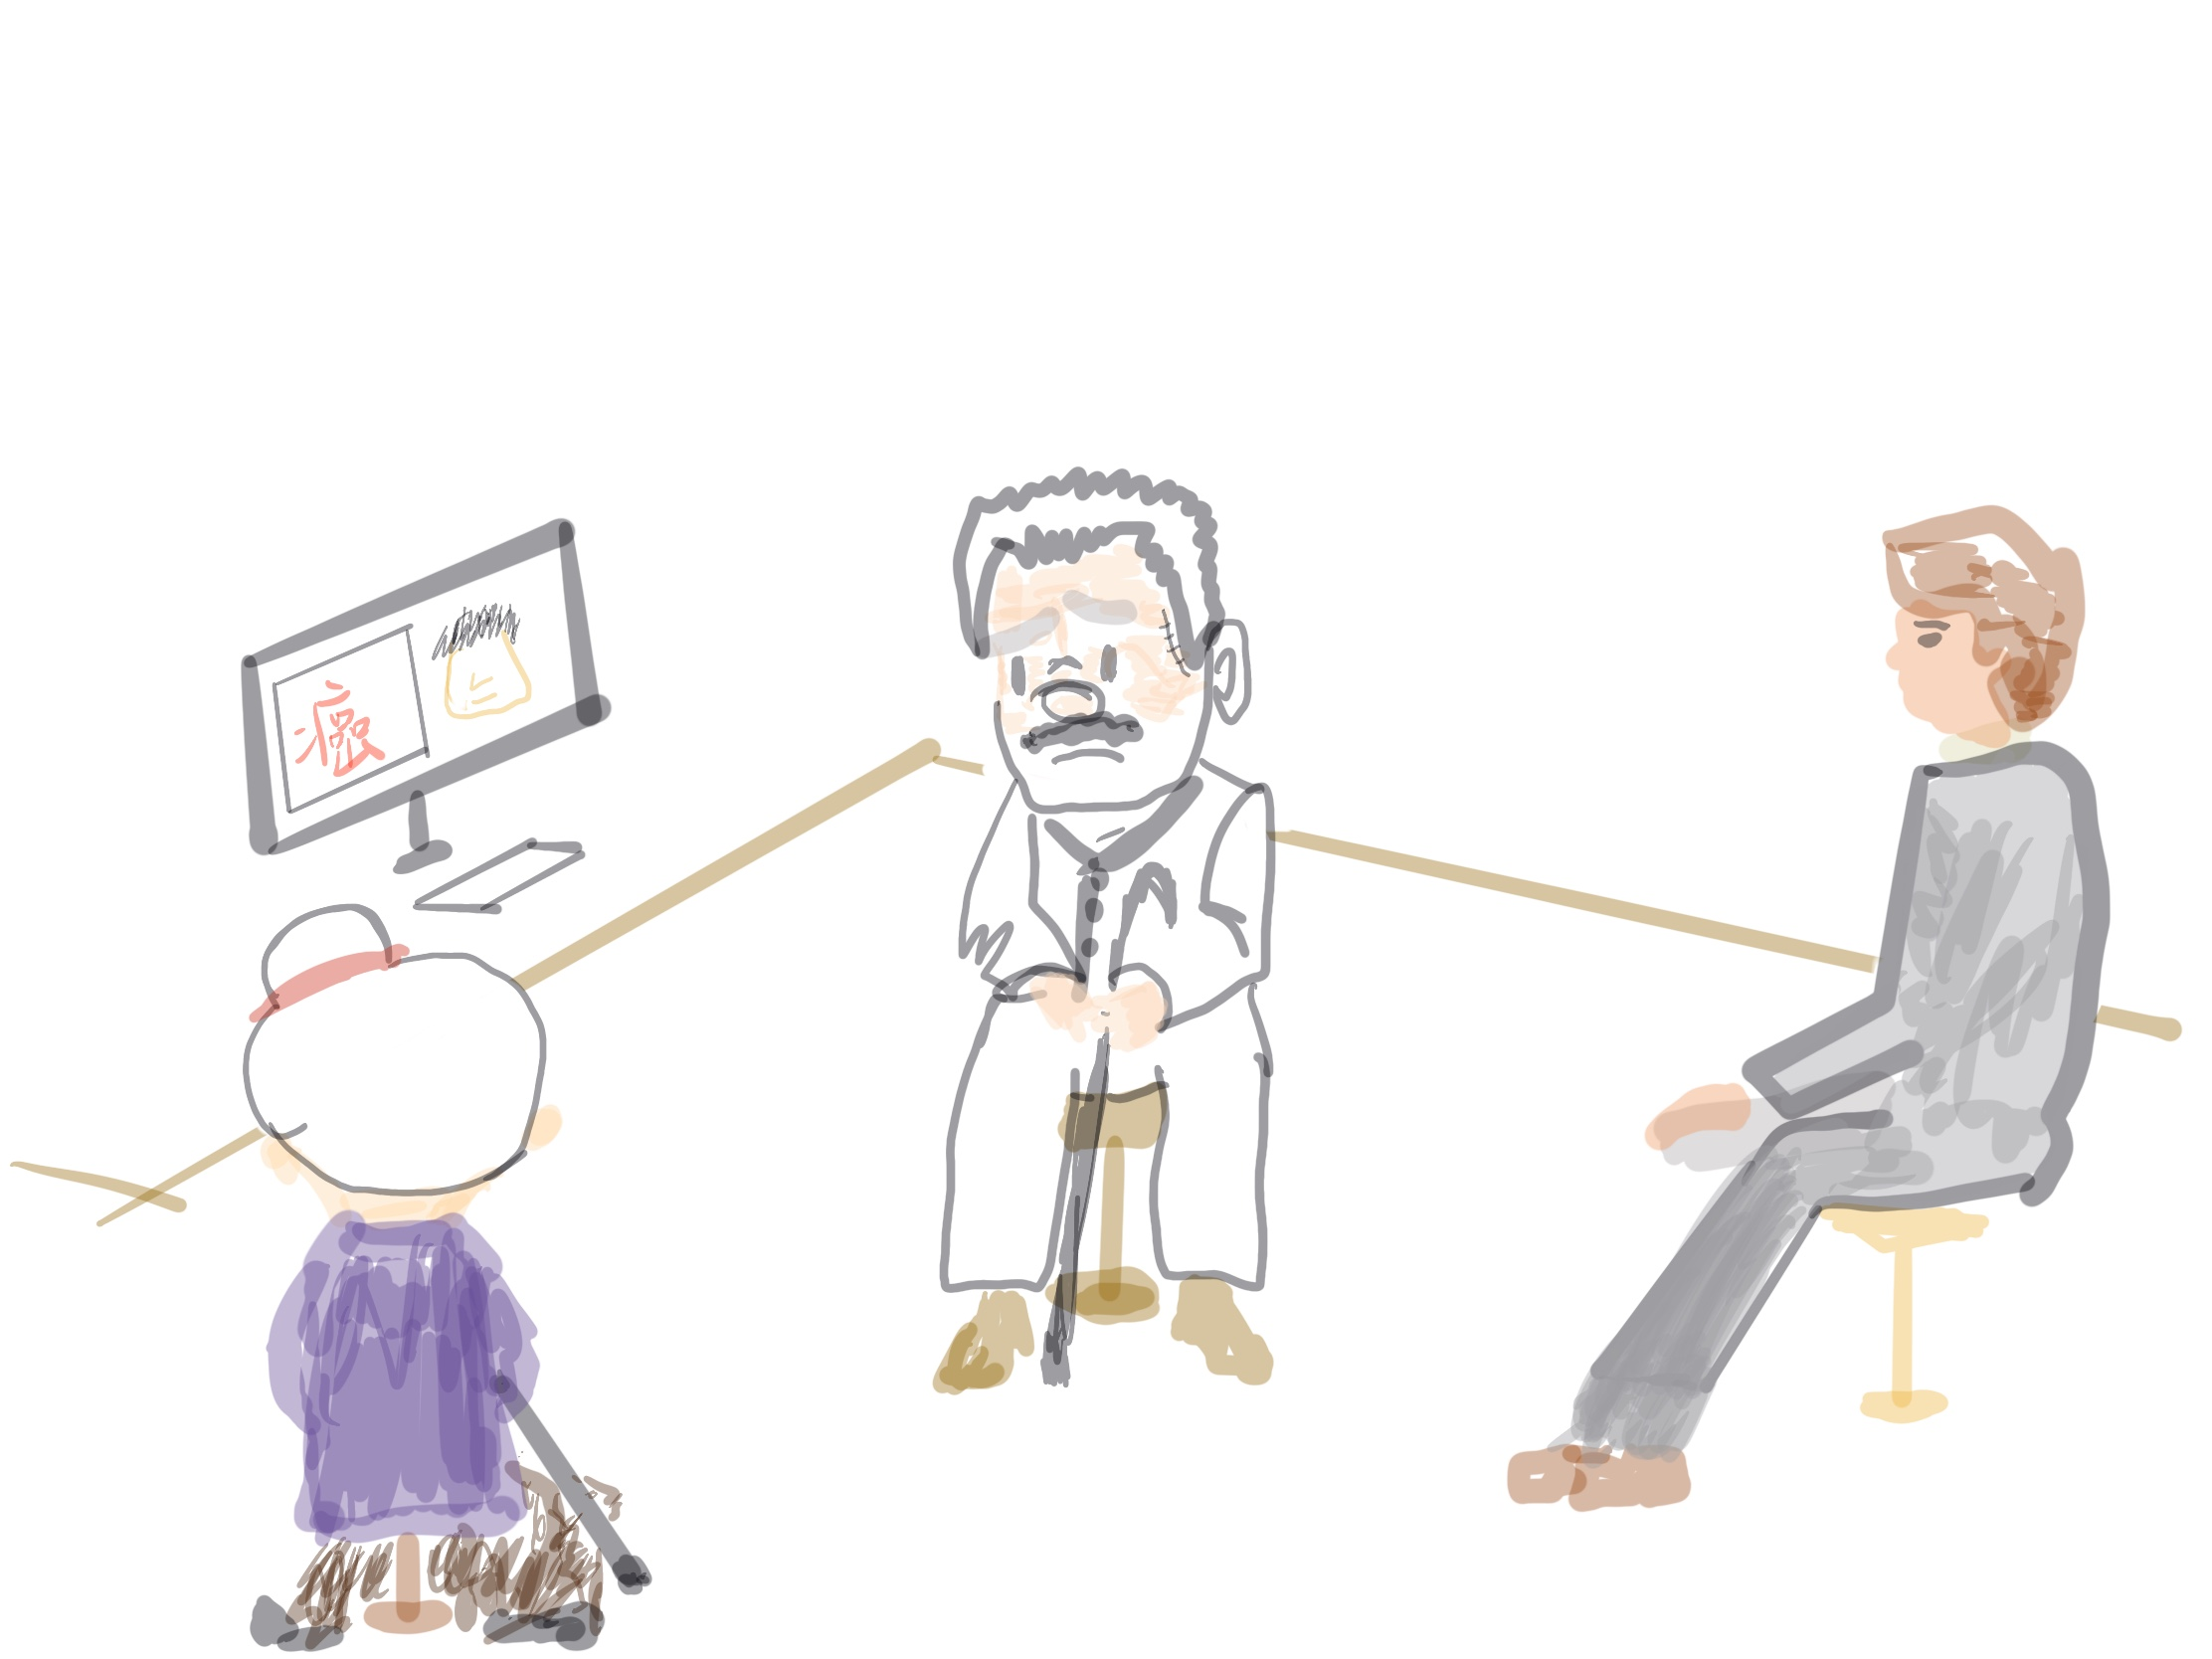
\includegraphics[width=11cm]{family_meeting_Cheung202109.jpg}
\end{figure}

%人俯仰於天地之間
%順從四季氣候變化
%保養正氣陶冶性情
%自我療癒身心靈疾病
%自他不二 心存正念 向內看,解決苦之源
%1.衷心懺悔
%2.真心感謝
%3.誠意祝福
%4.永存善念 慈悲
%5.心無恐懼: 情志養生
%每位醫師都可以成為「創傷知情者」幫助我們身邊的病患,懂他的心靈創傷,讓他有安全感, 才有機會改變疾病的走向
%"每一位患者都有自癒能力, 我們知情之後, 也要逐步讓他本人知情, 看見之後, 在良好的「治療關係」中, 協助他們漸漸找回自己的療癒。(以他們自己的腳步)"
%解說:患者的自癒力就是復原力(resilience),  強調「治療關係」(安全、 信任、 分享權力、 自決) 以及”知情”(暸解過往創傷經驗對自身的影響,進而開始療癒的過程)的重要性。
%%%%%%%%%%%%%%%%%%%%%%%%%%%%%%%%%%%%%%%%%%%%%%%%%%%%%%%%%%%%%%%
%\clearpage
%\thispagestyle{headings}
%\markright{Conclusions \hfill An example of holistic assessment in dental record \hfill}

%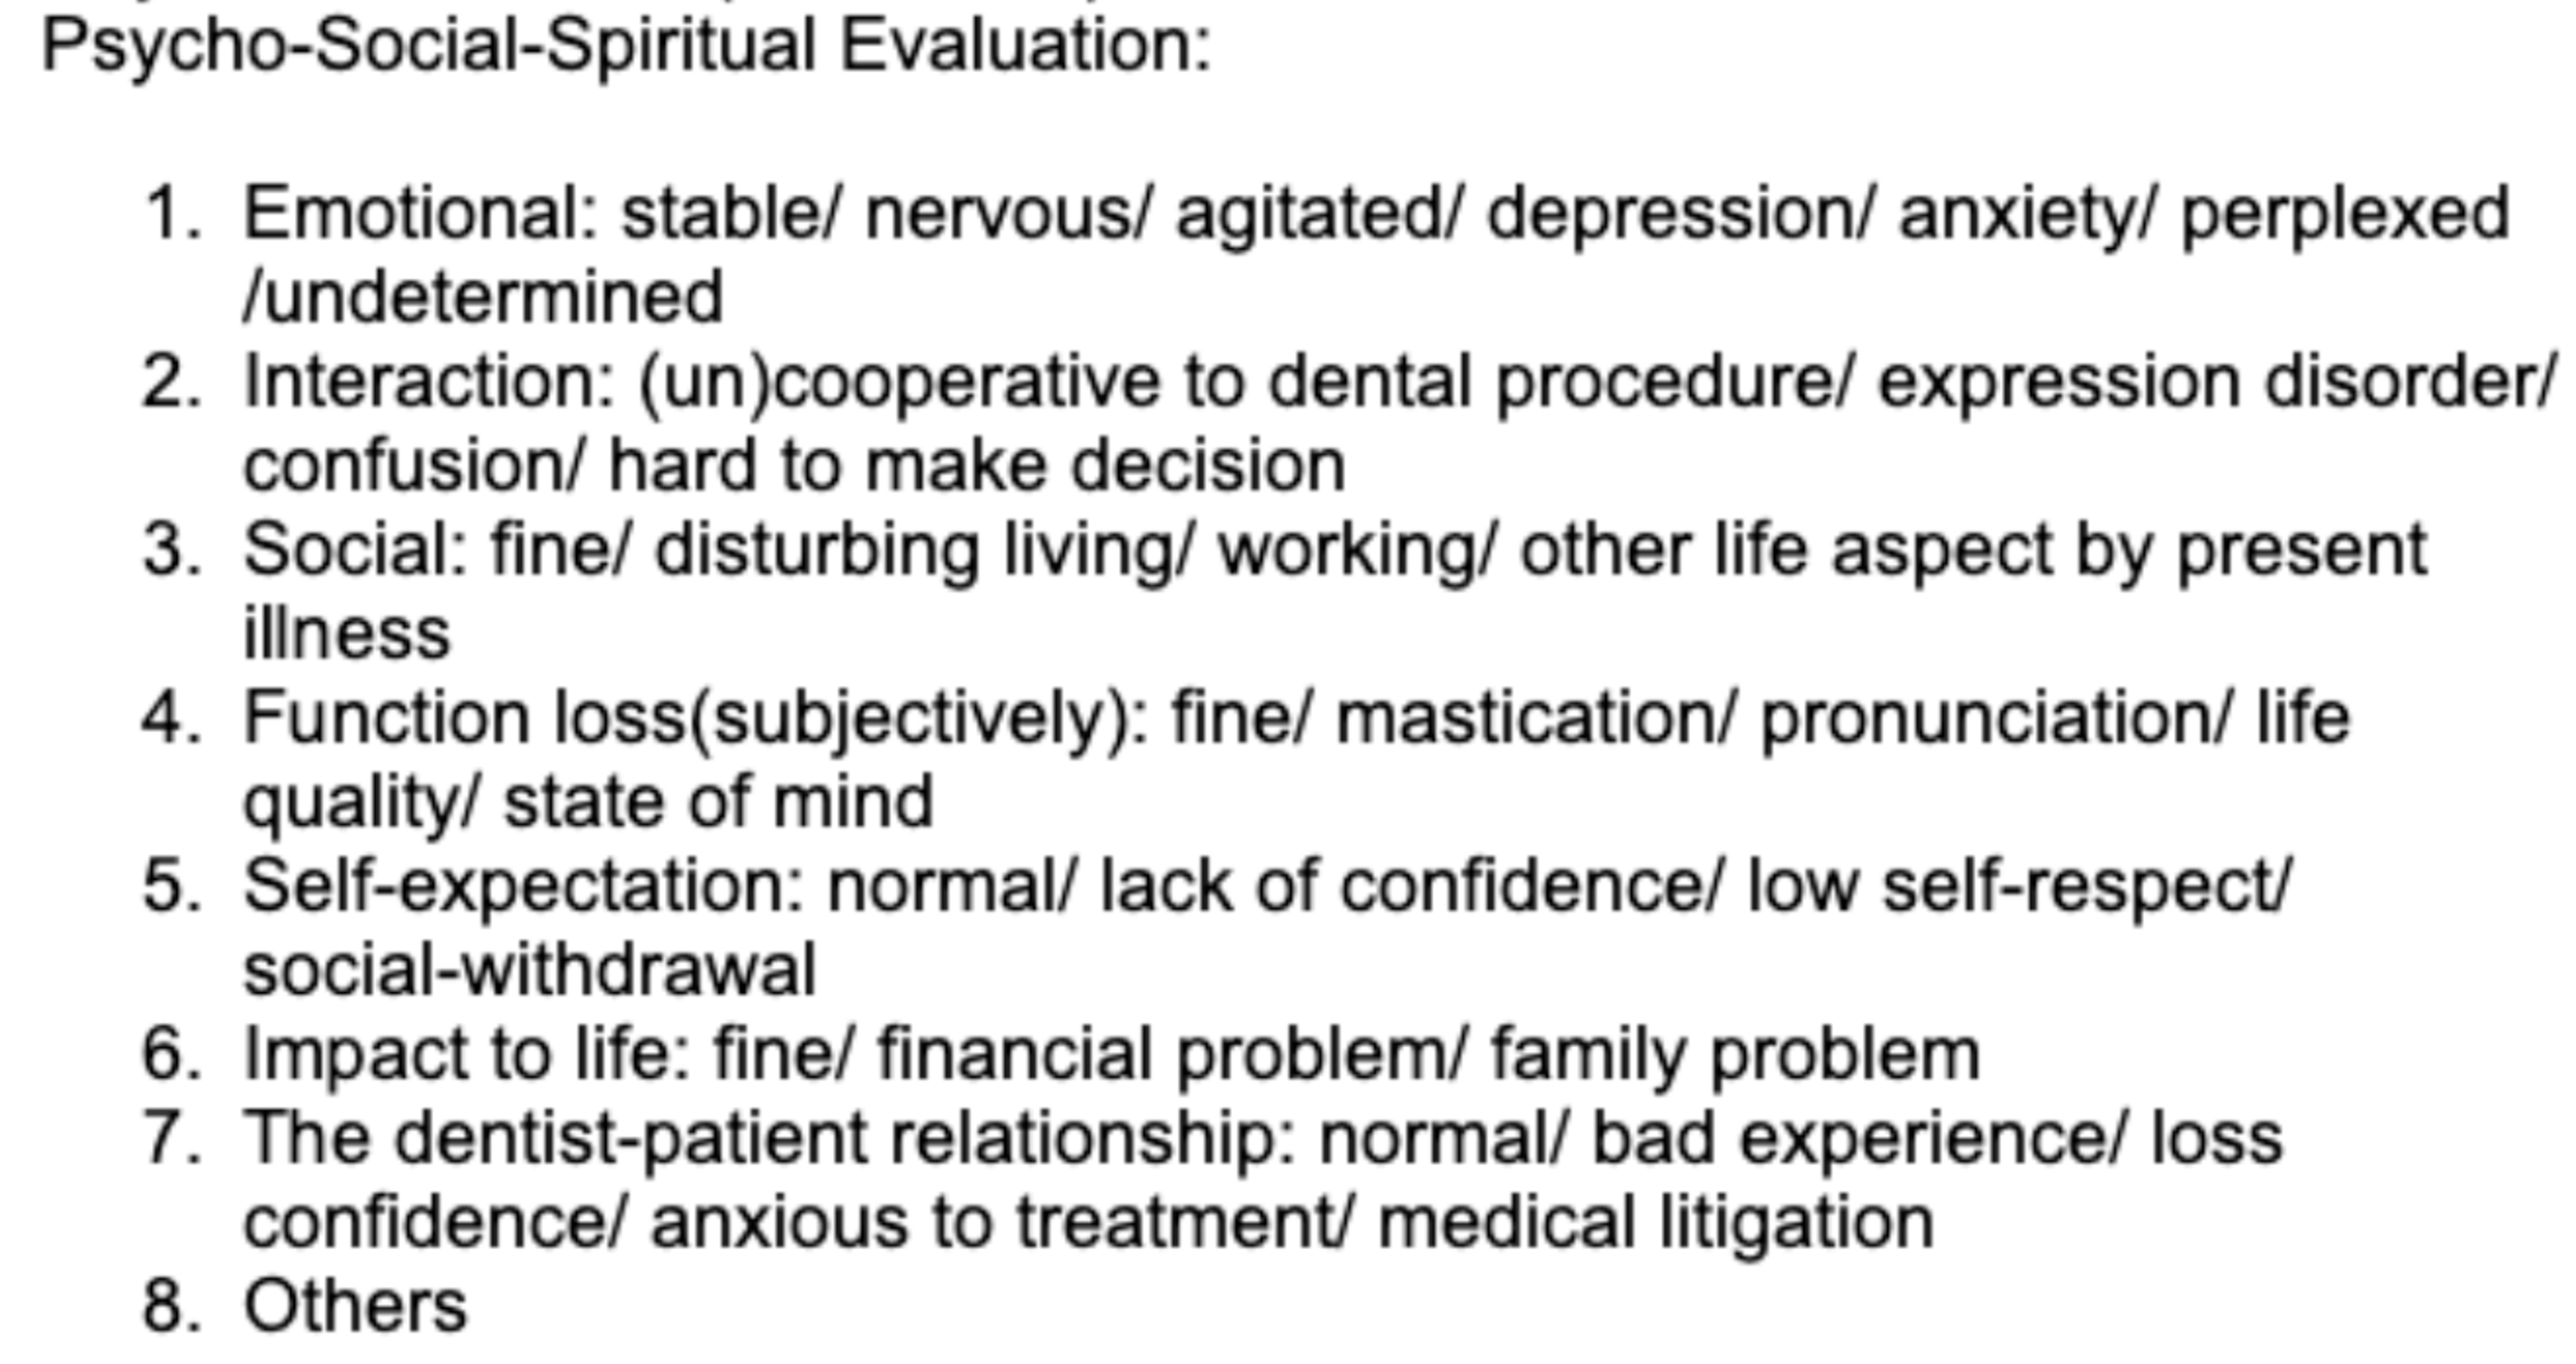
\includegraphics[height=6.5cm, width=6.5cm]{Holistic_EHR_TMUH_English.pdf}\hfill
%\includegraphics[height=4.5cm,width=7.5cm]{Holistic_EHR_TMUH_Chinese.pdf}


%\clearpage

%%%%
%\section*{Take Home Message}
%\thispagestyle{headings}
%\markright{Take home message \hfill  \hfill}
%\includegraphics[width=14.5cm]{PCA_CarlRogers.pdf}

\clearpage
%%%%%%%






% references
\thispagestyle{headings} % No slide header and footer

%\bibliographystyle{unsrt}
%\bibliography{TCGA_margin_cutoff.bib, betel.bib, TMSB4X.bib, pvalueTex.bib}
\printbibliography % for biblatex
\clearpage

%------------------------------------------------

\thispagestyle{empty} % No slide header and footer

\begin{tikzpicture}[remember picture,overlay] % Background box
  \node [xshift=\paperwidth/2,yshift=\paperheight/2] at (current page.south west)
    [rectangle,fill,inner sep=0pt,minimum width=\paperwidth,minimum height=\paperheight/2.1,top color=myblue,bottom color=myblue]{}; % Change the height of the box, its colors and position on the page here
\end{tikzpicture}
% Text within the box
\begin{flushright}
  \vspace{1.6cm}
  \color{white}\sffamily
  {\bfseries\Large Thanks Professors \\Comments and Suggestions\par}% Title
  \vspace{0.5cm}
  \normalsize
%  \myauthor\par % Author name
%  \mydate\par % Date
  \myuni\par
  \vfill
\end{flushright}
%李友專
%蕭宏昇
%吳駿翃
%王美娟
%楊欣洲
%王皓青
%張資昊
%----------------------------------------------------------------------------------------
%
\end{document}


%%%%
報告親愛的老師,晚安

1)謝謝老師,百忙之中能參加祁力行的口試 (日期時間:2022/01/12 11:00-12:00, Wednesday);
2)地點(***已變更,不在吳興街),改為「台北市大安區基隆路二段172-1號15樓討論室A」(這是北醫大安校區)。
3)敬請老師填寫「校園訪客登記:數位訪客證」存在手機中即可,
https://glbsys.tmu.edu.tw/guestsign/Apply.aspx
洽公單位請填寫:醫學資訊研究所

4)力行的論文是以口腔癌的治療為骨幹,嵌入 Chi2017 及 Chi2021 兩篇文章,融合改寫、加上deep learning與全人口腔癌照護的概念,總集而成。
博士論文初稿:https://drive.google.com/file/d/1C5iNhcdUzL1LnRiHZ5ZF8LAhZaPMamMB/view?usp=drivesdk

以下為簡介:
Chi2017> 由口腔癌病理檢體,MS mass spectrometry 打碎飛出來的蛋白質片段,來找出生物標記 biomarker (看看什麼基因、蛋白質表現多的,和癌症病患的存活率有關)
發表的文章 https://www.nature.com/articles/s41598-017-09539-w

Chi2021> 則是由口腔癌病理檢體,NGS 基因定序,來找出生物標記 biomarker (看看什麼基因、蛋白質表現多的,和癌症病患的存活率有關)
發表的文章 https://www.mdpi.com/2075-4426/11/8/782/htm;另有video 簡介(十分鐘)
https://encyclopedia.pub/16116

以上報告 麻煩老師了
下週見,謝謝老師
力行敬上
% spared code

%------------------------------------------------

%pstricks

\begin{pspicture}(2008, 0)(2018,100)
\psset{unit=.75cm}
\psaxes[labelFontSize=\scriptstyle]{<->}%
%  (0,0)(2008,0)(2018,100)[$x$-axis,-90][$y$-axis,180]
  \psline[linewidth=1.5pt,
  linecolor=red](2009,55)(2017,57)
\end{pspicture}

\section*{x Verbatim}

How to include a theorem in this presentation:
\begin{verbatim}
\mybox{0.8\textwidth}{
\begin{theorem}[Murphy (1949)]
Anything that can go wrong, will go wrong.
\end{theorem}
}
\end{verbatim}

\clearpage

%------------------------------------------------



\subsection*{Figure}

%\clearfloatsetup{figure}
%\floatsetup[figure]{style=no,capposition=beside,capbesideposition={center,inside},capbesideframe=yes,facing=yes}

\begin{figure}[ht]
\floatbox[{\capbeside\thisfloatsetup{capbesideposition={right,center},capbesidewidth=.35\linewidth,capbesidesep=quad}}]{figure}[\FBwidth]
{\captionsetup{labelformat=empty} \caption{\texttt{capbesidesep=quad}. I want to thank Sonia. The caption can contain any text but needs to describe the image with enough detail for a reader to completely understand the image.}}
{\includegraphics[width=0.6\textwidth]{placeholder.jpg}}
\end{figure}
%\includegraphics[width=9cm]{placeholder}

%\sidecaptionvpos{c}
%\caption{I want to thank Sonia.}
%\end{captionbeside}


\clearpage

%------------------------------------------------

